\section{Introduction}

Magnetic resonance imaging (\gls*{MRI}) is a non-invasive imaging technique used to visualize the structure and function of the human body.
By employing strong magnetic fields and radiofrequency pulses to manipulate the magnetic moments of atomic nuclei within tissues, subsequent changes in bulk magnetization transverse to the main magnetic field can be detected and reconstructed into high-resolution images.

Myelin water imaging (\gls*{MWI}) is a specialized \gls*{MRI} technique designed to quantify myelin content in white matter tissue.
Myelin, a lipid-rich substance forming an insulating sheath around axons, facilitates rapid and efficient electrical impulse conduction;
its degradation, as seen in diseases such as multiple sclerosis, impairs neural function.
\gls*{MWI} exploits the differing transverse relaxation times ($T_2$) of water in distinct tissue compartments.
Specifically, the $T_2$ of water within the myelinated lipid bilayers is several times shorter than that of the surrounding tissue.
This gives rise to a transverse magnetization which is composed of signal components decaying at different relaxation rates, measured for example using a multi-spin echo (\gls*{MSE}) scan with uniform echo spacing.

Quantitative analysis of \gls*{MSE} signals commonly involves multi-exponential decomposition, where the observed signal is modelled as a sum of exponentially decaying components, each characterized by a distinct $T_2$ relaxation time~\citep{doucette_decaes_2020}.
The myelin water fraction (\gls*{MWF}), defined as the fraction of signal attributed to rapidly decaying $T_2$ components, is a marker for myelin content.
However, estimating $T_2$ distributions and their derived biomarkers from \gls*{MSE} data is challenging.
Traditional methods, such as nonnegative least squares (\gls*{NNLS}), yield point estimates that are sensitive to noise and require regularization for stability;
moreover, they provide no measure of uncertainty in the $T_2$ spectrum, leaving the reliability of derived metrics unassessed.
A more robust approach considers the entire space of plausible $T_2$ distributions.

Bayesian posterior sampling, which explores the full posterior distribution of $T_2$ spectra consistent with the measured signal, is well-suited for this task.
This approach not only provides estimates of the mean $T_2$ distribution but also enables the quantification of uncertainty for individual $T_2$ components and derived metrics, such as \gls*{MWF}.
However, sampling from the posterior distribution can be computationally demanding for high-dimensional problems.
To address this, we propose a hybrid framework that combines traditional posterior sampling with a learned change-of-variables obtained through variational inference.
We train a conditional normalizing flow to approximate the true posterior distribution and utilize the resulting learned bijection as a preconditioning transformation for traditional Bayesian sampling methods, such as Metropolis--Hastings or Langevin dynamics.
While this proposed framework contains a learned component, the network serves primarily as a change of variables that preconditions the problem geometry for more efficient sampling, analogous to preconditioners in iterative solvers for linear inverse problems and to coordinate transformations in numerical integration.
Additionally, we introduce a novel, interpretable, shallow prior over the space of $T_2$ distributions based on the Aitchison geometry, learned simultaneously with the approximate posterior.
We demonstrate that our integrated approach enables efficient posterior sampling, leading to improved estimation of $T_2$ distributions and \gls*{MWF} in myelin water imaging.

\Cref{fig:invivo_comparison} illustrates representative in vivo estimates.

\begin{figure}[htbp]
    \centering
    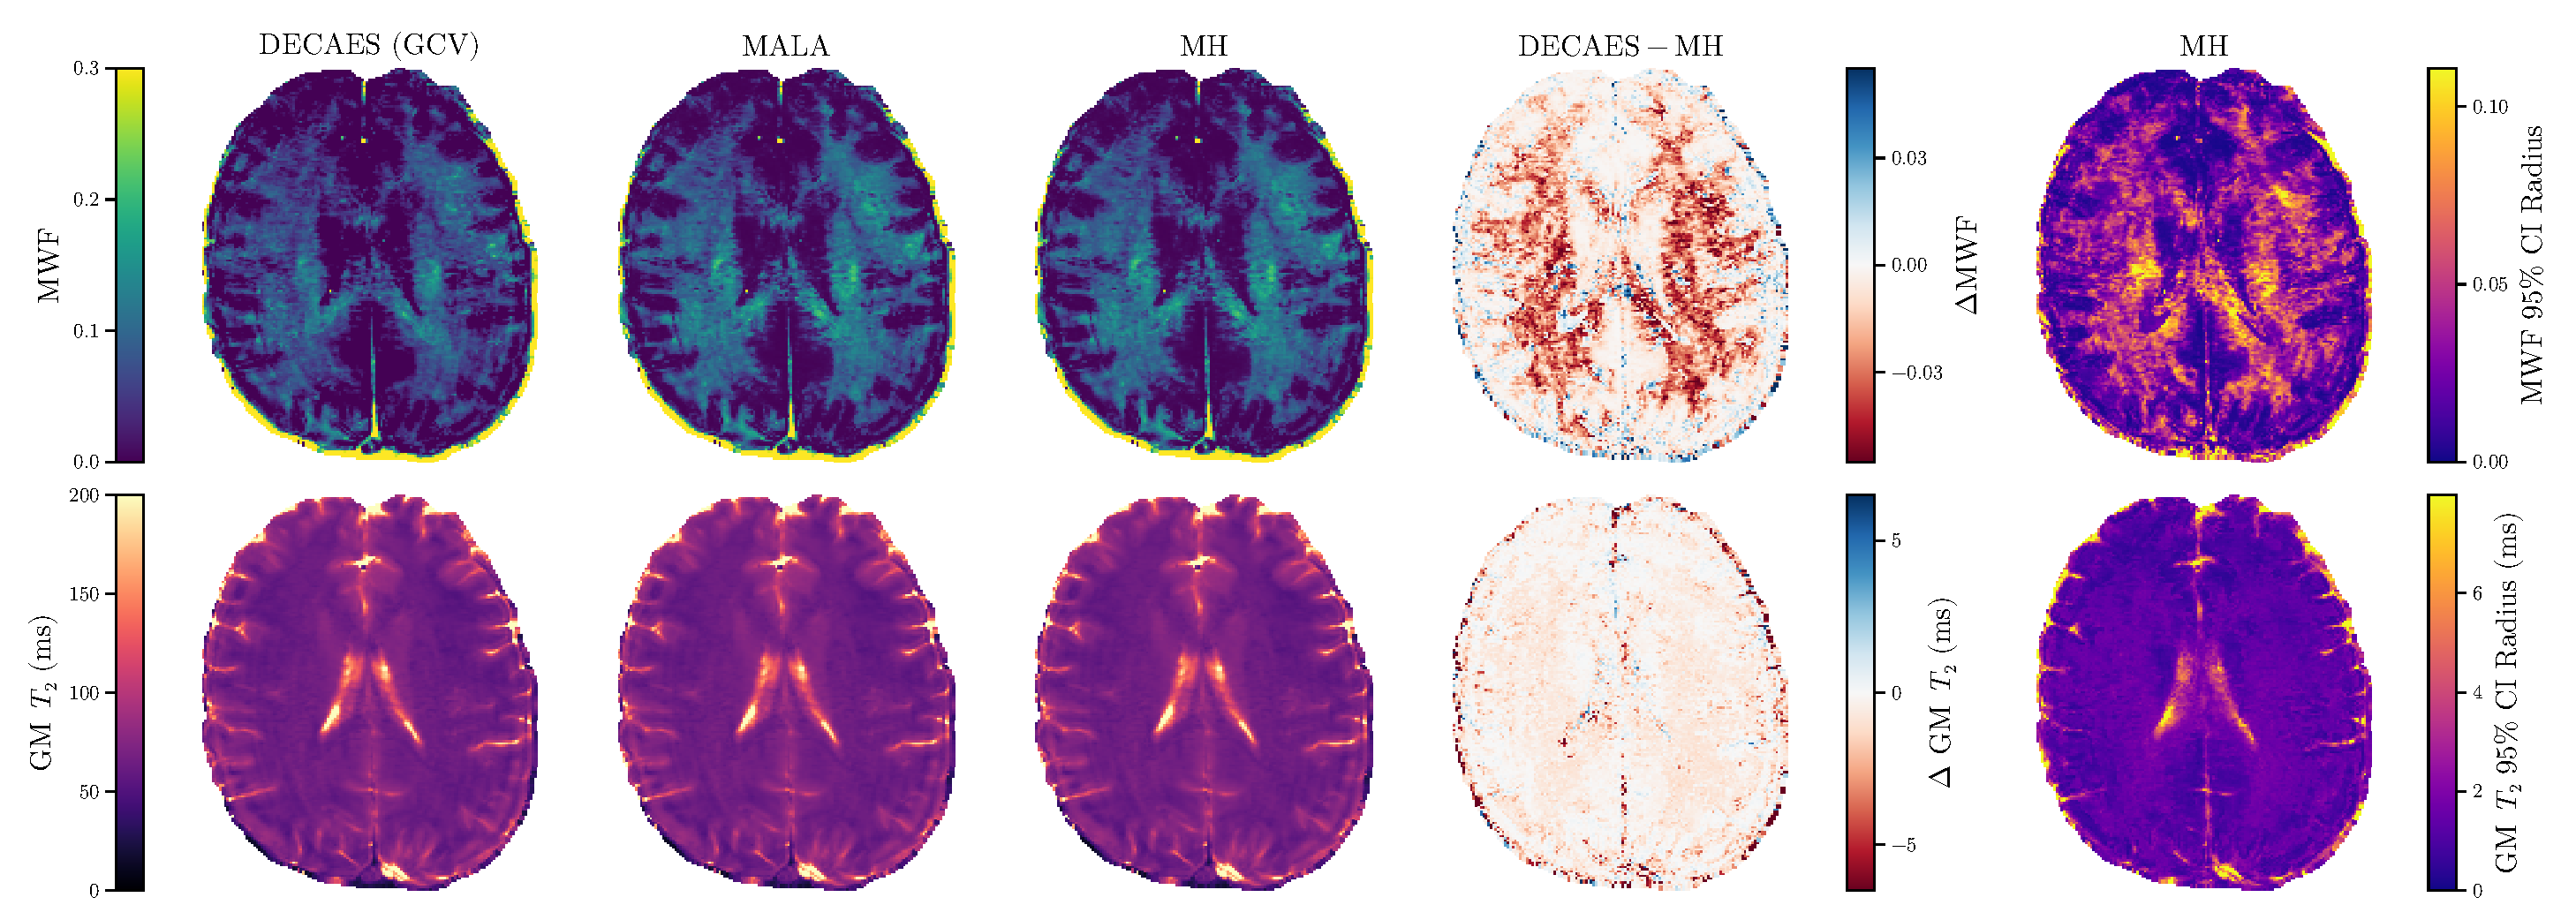
\includegraphics[width=\linewidth]{figures/compare_inference_method_slices.pdf}
    \caption{Representative in vivo brain biomarker maps for a single axial slice.
        Rows show \gls*{MWF} and geometric mean $T_2$.
        Columns show \gls*{DECAES} with \gls*{GCV} regularization, \gls*{MALA} posterior mean, \gls*{MH} posterior mean, $\text{\gls*{DECAES}}-\text{\gls*{MH}}$ difference, and \gls*{MH} \SI{95}{\percent} \gls*{CI} half-width.}
    \label{fig:invivo_comparison}
\end{figure}

\section{Background and Motivation}\label{sec:background}

We begin by considering the problem of estimating the $T_2$ distributions from multi-spin echo (\gls*{MSE}) signals.
Our discussion proceeds in two parts: first, we describe traditional optimization-based approaches for computing point estimates;
then, we describe Bayesian methods, which allow exploration of the full posterior distribution over $T_2$ distributions.

\subsection{Optimization-Based \texorpdfstring{$T_2$}{T2} Distribution Estimation}\label{subsec:optimization_t2}

In the optimization-based framework, the goal is to determine the $T_2$ distribution coefficients $\distbn \in \mathbb{R}_+^{n_{T_2}}$ given a measured \gls*{MSE} signal $\signal \in \mathbb{R}_+^{n_{\TE}}$ and a matrix of extended phase graph (\gls*{EPG}) basis signals $\epgbases \in \mathbb{R}_+^{n_{\TE} \times n_{T_2}}$.
This can be formulated as the following minimization problem:
\begin{align}\label{eqn:t2dist_general}
    \distbn^* = \underset{\distbn \ge 0}{\argmin} \; \mathcal{L}(\epgbases \distbn, \signal) + \mathcal{R}(\distbn)
\end{align}
where the data-fidelity term $\mathcal{L}$ ensures that $\epgbases \distbn$ closely approximates the measured signal $\signal$, and $\mathcal{R}$ is a regularization term that incorporates prior knowledge about the expected shape of the $T_2$ distribution.

The \gls*{EPG} basis matrix $\epgbases$ encodes the \gls*{MRI} physics of the \gls*{MSE} sequence, including the effects of radiofrequency pulses, stimulated echoes, $B_1$-inhomogeneity, and transverse and longitudinal relaxation, as modelled by the \gls*{EPG} algorithm, which simulates the evolution of spin populations under repeated refocusing pulses.
While the full details of the \gls*{EPG} algorithm are provided in~\cref{sec:apx:epg_basis}, it is sufficient to note that each column of $\epgbases$ corresponds to an exponentially decaying basis signal with transverse relaxation time $T_{2,j}$.
The $T_{2,j}$ values are logarithmically spaced between $T_2^{\min}$ (first column) and $T_2^{\max}$ (last column).
The coefficients $\distbn$ therefore quantify the relative contributions of these basis signals to the measured signal $\signal$, which is why they are referred to as the \textit{$T_2$ distribution}.
We construct $\epgbases$ using an optimized implementation of the \gls*{EPG} algorithm provided by the \gls*{DECAES} open-source software package~\citep{doucette_decaes_2020}.

\subsubsection{Nonnegative Least-Squares (\gls*{NNLS})}\label{subsubsec:nnls}

Under the assumption of homoscedastic Gaussian noise on the measured signal, i.e.\ $\signal \sim \mathcal{N}(\signal \mid \epgbases \distbn, \sigma_{\signal}^2 \Id)$, the \textit{maximum likelihood estimate (\gls*{MLE})} of \distbn can be computed by solving the nonnegative least-squares (\gls*{NNLS}) problem:
\begin{align}\label{eqn:nnls_unreg}
    \distbn^* = \underset{\distbn \ge 0}{\argmin} \; \lVert \epgbases \distbn - \signal \rVert_2^2.
\end{align}
Equation~\eqref{eqn:nnls_unreg} can be solved efficiently;
however, it is highly ill-conditioned when $\epgbases$ is a matrix of \gls*{EPG} basis signals.
Precise theoretical understanding of this ill-conditioning is difficult due to the complexity of the \gls*{EPG} algorithm, but it can be partially understood in terms of the simpler multi-exponential inference problem, which has been explored extensively~\citep{istratov_exponential_1999}.
There, given a continuous-time signal modelled as $b(t) = \int_{0}^{\infty} x(\lambda) e^{-\lambda t} \, d\lambda$, the continuous spectrum $x(\lambda)$ is in principle given in closed-form by the inverse Laplace transform (\gls*{ILT}): $x(\lambda) = \frac{1}{2\pi i} \int_{\gamma-i\infty}^{\gamma+i\infty}b(t)e^{\lambda t}\, dt$, where $\gamma\in\mathbb{R}$ is fixed.
The \gls*{ILT}, however, is a Fredholm integral equation of the first kind, and this class of equations is known to be ill-posed when the kernel is smooth and does not admit orthogonal bases over the real line~\citep{istratov_exponential_1999}.
This is the case with the \gls*{ILT} kernel $K(t,\lambda) = e^{\lambda t}$, unlike the complex exponential kernel $K(t,\omega) = e^{i\omega t}$ used in the inverse Fourier transform.

For perfect refocusing pulses with $\alpha = \SI{180}{\degree}$, \gls*{EPG} basis signals decay exactly exponentially.
When $\alpha < \SI{180}{\degree}$, stimulated echoes may transiently increase the signal in early echoes, but exponential decay soon dominates, leaving small perturbations at late echoes.
Since \gls*{EPG} basis signals approximate exponentially decaying curves -- at least for $\SI{90}{\degree} \ll \alpha \le \SI{180}{\degree}$, typical of real data -- the $T_2$-distribution estimation problem~\eqref{eqn:nnls_unreg} becomes as ill-posed as the \gls*{ILT} as $n_{T_2}$ increases.
Thus, regularizing the solution $\distbn^*$ to \eqref{eqn:nnls_unreg} is essential.

\subsubsection{Regularized NNLS}\label{subsubsec:regularized_nnls}

A common approach~\citep{tikhonov_solutions_1977,golub_tikhonov_1999} to stabilize the solution to \eqref{eqn:nnls_unreg} is Tikhonov regularization -- also known as $\ell^2$ regularization or ridge regression -- which penalizes the solution norm:
\begin{align}\label{eqn:nnls_tikh}
    \distbn^*_{\mu} = \underset{\distbn \ge 0}{\argmin} \; \lVert \epgbases \distbn - \signal \rVert_2^2 + \mu^2 \lVert \distbn \rVert_2^2.
\end{align}
This is equivalent to the \textit{maximum a posteriori probability (\gls*{MAP})} estimate of $\distbn$ under a homoscedastic half-normal prior $\distbn \sim \mathcal{H}\!\mathcal{N}(\distbn \mid \sigma_{\distbn}^2 \Id)$, and a homoscedastic Gaussian likelihood $\signal \sim \mathcal{N}(\signal \mid \epgbases \distbn, \sigma_{\signal}^2 \Id)$.
The regularization parameter $\mu$ is related to the likelihood and prior scales as $\mu = \sigma_{\signal} / \sigma_{\distbn}$.
Physically, this prior is reasonable: the smoothness imposed on $\distbn$ by the Tikhonov regularization reflects the expectation that biological tissue exhibits a smooth spectrum of relaxation rates among its constituent water pools, for example, due to spin population mixing processes such as motional narrowing.

Choosing the regularization parameter $\mu$ is challenging, and many methods have been proposed~\citep{hansen_analysis_1992,hansen_truncatedsvd_1987,hansen_adaptive_2007,cultrera_simple_2020}.
For example, the \gls*{DECAES} software package~\citep{doucette_decaes_2020} implements three common approaches:
(1) the $\chi^2$ method, which implicitly selects $\mu$ such that the residual norm ratio satisfies $r^2(\mu) / r^2(0) = \chi^2$, where $r(\mu) = \lVert \epgbases \distbn^*_{\mu} - \signal \rVert_{2}$ and $\chi^2 > 1$ is a free parameter~\citep{prasloski_applications_2012};
(2) the generalized cross-validation (\gls*{GCV}) method, which selects $\mu$ as the minimizer of the functional $G(\mu) = r^2(\mu) / t^2(\mu)$, where $t(\mu) = \Tr{\Id - \epgbases (\epgbases^T \epgbases + \mu^2 \Id)^{-1}\epgbases^T}$~\citep{hansen_analysis_1992};
and (3) the L-curve method, which identifies the point of maximum curvature on the graph of $\log \lVert \distbn^*_{\mu} \rVert_{2}$ vs.\ $\log r(\mu)$~\citep{hansen_analysis_1992,cultrera_simple_2020}.

The regularization parameter has a large effect on the computed $T_2$ distribution;
if it is too large, the distribution becomes over-smoothed, and if it is too small, the inversion becomes ill-conditioned.
Another perspective is that regularization reduces the intrinsic dimensionality of the solution: as $\mu$ increases, the components $\distbn^*_{\mu,j}$ of the Tikhonov-smoothed distribution become increasingly correlated.
In this way, a sufficiently large $\mu$ constrains the degrees of freedom of $\distbn^*_{\mu}$, preventing it from overfitting the data $\signal$.
Equivalently, $\distbn^*_{\mu}$ becomes increasingly \textit{sparse} in some domain~\citep{donoho_compressed_2006,candes_stable_2006}.

\subsubsection{Generative Models for Explicit Sparsity}\label{subsec:generative_models}

An alternative to regularization parameter tuning is to make the low intrinsic dimensionality of the solution explicit.
Let the solution space of $T_2$ distributions be $\mathcal{X} = \Image(\genatr) \subset \mathbb{R}_+^{n_{T_2}}$, the image of a \textit{deep generative model} $\genatr : \mathbb{R}^{n_\latents} \to \mathbb{R}_+^{n_{T_2}}$ over a latent space of dimension $n_\latents \ll n_{T_2}$.
The inference problem then becomes
\begin{align}\label{eqn:nnls_latent_space}
    \latents^* = \underset{\latents}{\argmin} \; \mathcal{L}(\epgbases \genatr(\latents), \signal), \quad \distbn^* = \genatr(\latents^*),
\end{align}
where $\latents^*$ is the solution in the $n_\latents$-dimensional latent space.
Here, $T_2$ distributions $\distbn = \genatr(\latents)$ are by definition sparse in the $\latents$ domain.

This formulation introduces two optimization problems:
(1) learning the generative model $\genatr$ from training data; and
(2) solving \eqref{eqn:nnls_latent_space} at inference time.
This contrasts with single-shot learned inference methods, where $\distbn^*$ is directly predicted via a forward pass of the data through a learned model.
While single-shot methods are computationally efficient, they are often less robust: the learned model must generalize across all possible inputs, which can be challenging due to the ill-conditioning of $\epgbases$ and noise in $\signal$.
Inference-time optimization, on the other hand, allows the solution to adapt to the specific data instance, thereby improving stability and accuracy.

Deep generative models of this form are widely used to represent data sparsity explicitly~\citep{bora_compressed_2017,liu_towards_2021,daras_intermediate_2021}.
However, they require fixing the latent dimension $n_\latents$ \textit{a priori} for all candidate solutions.
This is problematic because the intrinsic dimensionality of regularized solutions, such as $\distbn^*_{\mu}$ in \eqref{eqn:nnls_tikh}, is data-dependent.
For instance, as the signal-to-noise ratio (\gls*{SNR}) of $\signal$ decreases, the number of independently resolvable $T_2$ components also decreases~\citep{istratov_exponential_1999}.
To compensate, the regularization parameter $\mu$ must increase to reduce the effective dimensionality of $\distbn^*_{\mu}$ and prevent overfitting.
This adaptivity is why $\mu$ must be chosen carefully.

Moreover, a fundamental challenge in training generative models for $T_2$ distributions is the need for a ``gold standard'' dataset of $T_2$ distributions as training targets, which must be generated using existing methods.
As a result, any biases or limitations in these methods, such as the heuristics used to select the regularization parameter in Tikhonov-regularized \gls*{NNLS}, are inherited by the generative model.
An alternative is to train the model by minimizing \eqref{eqn:nnls_latent_space} directly over datasets of $\epgbases$ and $\signal$, but this requires careful regularization to prevent mode collapse due to the problem's ill-posed nature.
This highlights the need for a principled approach, motivating Bayesian methods that explicitly model the posterior distribution over $T_2$ distributions, balancing data fidelity against posterior entropy to mitigate over-concentration and account for uncertainty in the solution space.

Related studies using deep-learning methods for \gls*{MRI} inverse problems fall into three broad groups.
First are those which learn mappings directly from measured data to target image biomarkers~\citep{yoon_quantitative_2018,vasylechko_improved_2024,piredda_data-driven_2022}.
Second are those which unroll iterative schemes, such as for image reconstruction, using trainable sub-networks as learned regularizers or proximal operators;
this preserves more of the physical model structure but still computes only point estimates~\citep{yang_deep_2016,hammernik_variational_2018,kames_training_2019}.
Third are those using image-level variational or generative priors for variational inference and approximate posterior sampling in \gls*{MR} reconstruction~\citep{tonolini_variational_2019,jalal_robust_2021,chung_score-based_2022,luo_bayesian_2023}.
In this work, we instead use deep learning methods to construct parameterized deep posterior distributions;
this allows for the use of Bayesian methods for uncertainty quantification of the $T_2$ spectrum and derived biomarkers via Markov chain Monte Carlo (\gls*{MCMC}) posterior sampling methods.

\section{Methods}\label{sec:methods}

In the previous section, we introduced traditional optimization-based methods for estimating the $T_2$ distribution and their limitations, including the challenges of ill-posedness, regularization, and model bias.
We now turn to Bayesian methods, which address these limitations by exploring the full posterior distribution of $T_2$ distributions given the measured data.
Unlike point estimates such as the \gls*{MLE} solution \eqref{eqn:nnls_unreg}, the \gls*{MAP} solution \eqref{eqn:nnls_tikh}, or generative latent-space solutions \eqref{eqn:nnls_latent_space}, Bayesian posterior sampling aims to characterize the uncertainty in the $T_2$ distribution estimates.

\subsection{Bayesian Posterior Sampling}\label{subsec:posterior_sampling}

The goal of Bayesian posterior sampling is to generate samples $\distbn$ from the posterior distribution:
\begin{align}\label{eqn:posterior_sampling_general}
    \distbn \sim p(\distbn \mid \signal) \propto p(\signal \mid \distbn) p(\distbn),
\end{align}
where $p(\distbn)$ is a prior distribution reflecting prior knowledge about the $T_2$ distribution, and $p(\signal \mid \distbn)$ is the likelihood of the measured signal $\signal$ given $\distbn$.
In general, the likelihood $p(\signal \mid \distbn)$ will also depend on the \gls*{EPG} basis matrix $\epgbases$ and other non-random acquisition parameters, but we omit these dependencies for brevity.

By generating posterior samples $\{\distbn^{(i)}\}$, one can compute both point estimates (e.g., the posterior mean) and uncertainty measures for derived metrics, such as the \gls*{MWF}.
For a given summary statistic $f(\distbn)$, its posterior expectation can be approximated as:
\begin{align}
    \mathbb{E}_{p(\distbn \mid \signal)} [f(\distbn)] \approx \frac{1}{N} \sum_{i=1}^{N} f(\distbn^{(i)}),
\end{align}
where $N$ is the number of posterior samples.
This framework naturally accommodates the estimation of variances, quantiles, or other measures of uncertainty, enabling a robust characterization of $T_2$ distributions and their derived statistics.

\subsection{Probabilistic Model and Posterior Factorization}\label{subsec:probabilistic_model}

Measured \gls*{MSE} signals $\signal$ are often modelled as Gaussian:
\begin{align}\label{eqn:gaussian_likelihood}
    \signal \sim \mathcal{N}(\signal \mid \epgbases \distbn, \sigma^2 \Id),
\end{align}
where $\sigma > 0$ represents the (unknown) noise level.
However, magnitude \gls*{MRI} data more accurately follows a Rician distribution~\citep{rice_mathematical_1944, rice_mathematical_1945, gudbjartsson_rician_1995}.
In particular, as decaying signals approach zero, the expected measured magnitude approaches the Rician noise floor $\sigma \sqrt{\frac{\pi}{2}}$;
this is misattributed to long-lived signal by a Gaussian likelihood model, introducing bias into $T_2$ distribution estimates and derived metrics such as \gls*{MWF}, which depend on accurately quantifying rapidly decaying signals.

\subsubsection{Quantized Rician Likelihood}

\gls*{MRI} data is commonly quantized to 12- to 16-bit integers.
Given linearly rescaled data $b = \mathrm{slope} \cdot k + \mathrm{offset}$ corresponding to integer measurements $k$, the quantization bin width is $\delta = |\mathrm{slope}|$.
Quantization can be coarse;
for instance, multi-echo (3+1)D images may contain only a few thousand unique values across millions of measurements.

As a modelling assumption, each reported amplitude $\signal_i$ is interpreted as the lower edge of its quantization bin, since the stored counts do not record whether the scanner rounds or truncates.
To account for both the Rician noise and quantization, we model $\signal$ using a quantized Rician likelihood, defined as:
\begin{align}
    p_{\QRice}(\signal \mid \nu = \epgbases \distbn, \sigma, \delta) & = \prod_{i=1}^{n_{\TE}} p_{\QRice}(\signal_{i} \mid \nu_{i}, \sigma, \delta) \label{eqn:qrice_likelihood_product}     \\
    p_{\QRice}(\signal_{i} \mid \nu_{i}, \sigma, \delta)             & = \int_{0}^{\delta} p_{\Rice}(\signal_{i} + \epsilon \mid \nu_{i}, \sigma) \, d\epsilon, \label{eqn:qrice_likelihood}
\end{align}
where $\nu$ is the modelled signal, $\sigma$ is the noise level, and $p_{\Rice}$ is the Rician probability density function.
Details for computing $p_{\QRice}$, including efficient evaluation via Gauss--Legendre quadrature, are in \cref{sec:apx:rician_noise}.

\subsubsection{Signal Model Reparameterization}

We now introduce a parameterization that will allow a hybrid variational inference approach, using deep normalizing flows to approximate the complex part of the posterior and Laplace's approximation for the simpler part.
The reparameterized signal model is:
\begin{align}\label{eqn:signal_parameterization}
    \begin{aligned}
        \signal                & \sim \QRice (\signal \mid \nu, \sigma, \delta)                                                           \\
        \text{where} \quad \nu & = \epgbases \distbn = s \bar{\nu}, \; \bar{\nu} = \epgbases \bar{\distbn}, \; \distbn = s \bar{\distbn}.
    \end{aligned}
\end{align}
Here, the scale $s > 0$ of the modelled signal is factored out, and $\bar{\distbn}$ is the normalized $T_2$ distribution with $\lVert \bar{\distbn} \rVert_1 = 1$.
This factorization emphasizes the \textit{shape} of the $T_2$ distribution, $\bar{\distbn}$, which determines relative metrics like the \gls*{MWF};
the scale parameter $s$ is tightly constrained by the data $\signal$ and is easily estimated given $\bar{\distbn}$.
In the rest of this work, we refer to $\eta = (\log s, \log \sigma)$ as nuisance parameters, and we write the likelihood of the data under the noise model~\eqref{eqn:signal_parameterization} as:
\begin{align}\label{eqn:signal_likelihood}
    p(\signal \mid \bar{\distbn}, \eta) = p_{\QRice}(\signal \mid \nu = s \bar{\nu}, \sigma, \delta).
\end{align}

\subsubsection{Posterior Factorization}\label{subsubsec:posterior_factorization}

We now consider the factorized posterior distribution
\begin{align}\label{eqn:posterior_factorization}
    p(\bar{\distbn}, \eta \mid \signal) = p(\bar{\distbn} \mid \signal)  p(\eta \mid \bar{\distbn}, \signal).
\end{align}
Due to the high dimensionality of $\bar{\distbn}$, we approximate $p(\bar{\distbn} \mid \signal)$ using a conditional normalizing flow $q_{\bar{\distbn}}(\bar{\distbn} \mid \signal)$, detailed in \cref{subsec:normalizing_flows}.
The conditional posterior $p(\eta \mid \bar{\distbn}, \signal)$ is simpler: $\eta$ is constrained by $n_{\TE} \approx \numrange{48}{56}$ measurements.
Thus, by the Bernstein--von Mises theorem, we expect Laplace's approximation
\begin{align}\label{eqn:laplace_approximation}
    p(\eta \mid \bar{\distbn}, \signal) \approx q_{\eta}(\eta \mid \bar{\distbn}, \signal) = \mathcal{N}(\eta \mid \mu_{\eta}, \Sigma_{\eta})
\end{align}
to be accurate.
This approximation is parameter-free and stabilizes training by mitigating loss spikes.
Loss spikes can occur early in training when poor posterior approximations yield small $\sigma$ values, causing the Rician log-likelihood, which scales approximately as $1/\sigma^2$ near the mode, to diverge.
Laplace's approximation directly targets the posterior mode, producing $\sigma$ with appropriate scale.
Furthermore, the use of Laplace's approximation allows for direct generalization across scales $s$, so we can train on normalized data $\signal$.

\subsubsection{Computing Laplace's Approximation}\label{subsubsec:laplace_approximation}

Given a normalized $T_2$ distribution $\bar{\distbn}$, Laplace's approximation has mean $\mu_{\eta}$ at the conditional posterior mode and covariance $\Sigma_{\eta}$ given by the inverse Hessian of its negative log density:
\begin{align}
    \mu_{\eta}         & = \argmin_{\eta} -\log p(\eta \mid \bar{\distbn}, \signal) \label{eqn:laplace_mean}                                                \\
                       & = \argmin_{\eta} -\log p(\eta, \signal \mid \bar{\distbn}) \label{eqn:laplace_mean_joint}                                          \\
    \Sigma^{-1}_{\eta} & = -\nabla^2_{\eta} \left[ \log p(\eta, \signal \mid \bar{\distbn}) \right] \big\rvert_{\eta = \mu_{\eta}}, \label{eqn:laplace_cov}
\end{align}
where~\eqref{eqn:laplace_mean_joint} follows from Bayes' rule and the fact that the normalizing constant does not depend on $\eta$.
Here, the joint conditional density $p(\eta, \signal \mid \bar{\distbn}) = p(\signal \mid \bar{\distbn}, \eta) p(\eta)$ equals the likelihood~\eqref{eqn:signal_likelihood} multiplied by a prior $p(\eta)$, which we take to be $\mathcal{N}(\eta \mid \mu_{\eta,0}, \Sigma_{\eta,0})$ with diagonal $\Sigma_{\eta,0}$.
The mode (or \gls*{MAP} point) $\mu_{\eta}$ is computed using Newton's method, with the initial guess given by the mode of the corresponding problem with Gaussian instead of quantized Rician noise;
details are provided in \cref{sec:apx:gaussian_approximation}.

Since this will be part of a neural network architecture, we need to be able to differentiate through $\mu_{\eta}$ and $\Sigma_{\eta}$.
We use the implicit function theorem (\gls*{IFT}) to compute derivatives of $\mu_{\eta}$ with respect to $\signal$, $\bar{\nu}$, and $\delta$.
Let $F(\eta, \signal, \bar{\nu}, \delta) = -\nabla_{\eta} \log p(\eta, \signal \mid \bar{\distbn})$.
Then, $\mu_{\eta}$ is defined implicitly by $F(\mu_{\eta}, \signal, \bar{\nu}, \delta) = 0$, and the \gls*{IFT} gives the derivatives
\begin{align}
    \begin{aligned}
        \frac{\partial \mu_{\eta}}{\partial \signal_{i}}   & = - \left( \frac{\partial F}{\partial \eta} \right)^{-1} \frac{\partial F}{\partial \signal_{i}} = \Sigma_{\eta} \frac{\partial^2 \log p_{\QRice}(\signal_{i} \mid s \bar{\nu}_{i}, \sigma, \delta)}{\partial \eta \partial \signal_{i}}     \\
        \frac{\partial \mu_{\eta}}{\partial \bar{\nu}_{i}} & = - \left( \frac{\partial F}{\partial \eta} \right)^{-1} \frac{\partial F}{\partial \bar{\nu}_{i}} = \Sigma_{\eta} \frac{\partial^2 \log p_{\QRice}(\signal_{i} \mid s \bar{\nu}_{i}, \sigma, \delta)}{\partial \eta \partial \bar{\nu}_{i}} \\
        \frac{\partial \mu_{\eta}}{\partial \delta}        & = - \left( \frac{\partial F}{\partial \eta} \right)^{-1} \frac{\partial F}{\partial \delta} = \Sigma_{\eta} \frac{\partial^2 \sum_{i} \log p_{\QRice}(\signal_{i} \mid s \bar{\nu}_{i}, \sigma, \delta)}{\partial \eta \partial \delta},
    \end{aligned}\label{eqn:implicit_gradients}
\end{align}
where the partial derivatives are computed at $(\mu_{\eta}, \signal, \bar{\nu}, \delta)$ using the explicit derivative expressions of the quantized Rician log-likelihood derived in \cref{sec:apx:rician_noise}.

\subsection{Distributions on the Simplex and the Aitchison Geometry}\label{subsec:aitchison_geometry}

We now consider the problem of constructing flexible parametric distributions over the space of normalized $T_2$ distributions.
Herein, we refer to \textit{the simplex} as the set $\ProbSimplex{n-1}$ of $n$-dimensional vectors with positive components and unit sum, known also as the \textit{standard simplex} or \textit{probability simplex}.
For example, $\ProbSimplex{2} \subset \mathbb{R}^3$ is an equilateral triangle with vertices on the coordinate axes.
The simplex interior is an $(n-1)$-dimensional manifold embedded in $\mathbb{R}^n$;
density estimation must account for its positivity and unit-sum constraints.
Change-of-variables techniques have been developed for density estimation on other non-Euclidean spaces such as tori, spheres, and cylinders~\citep{gemici_normalizing_2016, rezende_normalizing_2020, papamakarios_normalizing_2021, le_brigant_approximation_2019}.
Density estimation on the positive orthant of the hypersphere~\citep{guardiola_spherical-dirichlet_2020} is notable, since the elementwise square root yields a bijection onto the simplex, allowing such methods to be easily adapted.
Here, we instead leverage the \textit{Aitchison geometry}~\citep{aitchison_statistical_1982,aitchison_principles_1994}, which endows the simplex with a Euclidean vector space structure.
Specifically, the \textit{isometric log-ratio (\gls*{ILR}) transformation} provides a bijective map between the interior of $\ProbSimplex{n-1}$ and $\mathbb{R}^{n-1}$, allowing us to work with unconstrained coordinates.

We favour the \gls*{ILR} transformation for its simplicity and interpretability.
The \gls*{ILR} transformation and its inverse are given by~\citep{egozcue_isometric_2003}
\begin{align}
    \vv{u}             & = \ILR{\vv{\bar{\distbn}}; \beta} = \frac{1}{\beta} \Psi^T \log \vv{\bar{\distbn}} \label{eqn:ilr_transform} \\
    \vv{\bar{\distbn}} & = \InvILR{\vv{u}; \beta} = \Softmax{\beta \Psi \vv{u}}, \label{eqn:inv_ilr_transform}
\end{align}
where $\vv{\bar{\distbn}} \in \ProbSimplex{n-1}$, $\vv{u} \in \mathbb{R}^{n-1}$, $\beta > 0$, $\log$ is applied elementwise, $\Softmax{\vv{z}}_{i} = e^{z_i} / \sum_{j} e^{z_j}$, and $\Psi \in \mathbb{R}^{n\times (n-1)}$ is any orthonormal basis for the tangent space of the simplex (i.e.\ $\Psi^T \Psi = \Id_{n-1}$ and $\Psi^T \One = \Zero$).
The \gls*{ILR} transformation allows us to convert distributions $p_{\vv{u}}$ over unconstrained \gls*{ILR} coefficients into distributions $p_{\vv{\bar{\distbn}}}$ over the simplex via the change-of-variables formula:
\begin{align}\label{eqn:ilr_change_of_vars}
    p_{\vv{\bar{\distbn}}}(\vv{\bar{\distbn}} \mid \beta) = p_{\vv{u}}(\vv{u}) / \left( \beta^{n-1} \sqrt{n} \prod\nolimits_{i=1}^{n} \vv{\bar{\distbn}}_{i} \right).
\end{align}
See \cref{sec:apx:prob_simplex_distbns,sec:apx:custom_flows} for further details.

The \gls*{ILR} transform naturally extends the elementwise logarithm, commonly used for transforming positive vectors to unconstrained vectors.
For instance, given $\vv{\distbn} \in \mathbb{R}_{+}^{n}$, let $\vv{u}_i = \log \vv{\distbn}_i$ with inverse $\vv{\distbn}_i = e^{\vv{u}_i}$.
Then, the change-of-variables formula is $p_{\vv{\distbn}}(\vv{\distbn}) = p_{\vv{u}}(\vv{u}) / \prod_{i} \vv{\distbn}_i$.
These only differ from Equations~\eqref{eqn:ilr_transform}--\eqref{eqn:ilr_change_of_vars} by up- and down-projection by $\Psi$ and $\Psi^T$, scaling by $\beta$, and normalization via $\Softmax{\cdot}$.

\subsubsection{Distributions over \gls*{ILR} Coefficients}\label{subsubsec:ilr_distributions}

We consider two natural classes of distributions $p_{\vv{u}}$ over the \gls*{ILR} coefficients $\vv{u}$:
\begin{itemize}
    \item \textit{\gls*{ILR}-based:} choose $p_{\vv{u}}$ directly in \gls*{ILR} space, e.g.\ standard normal $p_{\vv{u}} = \mathcal{N}(\vv{0}, \Id_{n-1})$.
    \item \textit{Simplex-based:} choose $p_{\bar{\distbn}}$ native to the simplex and transform to $p_{\vv{u}}$ using equation~\eqref{eqn:ilr_change_of_vars}.
\end{itemize}
The simplest simplex-based distribution is obtained by transforming uniform $p_{\bar{\distbn}} = \mathcal{U}(\ProbSimplex{n-1})$ via $\vv{u} = \ILR{\bar{\distbn}; \beta_{0}}$:
\begin{align}\label{eqn:ilr_canonical_distbn}
    p_{\vv{u}}(\vv{u}) = \Gamma(n) \left( \beta_{0}^{n-1} \sqrt{n} \prod\nolimits_{i=1}^{n} \vv{\bar{\distbn}}_{i} \right)
\end{align}
where $p_{\bar{\distbn}}(\bar{\distbn}) \equiv 1/|\ProbSimplex{n-1}| = \Gamma(n) = (n-1)!$, and $\beta_{0} = \pi/\sqrt{6}$ is chosen such that $\mathbb{E}_{p_{\vv{u}}}[\vv{u}] = \vv{0}$ and $\mathbb{E}_{p_{\vv{u}}}[\vv{u}\vv{u}^T] = \Id_{n-1}$.
We refer to~\eqref{eqn:ilr_canonical_distbn} as the \textit{canonical distribution} on the \gls*{ILR} coefficients;
see \cref{sec:apx:ilr_canonical} for derivation of $\beta_{0}$.

\subsubsection{A Shallow, Interpretable Prior}\label{subsubsec:shallow_prior}

$T_2$ spectra in brain tissue are expected to vary smoothly, with broad peaks for intra-/extracellular water and smaller peaks for myelin water.
Using the Aitchison geometry, we construct a prior based on low-pass filtered \gls*{ILR} coefficients that softly constrains plausible $T_2$ distributions to favour biologically plausible $T_2$ spectra.

The prior is constructed by choosing $\Psi^T$ in~\eqref{eqn:ilr_transform} to be the orthonormalized type-II discrete cosine transform (\gls*{DCT}) matrix with the first row $\frac{1}{\sqrt{n}} \One^T$ removed.
The \gls*{ILR} transform~\eqref{eqn:ilr_transform} is then equivalent to the \gls*{DCT}-II transform of $\log \bar{\distbn}$ (with the DC component fixed to zero) scaled by $1/\beta$.
Low-pass filtering can then be performed by scaling the \gls*{ILR} coefficients to attenuate high-frequency components.
This low-pass prior on $\bar{\distbn}$ can be constructed as follows:
\begin{enumerate}
    \item Choose a base distribution $\pi_{\vv{u}}$ over \gls*{ILR} coefficients.
    \item Low-pass filter $\vv{u}$ into $\vv{u}_{\Lambda} = \Lambda \vv{u}$ where $\Lambda$ is diagonal. Then $p_{\vv{u}_{\Lambda}}(\vv{u}_{\Lambda}) = \pi_{\vv{u}}(\vv{u}) / |\Lambda|$ where $\vv{u} = \Lambda^{-1} \vv{u}_{\Lambda}$.
    \item Map $\vv{u}_{\Lambda}$ to the simplex, $\bar{\distbn} = \InvILR{\vv{u}_{\Lambda}; \beta}$. The low-pass prior over $\bar{\distbn}$ is then given by
          \begin{align}\label{eqn:low_pass_prior}
              p_{\bar{\distbn}}(\bar{\distbn} \mid \beta) = \pi_{\vv{u}}(\vv{u}) / \left( \beta^{n-1} |\Lambda| \sqrt{n} \prod\nolimits_{i=1}^{n} \vv{\bar{\distbn}}_{i} \right)
          \end{align}
          where $\vv{u} = \Lambda^{-1} \vv{u}_{\Lambda} = \Lambda^{-1} \ILR{\bar{\distbn}; \beta}$.
\end{enumerate}
When the base distribution is \gls*{ILR}-based with $\pi_{\vv{u}}$ standard normal, the resulting distribution is equivalent to a zero-mean \textit{normal-on-simplex}~\citep{figueras_distributions_2003} distribution with a particular covariance structure.
For motivation, the canonical distribution~\eqref{eqn:ilr_canonical_distbn} corresponds to the uniform measure over the simplex, with $\beta = \beta_{0}$.
Low-pass filtering then reweights this measure by frequency content, yielding a prior that uniformly spans the space of smooth $T_2$ distributions, resulting in the \textit{low-pass prior}:
\begin{align}\label{eqn:shallow_lowpass_prior}
    p_{\bar{\distbn}}(\bar{\distbn} \mid \Lambda) = \frac{\Gamma(n)}{|\Lambda|} \prod_{i=1}^{n} \left( \frac{\bar{\distbn}_{0,i}}{\bar{\distbn}_{i}} \right)
\end{align}
where $\bar{\distbn}_{0} = \InvILR{\Lambda^{-1} \ILR{\bar{\distbn}; \beta_{0}}; \beta_{0}}$.
For the implemented model, we instead choose standard Gaussian coefficients $\pi_{\vv{u}} = \mathcal{N}(\Zero, \Id)$ and $\beta = \beta_0$ in~\eqref{eqn:low_pass_prior}.

\subsubsection{Deep Parameterized Distributions on the Simplex}\label{subsubsec:deep_distributions}

We can generalize the methodology used to construct the low-pass prior in order to create deep, flexible distributions on the simplex.
Prepending the diagonal filter $\Lambda \in \mathbb{R}^{(n-1)\times(n-1)}$ from~\eqref{eqn:low_pass_prior} with a smooth invertible function $\varphi_{\vv{\xi}}:\mathbb{R}^{n-1}\to\mathbb{R}^{n-1}$ with a tractable Jacobian determinant gives
\begin{align}\label{eqn:deep_distbn_density}
    p_{\bar{\distbn}}(\bar{\distbn}) = \pi_{\vv{u}}(\vv{u}) \Big/ \left({\beta_{0}^{n-1} |\Lambda| \AbsDet{J_{\varphi_{\vv{\xi}}}(\vv{u})} \sqrt{n} \prod\nolimits_{i=1}^{n}\bar{\distbn}_{i}}\right),
\end{align}
where $\vv{u}$ is the base coordinate,
$\vv{\xi} = \varphi_{\vv{\xi}}(\vv{u})$ is the pre-window \gls*{ILR} coefficient,
$J_{\varphi_{\vv{\xi}}} = \frac{\partial \varphi_{\vv{\xi}}}{\partial \vv{u}}$ is the Jacobian of $\varphi_{\vv{\xi}}$ at $\vv{u}$,
and $\bar{\distbn} = \InvILR{\Lambda \vv{\xi}; \beta_{0}}$.
Sampling from $p_{\bar{\distbn}}$ is via $\varphi_{\bar{\distbn}} = \InvILR{\cdot; \beta_{0}} \circ \Lambda \circ \varphi_{\vv{\xi}}$:
\begin{align}\label{eqn:deep_distbn_sampling}
    \bar{\distbn} \sim p_{\bar{\distbn}}
    \Leftrightarrow
    \bar{\distbn} = \varphi_{\bar{\distbn}}(\vv{u}) = \InvILR{\Lambda \varphi_{\vv{\xi}}(\vv{u}); \beta_{0}}
    \text{ where }
    \vv{u} \sim \pi_{\vv{u}}.
\end{align}
Identity $\varphi_{\vv{\xi}}$ recovers the low-pass prior of~\eqref{eqn:low_pass_prior}, in which case $\vv{\xi} \equiv \vv{u}$.
We will henceforth reserve the base coordinate label $u$ for the deep flow transformation $\varphi_{\bar{\distbn}}$ of~\cref{eqn:deep_distbn_sampling}, and refer to both the base coordinate of the prior and the pre-window coordinate of the deep flow as $\vv{\xi}$.

This framework allows for the construction of flexible distributions over the simplex with desirable properties:
(1) expressiveness that scales with the complexity of $\varphi_{\vv{\xi}}$,
(2) closed-form densities via~\eqref{eqn:deep_distbn_density}, and
(3) efficient sampling via~\eqref{eqn:deep_distbn_sampling}.

\subsection{Normalizing Flows for Posterior Approximation}\label{subsec:normalizing_flows}

Posterior sampling is notoriously difficult in high dimensions~\citep{robert_monte_2004,neal_mcmc_2026}.
This difficulty largely stems from the curse of dimensionality: posterior sampling explores the entire solution space, but obtaining sufficient coverage of a high-dimensional space becomes exponentially harder as the dimension increases.
While our problem is not extremely high-dimensional ($n_{T_2} \approx 40$ is typical), navigating the ambient $\bar{\distbn}$-space through naive random walks, for example, is not feasible.
Equally important is that performing random, uncorrelated Brownian jumps in $\bar{\distbn}$-space -- typical of \textit{Markov chain Monte Carlo (\gls*{MCMC})} methods -- does not respect the smooth structure we expect of $T_2$ distributions.
Posterior samples $\bar{\distbn}_{i}$ should ideally exhibit smoothness and correlations between neighbouring $T_2$ components, reflecting the underlying physics.

These issues can be simultaneously addressed through a judicious choice of transformation of the sampling space.
If we let $\vv{u} = \varphi_{\bar{\distbn}}^{-1}(\bar{\distbn}; \signal)$ be a data-dependent transformation of $\bar{\distbn}$ to an unconstrained vector $\vv{u}$, where $\varphi_{\bar{\distbn}}$ is a \textit{diffeomorphism} -- a differentiable, one-to-one function with a differentiable inverse -- which also has a tractable Jacobian determinant, then the task becomes to find $\varphi_{\bar{\distbn}}$ such that sampling in $\vv{u}$-space is more efficient than sampling from $p(\bar{\distbn} \mid \signal)$ directly.

Thus far, we have factored the joint posterior as $p(\bar{\distbn}, \eta \mid \signal) = p(\bar{\distbn} \mid \signal) p(\eta \mid \bar{\distbn}, \signal)$, and have provided a nuisance posterior approximant $q_{\eta}(\eta \mid \bar{\distbn}, \signal) \approx p(\eta \mid \bar{\distbn}, \signal)$ using Laplace's approximation (Equations~\eqref{eqn:laplace_approximation}--\eqref{eqn:laplace_cov}).
While approximating the marginal posterior $p(\bar{\distbn} \mid \signal)$ is more challenging,
by letting $\varphi_{\bar{\distbn}} = \InvILR{\cdot; \beta_{0}} \circ \Lambda \circ \varphi_{\vv{\xi}}(\cdot; \signal)$ (i.e.~\eqref{eqn:deep_distbn_sampling} with data-dependent $\varphi_{\vv{\xi}}$), we can build a highly expressive deep distribution $q_{\bar{\distbn}}(\bar{\distbn} \mid \signal)$.
The joint approximate posterior
\begin{align}\label{eqn:joint_approx_posterior}
    q(\bar{\distbn}, \eta \mid \signal) = q_{\bar{\distbn}}(\bar{\distbn} \mid \signal) q_{\eta}(\eta \mid \bar{\distbn}, \signal)
\end{align}
can then be trained to approximate $p(\bar{\distbn}, \eta \mid \signal)$ using \textit{amortized variational inference};
see \cref{subsubsec:variational_inference}.
We train the flow $\varphi_{\bar{\distbn}}$ primarily to improve posterior-sampling efficiency~\citep{parno_transport_2018,hoffman_neutra-lizing_2019,muller_neural_2019,papamakarios_normalizing_2021}.
Consider how the posterior $p(\bar{\distbn} \mid \signal)$ transforms under $\varphi_{\bar{\distbn}}^{-1}$:
\begin{align}\label{eqn:density_change_of_vars}
    p(\bar{\distbn} \mid \signal) = p(\vv{u} \mid \signal) / \AbsDet{\vv{J}_{\varphi_{\bar{\distbn}}}(\vv{u}; \signal)},
\end{align}
where $\vv{J}_{\varphi_{\bar{\distbn}}} = \frac{\partial \bar{\distbn}}{\partial \vv{u}}$ is the Jacobian of $\varphi_{\bar{\distbn}}$ at $\vv{u}$\footnote{The Jacobian $\vv{J}_{\varphi_{\bar{\distbn}}^{-1}}$ of $\varphi_{\bar{\distbn}}^{-1}$ at $\bar{\distbn}$ can also be used, as $\AbsDet{\vv{J}_{\varphi_{\bar{\distbn}}^{-1}}} = \AbsDet{\vv{J}_{\varphi_{\bar{\distbn}}}}^{-1}$.}.
This transforms the sampling problem to
\begin{align}\label{eqn:posterior_sampling_uspace}
    \begin{split}
        (\vv{u}, \eta) \sim p(\vv{u}, \eta \mid \signal) & = p(\bar{\distbn}, \eta \mid \signal) \AbsDet{\vv{J}_{\varphi_{\bar{\distbn}}}(\vv{u}; \signal)} \\
        & \propto p(\signal \mid \bar{\distbn}, \eta) p(\bar{\distbn}, \eta)
        \AbsDet{\vv{J}_{\varphi_{\bar{\distbn}}}(\vv{u}; \signal)},
    \end{split}
\end{align}
where $\bar{\distbn} = \varphi_{\bar{\distbn}}(\vv{u}; \signal)$.
By training $\varphi_{\bar{\distbn}}$ to transform $p(\vv{u},\eta \mid \signal)$ into a simpler distribution (e.g.\ standard normal), the posterior geometry becomes easier to navigate, effectively preconditioning the sampling problem;
see \cref{fig:preconditioning_geometry} for a visualization of this preconditioning effect.

\begin{figure}[ht]
    \centering
    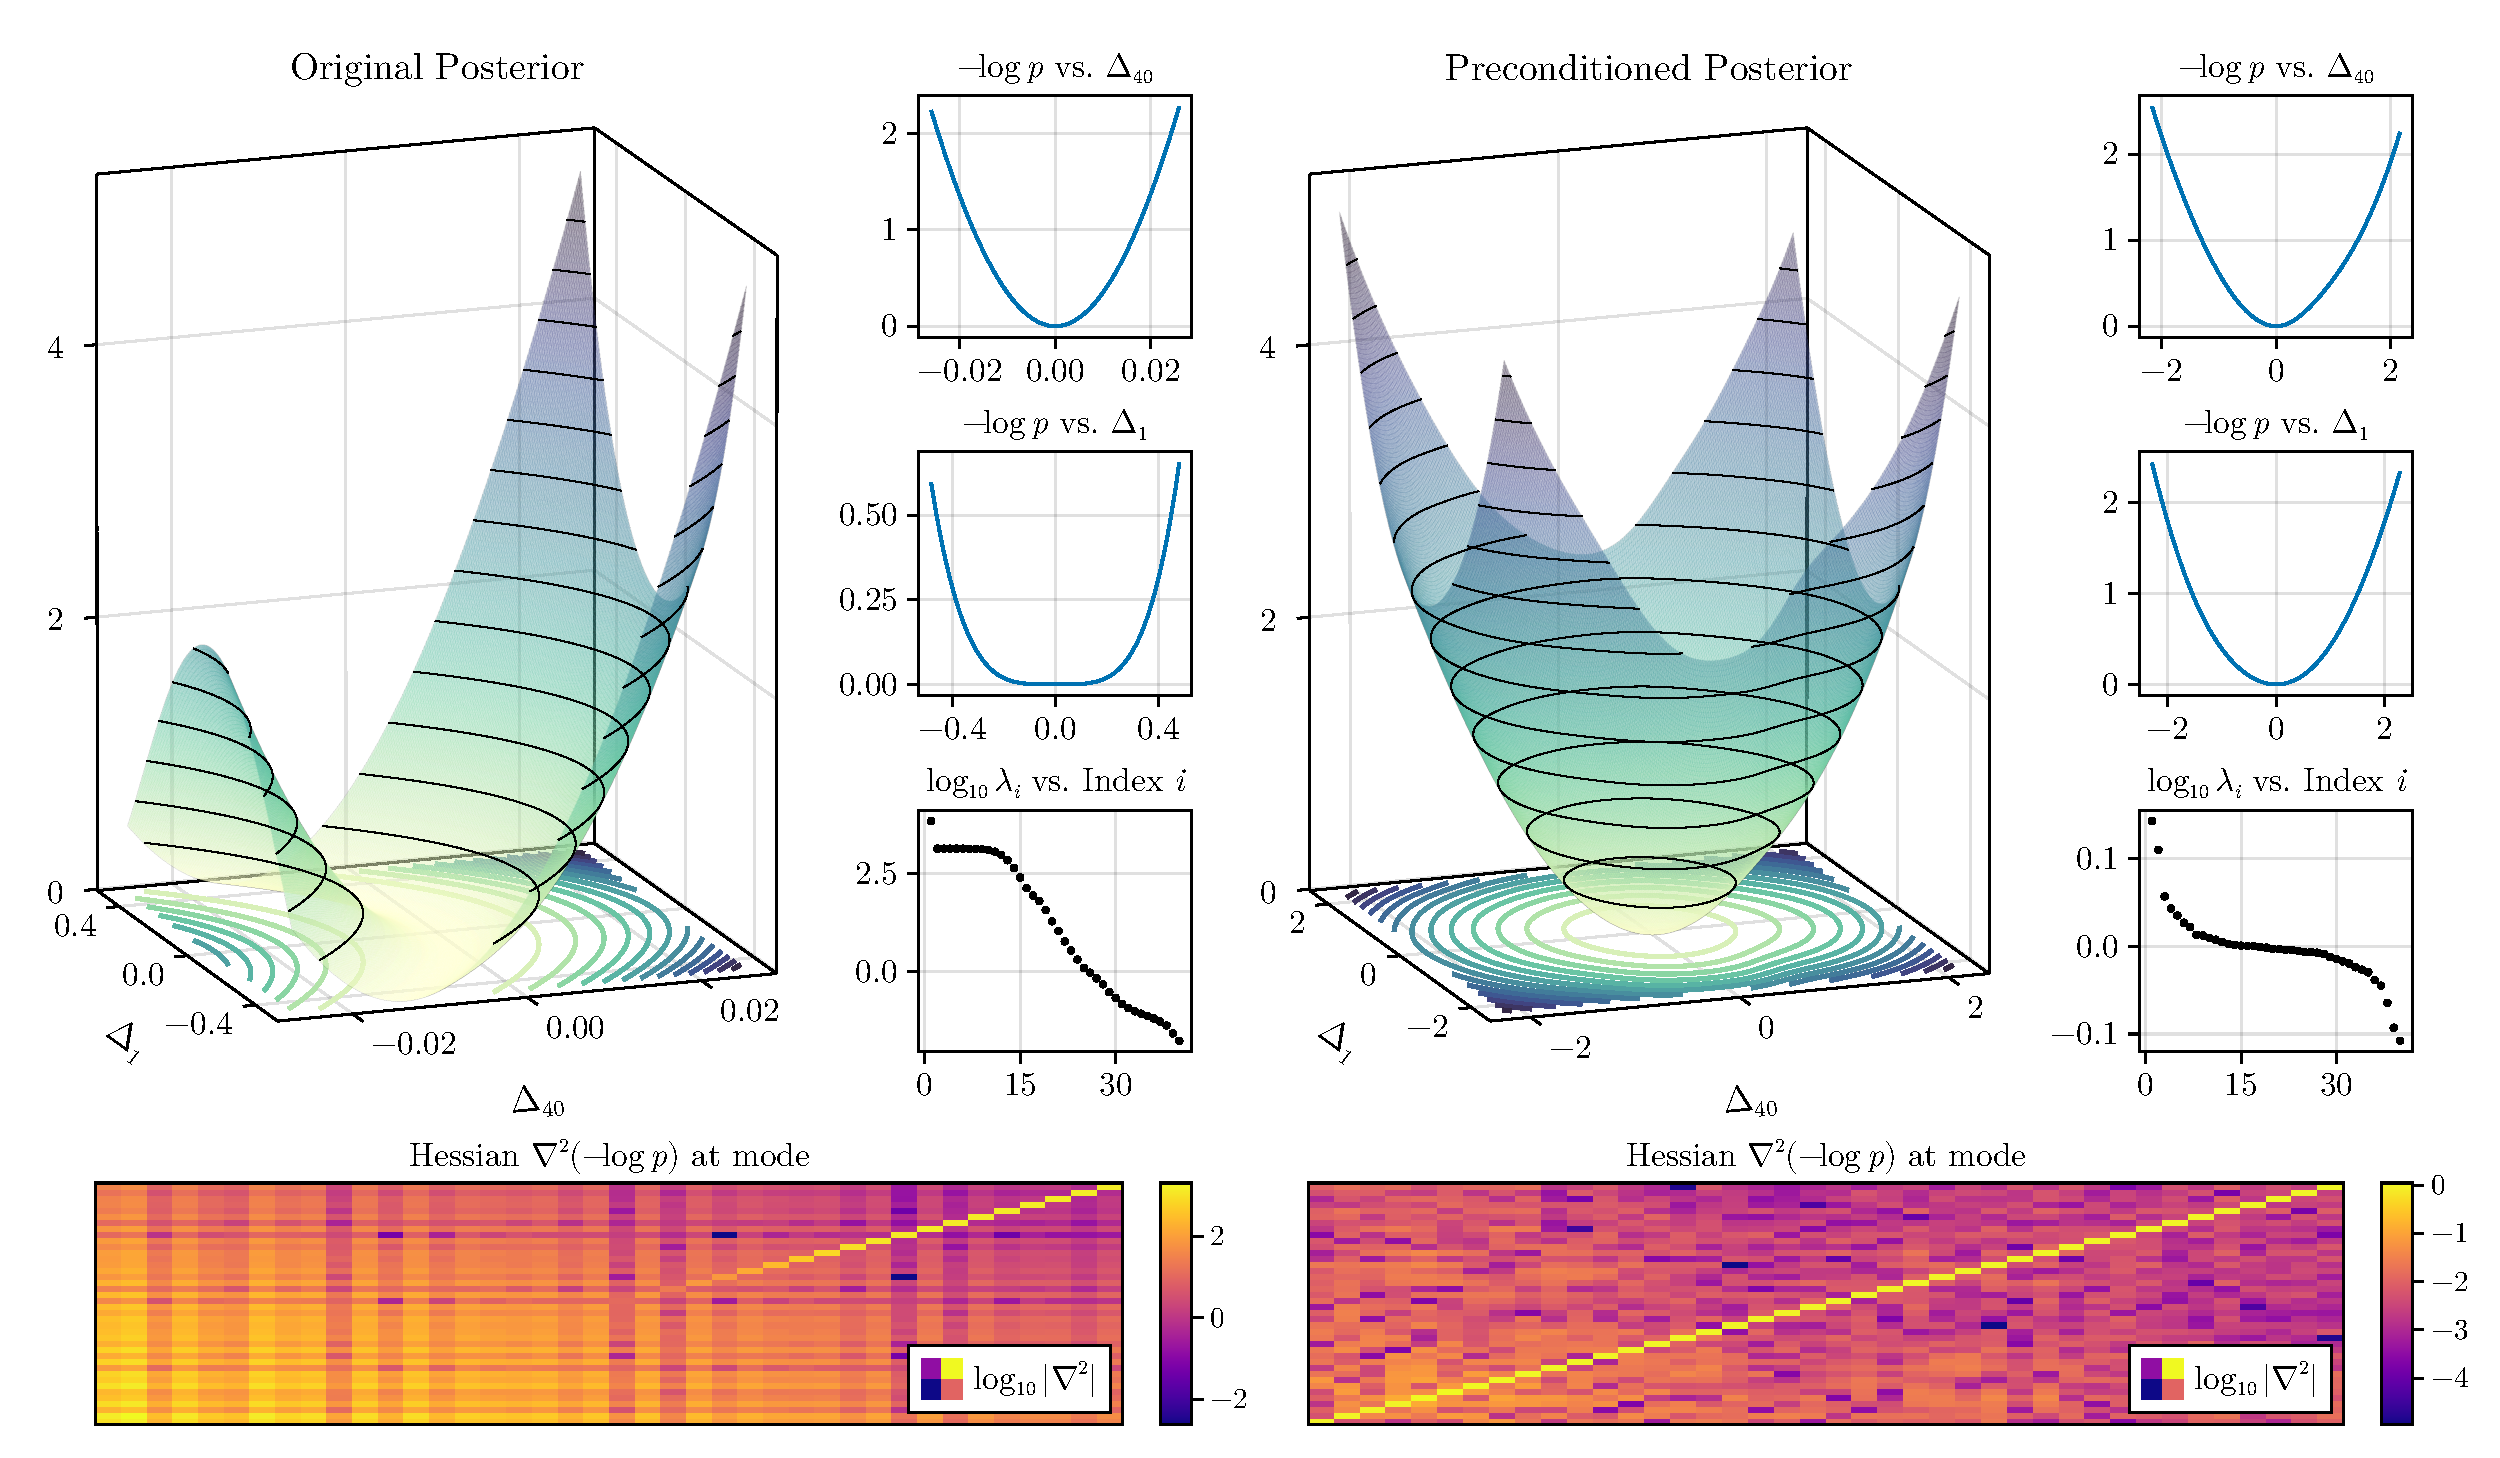
\includegraphics[width=\linewidth]{figures/preconditioning_geometry.pdf}
    \caption{Effect of the learned conditional normalizing flow preconditioner on the negative log-posterior at the \gls*{MAP} solution for a representative in vivo voxel.
    The columns differ only in that the right column uses the learned change of variables from~\cref{eqn:deep_distbn_sampling}, whereas the left column replaces the learned backbone $\varphi_{\vv{\xi}}$ with the identity.
    Within each column, the surface plot shows the posterior surface, recentred to the mode $u_{\bar{\distbn}}^*$, spanned by the Hessian eigenvectors corresponding to the largest and smallest eigenvalues, $\vv{u}_{\bar{\distbn}} = u_{\bar{\distbn}}^* + \Delta_{1} \hat{e}_{1} + \Delta_{n_{T_2}-1} \hat{e}_{n_{T_2}-1}$, with nuisance dimensions $\vv{u}_{\eta} = 0$ fixed at the mode;
    the three smaller panels show the negative log-posterior profiles along each axis through the origin, as well as the sorted eigenvalue spectrum $\log_{10}\lambda_i$;
    and the bottom panel shows the log-absolute Hessian values $\log_{10}|\nabla^2(-\log p)|$ at the mode.
    The trained flow produces a posterior geometry that is approximately an isotropic quadratic bowl.}
    \label{fig:preconditioning_geometry}
\end{figure}

\subsubsection{Conditional Normalizing Flows}

Let $q_{\bar{\distbn}}$ be a conditional density defined by
\begin{align}
    \log q_{\bar{\distbn}}(\bar{\distbn} \mid \signal)               & = \log \pi_{\vv{u}}(\vv{u}) - \log \AbsDet{\vv{J}_{\varphi_{\bar{\distbn}}}(\vv{u}; \signal)}, \label{eqn:norm_flow_density}                     \\
    \bar{\distbn} \sim q_{\bar{\distbn}}(\bar{\distbn} \mid \signal) & \Leftrightarrow \bar{\distbn} = \varphi_{\bar{\distbn}}(\vv{u}; \signal) \text{ where } \vv{u} \sim \pi_{\vv{u}}. \label{eqn:norm_flow_sampling}
\end{align}
We say that the \textit{flow} $\varphi_{\bar{\distbn}}$, a diffeomorphism, \textit{pushes forward} samples $\vv{u}$ drawn from the \textit{base distribution} $\pi_{\vv{u}}$ to samples $\bar{\distbn} \sim q_{\bar{\distbn}}$;
we thus refer to $q_{\bar{\distbn}} = \varphi_{\bar{\distbn}} \circ \pi_{\vv{u}}$ as the \textit{pushforward} density of $\pi_{\vv{u}}$ by $\varphi_{\bar{\distbn}}$.
If we let $\pi_{\vv{u}} = \mathcal{N}(\Zero, \Id_{n_{T_2}-1})$\footnote{The dimension of the base distribution $\pi_{\vv{u}}$ must match the degrees of freedom of $\bar{\distbn}$ (constrained by $\sum_{i} \bar{\distbn}_i = 1$) for the flow to be invertible.},
we see from~\eqref{eqn:density_change_of_vars} and~\eqref{eqn:norm_flow_density} that if $q_{\bar{\distbn}}$ approximates the marginal posterior $p(\bar{\distbn} \mid \signal)$, then the \textit{inverse flow} $\varphi_{\bar{\distbn}}^{-1}$ will approximately \textit{normalize} the posterior:
\begin{align*}
    p(\bar{\distbn} \mid \signal) \approx q_{\bar{\distbn}}(\bar{\distbn} \mid \signal) \Rightarrow p(\vv{u} \mid \signal) = \varphi_{\bar{\distbn}}^{-1}(\cdot; \signal) \circ p(\bar{\distbn} \mid \signal) \approx \pi_{\vv{u}}(\vv{u}),
\end{align*}
hence the name (conditional) \textit{normalizing} flow.
Note that it is this property that makes $\varphi_{\bar{\distbn}}^{-1}$ a powerful preconditioner for sampling;
the complexities of $p(\bar{\distbn} \mid \signal)$ are smoothed away by $\varphi_{\bar{\distbn}}^{-1}$, resulting in a posterior surface with much simpler geometry: $-\log p(\vv{u} \mid \signal) \approx \frac{1}{2} \lVert \vv{u} \rVert^2 + C$ (see \cref{fig:preconditioning_geometry}).
Furthermore, the flow need not be perfectly trained (impossible in practice) to see benefits;
any improvements in the posterior geometry will help downstream inference in $\vv{u}$-space.

The base distribution $\pi_{\vv{u}}$ can be transformed into an arbitrarily complex density $q_{\bar{\distbn}}$ by $\varphi_{\bar{\distbn}}$,
and so normalizing flows can be seen as a generalization of the \textit{reparameterization trick}: the sampling procedure \eqref{eqn:norm_flow_sampling} can be differentiated by caching $\vv{u} \sim \pi_{\vv{u}}$ during the forward pass of the backpropagation algorithm and then differentiating through $\varphi_{\bar{\distbn}}$ as usual.
It is furthermore crucial in practice that flows are \textit{composable}: given $L$ diffeomorphisms $\{\varphi_{\bar{\distbn}, i}\}_{i=1}^{L}$, the function composition $\varphi_{\bar{\distbn}} = \varphi_{\bar{\distbn}, L} \circ \cdots \circ \varphi_{\bar{\distbn}, 1}$ is itself a diffeomorphism which transforms $\pi_{\vv{u}}$ into $q_{\bar{\distbn}}$ such that
\begin{align}\label{eqn:norm_flow_density_sum}
    \log q_{\bar{\distbn}}(\bar{\distbn} \mid \signal)
    = \log \pi_{\vv{u}}(\vv{u})
    - \sum_{i=1}^{L}
    \log \AbsDet{\vv{J}_{\varphi_{\bar{\distbn}, i}}(\vv{u}_{i-1}; \signal)},
\end{align}
where $\vv{u}_{i} = \varphi_{\bar{\distbn}, i}(\vv{u}_{i-1}; \signal)$, $\vv{u}_{0} = \vv{u}$, $\vv{u}_{L} = \bar{\distbn}$, and $\vv{J}_{\varphi_{\bar{\distbn}, i}}$ is the Jacobian of $\varphi_{\bar{\distbn}, i}$ at $\vv{u}_{i-1}$.
Invertibility follows from $\varphi_{\bar{\distbn}}^{-1} = \varphi_{\bar{\distbn}, 1}^{-1} \circ \cdots \circ \varphi_{\bar{\distbn}, L}^{-1}$.

\subsubsection{Flow Architecture}\label{subsubsec:flow_architecture}

The conditional normalizing flow $\varphi_{\bar{\distbn}}$ is composed of $B$ flow blocks, the low-pass window $\Lambda$ of \cref{subsubsec:shallow_prior}, and an inverse \gls*{ILR} transform:
\begin{align}
    \varphi_{\bar{\distbn}} = \InvILR{\cdot; \beta_{0}} \circ \Lambda \circ \varphi_{\text{block}}^{(B)} \circ \cdots \circ \varphi_{\text{block}}^{(1)}.
\end{align}
Each block has the form:
\begin{align}\label{eqn:flow_block}
    \varphi_{\text{block}} = E \circ T^{-1} \circ C \circ T,
\end{align}
where $T$ denotes an affine linear flow, $C$ a symmetric affine coupling flow, and $E$ an elementwise affine flow.
The block structure derives from the real-NVP family of architectures~\citep{dinh_density_2017,dinh_nice_2015,kingma_glow_2018,prenger_waveglow_2019}, with a slight modification inspired by Fourier neural operators~\citep{li_fourier_2021}, where the learned affine flow $T$ replaces the Fourier transform.
Each block applies four transformations:
(1) linearly transform \gls*{ILR} coefficients to a learned space, allowing global interactions between dimensions;
(2) apply the nonlinear symmetric coupling flow $C$;
(3) linearly transform back to \gls*{ILR} space via $T^{-1}$; and
(4) apply an elementwise affine transformation $E$ in \gls*{ILR} space.
See \cref{fig:flow_diagram} for the factored joint flow and \cref{fig:architecture}(b) for the backbone block structure.

\begin{figure}[ht]
    \centering
    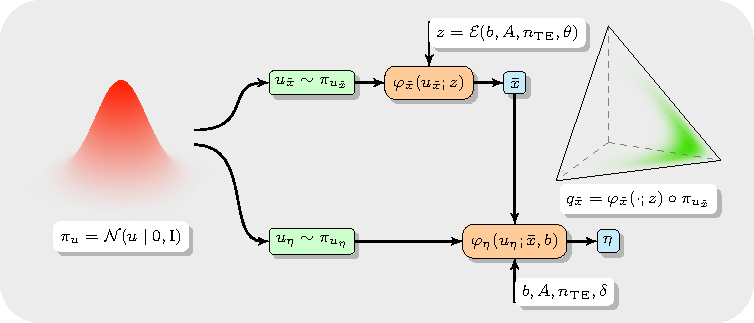
\includegraphics[width=\linewidth]{figures/flow-diagram.pdf}
    \caption{Factored conditional normalizing flow architecture.
        A deep flow $\varphi_{\bar{\distbn}}$ is trained to approximate the marginal posterior $p(\bar{\distbn} \mid \signal)$ over the normalized $T_2$ distribution, while the conditional posterior $p(\eta \mid \bar{\distbn}, \signal)$ implements Laplace's approximation over the nuisance parameters $\eta = (\log s, \log \sigma)$ via the affine flow $\varphi_{\eta}$.}
    \label{fig:flow_diagram}
\end{figure}

For simplicity, we assume the number of $T_2$ components $n_{T_2}$ is odd, ensuring the spectrum-coordinate dimension $d = n_{T_2} - 1$ is even\footnote{Matrix multiplications within $\varphi_{\text{block}}$ are typically faster with even-dimensional vectors, too.}.

To condition the flow on the data, $C$ and $E$ also take an encoding vector $\latents \in \mathbb{R}^{n_{\latents}}$ as input, produced by a transformer-style encoder~\citep{vaswani_attention_2017}.
The measured signal $\signal$ and its projection $\epgbases^T\signal$ are encoded alongside \gls*{MRI}-specific data:
the quantization level $\delta$, the echo spacing $\TE$, the number of echoes $n_{\TE}$, the \gls*{EPG} matrix $\epgbases$, and the parameters defining $A$ (longitudinal $T_1$, transverse range $T_2^{\min}$ and $T_2^{\max}$, and flip angle $\alpha$).
The continuous parameters are formed into a vector $\theta$, where
\begin{align}\label{eqn:scalar_features}
    \theta_{0} = ( \delta, \log\delta, \cos\alpha, \sin\alpha, \tau_{2,1}, \tau_{2,2}, \log\tau_{2,1}, \log\tau_{2,2}, \tau_{1}, \log\tau_{1} ),
    \quad
    \theta = \frac{\theta_{0} - \mu_{\theta_{0}}}{\sigma_{\theta_{0}}},
\end{align}
$\tau_{2,1} = T_2^{\min} / \TE$, $\tau_{2,2} = T_2^{\max} / \TE$, $\tau_{1} = T_1 / \TE$,
and $\theta$ equals $\theta_{0}$ standardized to zero mean and unit variance using fixed (augmented-)training data statistics $\mu_{\theta_{0}}$ and $\sigma_{\theta_{0}}$.

\Cref{fig:architecture}(a) illustrates the encoder architecture.
The number of echoes $n_{\TE}$ is treated as a discrete token and input to the encoder via an embedding layer.
The token dimension is $n_{\mathrm{tok}} = 64$ and the \gls*{MLP} hidden dimension $4 n_{\mathrm{tok}} = 256$.
Sinusoidal positional encodings are added separately to the $4$ query tokens and the $4 + n_{T_2}$ key/value tokens.
A stack of $L = 2$ cross-attention transformer blocks with $8$ heads is applied sequentially to the query tokens;
the transformed queries are then mapped from $\mathbb{R}^{4 \times n_{\mathrm{tok}}}$ to $\latents_0 \in \mathbb{R}^{n_{\latents}}$, with $n_{\latents} = 128$, and a final RMSNorm layer projects $\latents_0$ to the sphere of radius $r = \sqrt{n_{\latents}}$, giving $\latents \in S_{r}^{n_{\latents} - 1}$.
These encoding vectors are regularized during training using the Wasserstein-2 regularizer described in \cref{subsubsec:encoder_regularization}.

\begin{figure}[ht]
    \centering
    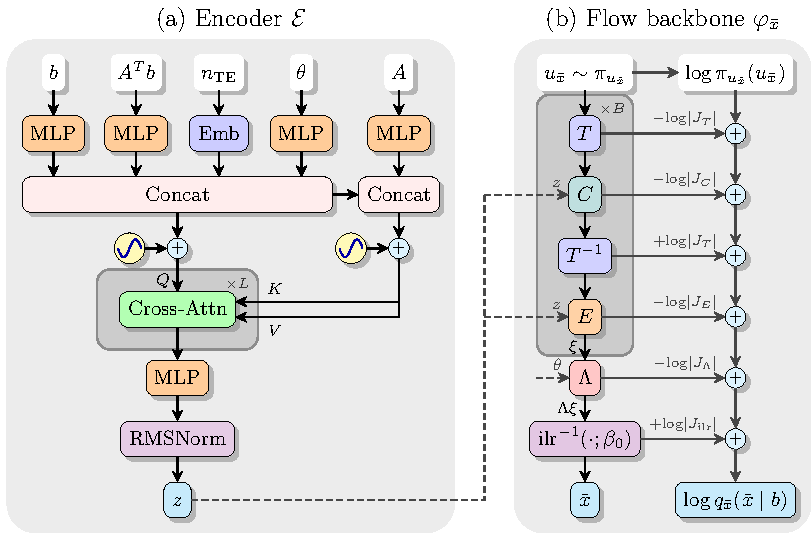
\includegraphics[width=0.7\linewidth]{figures/arch.pdf}
    \caption{Network architecture.
    (a) The encoder architecture, mapping the tokenized signal and scan parameters to the encoding vector $\latents \in S_{r}^{n_{\latents} - 1}$ via cross-attention.
    (b) The flow backbone architecture, pushing a base sample $\vv{u}_{\bar{\distbn}} \sim \mathcal{N}(\Zero, \Id)$ through the $B$ flow blocks, low-pass window $\Lambda$, and inverse \gls*{ILR} transform to produce a normalized $T_2$ distribution sample $\bar{\distbn}$.}
    \label{fig:architecture}
\end{figure}

The affine linear flow $T$ is parameterized using a matrix exponential:
\begin{align}\label{eqn:affine_flow}
    T\vv{u} = \exp(M)\vv{u} + \vv{c}, \qquad
    T^{-1}\vv{v} = \exp(-M)(\vv{v}-\vv{c}),
\end{align}
where $M\in\mathbb{R}^{d\times d}$ and $\vv{c}\in\mathbb{R}^{d}$, with $d=n_{T_2}-1$.
This parameterization is invertible for every finite $M$, with log-Jacobian determinant $\operatorname{tr}(M)$.
The inverse $T^{-1}$ shares parameters with $T$.

The elementwise affine flow $E$ scales and shifts each \gls*{ILR} coefficient independently as:
\begin{align}\label{eqn:elementwise_flow}
    \vv{u}' = \vv{s}\odot\vv{u} + \vv{t}, \;
    (\vv{a}, \vv{t}) = f_{E}(\latents), \quad \vv{s}=h(\vv{a}),
\end{align}
where $f_E : \mathbb{R}^{n_{\latents}} \to \mathbb{R}^{d} \times \mathbb{R}^{d}$ is an \gls*{MLP}.
The positive scale activation is $h(a)=(a+\sqrt{a^2+4})/2$, applied elementwise in both $E$ and $C$.
The log-Jacobian determinant for~\eqref{eqn:elementwise_flow} is
\begin{align}
    \log\AbsDet{\vv{J}_{E}(\vv{u}, \latents)} = \sum_{i}\log\vv{s}_i.
\end{align}
The symmetric coupling flow $C$ is composed of two coupling flows.
The input $\vv{u}$ is split in half into $\vv{u}_{1}$ and $\vv{u}_{2}$, and $\vv{u}$ is transformed one half at a time:
\begin{align}\label{eqn:symmetric_flow}
    \begin{split}
        \vv{u}_{1}^{\prime} = \vv{s}_{1} \odot \vv{u}_{1} + \vv{t}_{1}, \; (\vv{a}_{1}, \vv{t}_{1}) = f_{C_1}(\latents, \vv{u}_{2}), \quad \vv{s}_{1}=h(\vv{a}_{1}) \\
        \vv{u}_{2}^{\prime} = \vv{s}_{2} \odot \vv{u}_{2} + \vv{t}_{2}, \; (\vv{a}_{2}, \vv{t}_{2}) = f_{C_2}(\latents, \vv{u}_{1}^{\prime}), \quad \vv{s}_{2}=h(\vv{a}_{2})
    \end{split}
\end{align}
where $f_{C_1}, f_{C_2}: \mathbb{R}^{n_{\latents}} \times \mathbb{R}^{d/2} \to \mathbb{R}^{d/2} \times \mathbb{R}^{d/2}$ are \gls*{MLP}s.
The log-Jacobian determinant for~\eqref{eqn:symmetric_flow} is:
\begin{align}
    \log\AbsDet{\vv{J}_{C}(\vv{u}, \latents)} = \sum_{i}\log(\vv{s}_{1})_{i} + \sum_{i}\log(\vv{s}_{2})_{i}.
\end{align}

\subsubsection{Joint Flow for Posterior Approximation}\label{subsubsec:laplace_flow_nuisance}

In \cref{subsubsec:laplace_approximation}, we introduced Laplace's approximation $q_{\eta}$ to $p(\eta \mid \bar{\distbn}, \signal)$ for the nuisance parameters $\eta = (\log s, \log \sigma)$.
Since $q_{\eta}$ is Gaussian, it is equivalent to the pushforward of $\pi_{\vv{u}_{\eta}} = \mathcal{N}(\Zero, \Id_2)$ by an \textit{affine flow} $\varphi_{\eta}$ conditional on $\bar{\distbn}$ and $\signal$:
\begin{align}\label{eqn:laplace_flow}
    \begin{split}
        q_{\eta}(\eta \mid \bar{\distbn}, \signal)                & = \varphi_{\eta}(\cdot; \bar{\distbn}, \signal) \circ \pi_{\vv{u}_{\eta}} \\
        \varphi_{\eta}(\vv{u}_{\eta}; \bar{\distbn}, \signal) & = \mu_{\eta} + \Sigma_{\eta}^{1/2}\vv{u}_{\eta}
    \end{split}
\end{align}
where $\mu_{\eta}$ and $\Sigma_{\eta}$ are the mean and covariance of $q_{\eta}(\eta \mid \bar{\distbn}, \signal)$ computed via~\eqref{eqn:laplace_mean} and~\eqref{eqn:laplace_cov}.
Since $\Sigma_{\eta}$ is positive definite at $\mu_{\eta}$, $\varphi_{\eta}$ is a diffeomorphism with Jacobian $\Sigma_{\eta}^{1/2}$.

The Laplace flow $\varphi_{\eta}$ can be neatly integrated with the deep normalizing flow $\varphi_{\bar{\distbn}}$.
Let $\pi_{\vv{u}} = \pi_{\vv{u}_{\bar{\distbn}}} \times \pi_{\vv{u}_{\eta}} \cong \mathcal{N}(\Zero, \Id_{n_{T_2}+1})$ be the product of the base distributions $\pi_{\vv{u}_{\bar{\distbn}}} = \mathcal{N}(\Zero, \Id_{n_{T_2}-1})$ and $\pi_{\vv{u}_{\eta}} = \mathcal{N}(\Zero, \Id_{2})$.
Then, $q(\bar{\distbn}, \eta \mid \signal) = q_{\bar{\distbn}}(\bar{\distbn} \mid \signal) q_{\eta}(\eta \mid \bar{\distbn}, \signal)$ is the pushforward density $q = \varphi(\cdot; \signal) \circ \pi_{\vv{u}}$ with $\varphi$ given by
\begin{align}\label{eqn:joint_flow}
    \varphi(\vv{u}; \signal) & = (\bar{\distbn}, \eta)
    \text{ where }
    \begin{cases}
        \bar{\distbn} & = \varphi_{\bar{\distbn}}(\vv{u}_{\bar{\distbn}}; \signal) \\
        \eta          & = \varphi_{\eta}(\vv{u}_{\eta}; \bar{\distbn}, \signal)
    \end{cases}
\end{align}
and $\vv{u} = (\vv{u}_{\bar{\distbn}}, \vv{u}_{\eta})$.
Since $\bar{\distbn}$ does not depend on $\vv{u}_{\eta}$, the Jacobian $J_{\varphi}$ of $\varphi$ with respect to $\vv{u}$ is block-triangular with $J_{\varphi_{\bar{\distbn}}}$ and $J_{\varphi_{\eta}} = \Sigma_{\eta}^{1/2}$ on the diagonal.
Therefore, the update rule for the pushforward $q = \varphi(\cdot; \signal) \circ \pi_{\vv{u}}$ is given by:
\begin{align}\label{eqn:joint_flow_density}
    \begin{split}
        \log q(\bar{\distbn}, \eta \mid \signal)          & = \log \pi_{\vv{u}}(\vv{u}) - \log \AbsDet{\vv{J}_{\varphi}(\vv{u}; \signal)},                                 \\
        \log \AbsDet{\vv{J}_{\varphi}(\vv{u}; \signal)} & = \log \AbsDet{\vv{J}_{\varphi_{\bar{\distbn}}}(\vv{u}_{\bar{\distbn}}; \signal)} + \frac{1}{2} \log \AbsDet{\Sigma_{\eta}}.
    \end{split}
\end{align}

\subsection{Training}

\subsubsection{Variational Inference}\label{subsubsec:variational_inference}

We train the joint flow $\varphi$ in~\eqref{eqn:joint_flow} using amortized variational inference~\citep{kingma_auto-encoding_2014,rezende_stochastic_2014,rezende_variational_2016,papamakarios_normalizing_2021}.
For the approximate posterior $q = \varphi(\cdot; \signal) \circ \pi_{\vv{u}}$ from~\eqref{eqn:joint_flow_density}, the evidence lower bound (\gls*{ELBO}) is given by:
\begin{align}\label{eqn:evidence_lower_bound}
    \begin{split}
        \log p(\signal) & \ge \mathbb{E}_{q} \bigl[ \log p(\signal, \bar{\distbn}, \eta) - \log q(\bar{\distbn}, \eta \mid \signal) \bigr]                                             \\
        & = \mathbb{E}_{q} \bigl[ \log p(\signal \mid \bar{\distbn}, \eta) \bigr] - \KL \bigl[ q(\bar{\distbn}, \eta \mid \signal) \,\big\|\, p(\bar{\distbn}, \eta) \bigr] \\
        & = \mathbb{E}_{q} \bigl[ \log p(\signal, \bar{\distbn}, \eta) \bigr] + \mathcal{H} \bigl( q(\bar{\distbn}, \eta \mid \signal) \bigr)
    \end{split}
\end{align}
where $\KL[q \,\|\, p] = \mathbb{E}_{q} [ \log \frac{q}{p} ]$ is the \textit{Kullback--Leibler (\gls*{KL}) divergence} and $\mathcal{H}[q] = \mathbb{E}_{q}[-\log q]$ is the \textit{differential entropy}.
Maximizing the \gls*{ELBO} in~\eqref{eqn:evidence_lower_bound} has three equivalent interpretations:
(1) maximize the likelihood of the data while keeping $q$ close to the prior;
(2) maximize both the joint probability of the data and the entropy of $q$; and
(3) minimize $\KL [ q(\bar{\distbn}, \eta \mid \signal) \,\|\, p(\bar{\distbn}, \eta \mid \signal)  ]$ between $q$ and the true posterior\footnote{To see this, subtract $\log p(\signal)$ from both sides of~\eqref{eqn:evidence_lower_bound} and use Bayes' rule.}.

While the \gls*{KL} divergence and entropy have closed forms for Gaussian base distributions $\pi_{\vv{u}}$, a fully Monte Carlo estimate of the \gls*{ELBO} has lower variance when $q$ approaches the true posterior~\citep{roeder_sticking_2017}.
We therefore use the first form of the \gls*{ELBO} in~\eqref{eqn:evidence_lower_bound} and define the \textit{free energy} $\mathcal{F} [q]$ to be its negative.
In terms of $\varphi$, the free energy is given by:
\begin{align}\label{eqn:free_energy_joint_flow}
    \begin{split}
        \mathcal{F} [q] & = \mathbb{E}_{\pi_{\vv{u}}} \left[ \log q(\bar{\distbn}, \eta \mid \signal) - \log p(\signal, \bar{\distbn}, \eta) \right]                                      \\
        & = \mathbb{E}_{\pi_{\vv{u}}} \left[ \log \pi_{\vv{u}}(\vv{u}) - \log \AbsDet{\vv{J}_{\varphi}(\vv{u}; \signal)} - \log p(\signal, \bar{\distbn}, \eta) \right]
    \end{split}
\end{align}
where $(\bar{\distbn}, \eta) = \varphi(\vv{u}; \signal)$.
Given a dataset $\{\signal\}$ with empirical distribution $\tilde{p}(\signal)$, the objective is to minimize the free energy:
\begin{align}\label{eqn:free_energy_objective}
    \mathcal{L}_{\text{free}} = \mathbb{E}_{\tilde{p}} \left[ \mathcal{F} [q] \right] \text{ where } q = \varphi(\cdot; \signal) \circ \pi_{\vv{u}}.
\end{align}
Training optimizes the encoder, flow backbone, shared low-pass window, and nuisance-prior parameters;
the nuisance Laplace approximation has no trainable parameters.

\subsubsection{Path Gradient}

To reduce the variance of mini-batch gradient estimates of the free energy, especially as $q$ approaches the true posterior, we use the \textit{path gradient}~\citep{roeder_sticking_2017,agrawal_advances_2020,vaitl_fast_2024}:
\begin{align}\label{eqn:path_gradient}
    \blacktriangledown_{\phi} f(T(u; \phi), \phi) \coloneqq \left( \nabla_{\phi} f(T(u; \phi), \phi^\prime) \right)_{\phi^\prime = \phi}
\end{align}
where $f$ is a function of the output of the flow $T$ and its parameters $\phi$;
$\blacktriangledown_{\phi} f$ treats $f$ as a constant function of $\phi$, only accumulating gradients through the flow ``path'' $T(u; \phi)$.
Let the flow $\varphi$ in~\eqref{eqn:free_energy_joint_flow} have parameters $\phi$, and let $\StopGradient$ denote the stop-gradient which holds $\phi$ constant with respect to $\nabla_{\phi}$.
Then, $\blacktriangledown_{\phi} \log \frac{q}{p} = \nabla_\phi \log \frac{q_{\StopGradient}}{p}$, and we have
\begin{align}\label{eqn:path_gradient_free_energy}
    \blacktriangledown_{\phi} \mathcal{F}[q] = \mathbb{E}_{\pi_{\vv{u}}} \left[\nabla_{\phi} \left( \log q_{\StopGradient}(\bar{\distbn}, \eta \mid \signal) - \log p(\signal, \bar{\distbn}, \eta) \right) \right].
\end{align}
The reduced finite-sample variance of~\eqref{eqn:path_gradient_free_energy} comes at the cost of evaluating both the forward flow for $(\bar{\distbn}, \eta) = \varphi(\vv{u}; \signal)$ and the inverse flow for $\log\AbsDet{\vv{J}_{\varphi^{-1}_{\StopGradient}}}$.
Note that~\eqref{eqn:path_gradient_free_energy} is an unbiased estimate of the total gradient, i.e.\ $\blacktriangledown_{\phi}\mathcal{F}[q] = \nabla_{\phi}\mathcal{F}[q]$, since the \textit{score} satisfies $\mathbb{E}_{q}[\frac{\partial}{\partial\phi} \log q] = 0$.

\subsubsection{Self-Supervised Regularization}

We regularize the flow $q(\bar{\distbn}, \eta \mid \signal)$ using synthetic data.
First, labels $(\bar{\distbn}, \eta) \sim p(\bar{\distbn}, \eta)$ are sampled from the prior.
Then, synthetic data $\signal \sim p(\signal \mid \bar{\distbn}, \eta)$ is simulated using the quantized Rician likelihood model~\eqref{eqn:signal_parameterization}.
The objective is to maximize the likelihood of the labels $(\bar{\distbn}, \eta)$ under $q$ conditioned on the simulated signal $\signal$:
\begin{align}\label{eqn:self_supervised_regularization}
    \mathcal{L}_{\text{self}} = \mathbb{E}_{p(\bar{\distbn}, \eta)} \mathbb{E}_{p(\signal \mid \bar{\distbn}, \eta)} \bigl[ -\log q(\bar{\distbn}, \eta \mid \signal) \bigr].
\end{align}
We use its marginal counterpart, supervising the spectrum posterior rather than the conditional nuisance approximation:
\begin{align}\label{eqn:self_supervised_regularization_marginal}
    \mathcal{L}_{\text{self}}^{\prime} = \mathbb{E}_{p(\bar{\distbn}, \eta)} \mathbb{E}_{p(\signal \mid \bar{\distbn}, \eta)} \bigl[ -\log q_{\bar{\distbn}}(\bar{\distbn} \mid \signal) \bigr].
\end{align}
The omitted nuisance term depends on the shared learned prior parameters, so the marginal objective is a deliberate choice rather than an equivalent joint objective.
Neither the prior nor likelihood sampling processes are differentiated;
the sampled labels and data are treated as fixed.
Evaluating $\mathcal{L}_{\text{self}}^{\prime}$ requires an additional encoding of $\signal$ and pushing of $\bar{\distbn}$ through the inverse marginal flow $\varphi_{\bar{\distbn}}^{-1}$.

For a fixed prior and signal model, minimizing $\mathcal{L}_{\text{self}}^{\prime}$ minimizes the expected forward \gls*{KL} divergence between the marginal spectrum posteriors, since
\begin{align*}
    \mathcal{L}_{\text{self}}^{\prime} & = \mathbb{E}_{p(\signal)} \, \mathcal{H}\!\left[p(\bar{\distbn} \mid \signal),q_{\bar{\distbn}}(\bar{\distbn} \mid \signal)\right] \\
                                       & = \mathbb{E}_{p(\signal)} \, \KL\!\left[p(\bar{\distbn} \mid \signal) \,\|\, q_{\bar{\distbn}}(\bar{\distbn} \mid \signal)\right]
    + \mathbb{E}_{p(\signal)} \, \mathcal{H}\!\left[p(\bar{\distbn} \mid \signal)\right].
\end{align*}
The entropy term is independent of $q_{\bar{\distbn}}$ under this fixed model.
This marginal forward \gls*{KL} encourages $q_{\bar{\distbn}}$ to cover spectrum-posterior modes, complementing the reverse-\gls*{KL} free-energy objective~\eqref{eqn:free_energy_joint_flow}.

\subsubsection{Encoder Regularization}\label{subsubsec:encoder_regularization}

Regularizing the encoder outputs $\latents \in \mathbb{R}^{n_{\latents}}$ is necessary to ensure stable representations and prevent overfitting.
A common approach is $\ell^2$-regularization, equivalent to an i.i.d.\ unit normal prior on each $\latents_i$.
Inspired by VICReg~\citep{bardes_vicreg_2021}, we find that decorrelating $\latents$ components improves encodings.
We use half the squared Gaussian Wasserstein-2 distance:
\begin{gather}
    \mathcal{L}_{\text{enc}} = \tfrac12 \mathcal{W}_2^2(\mathcal{N}(\mu, \Sigma), \mathcal{N}(0, \Id)) = \sum_{i=1}^{n_{\latents}} \frac{\mu_i^2 + (\sqrt{\lambda_i} - 1)^2}{2} \label{eqn:w2_gaussian} \\
    \nabla_\mu \mathcal{L}_{\text{enc}} = \mu, \quad \nabla_\Sigma \mathcal{L}_{\text{enc}} = \frac{1}{2} (\Id - \Sigma^{-1/2}) \label{eqn:w2_gaussian_gradients}
\end{gather}
where $\mu, \Sigma$ are the mean and covariance of the encodings $\{ \latents^{j} \}$ of the current mini-batch of real and synthetic signals, and $\lambda_i$ are the eigenvalues of $\Sigma$.
Minimizing $\mathcal{L}_{\text{enc}}$ pushes $\mu \to 0$ and $\Sigma \to \Id$, whitening the components of $\latents$.

We find further improvement by normalizing encodings to unit \gls*{RMS} norm, i.e.\ $\lVert \latents \rVert_{\text{RMS}}^2 = \frac{1}{n_{\latents}}\lVert \latents \rVert_2^2 = 1$, constraining $\latents$ to the sphere $S_{r}^{n_{\latents} - 1}$ with radius $r = \sqrt{n_{\latents}}$.
The loss $\mathcal{L}_{\text{enc}}$ then encourages zero mean and identity covariance on this sphere.

\subsubsection{Training}\label{subsubsec:training_details}

Training consisted of $\num{160000}$ optimizer updates over approximately \SI{44}{\hour} on one NVIDIA Tesla V100 \gls*{GPU} with \SI{32}{GB} memory and six CPU threads on UBC ARC Sockeye~\citep{ubc_arc_sockeye}.
The full training objective is
\begin{align}\label{eqn:total_objective}
    \mathcal{L} = \mathcal{L}_{\text{free}} + \lambda_{\text{self}} \mathcal{L}_{\text{self}}^{\prime} + \lambda_{\text{enc}} \mathcal{L}_{\text{enc}},
\end{align}
combining the variational free energy~\eqref{eqn:free_energy_objective}, the self-supervised forward-\gls*{KL} loss~\eqref{eqn:self_supervised_regularization_marginal}, and the Wasserstein-2 encoding regularization~\eqref{eqn:w2_gaussian}.
The variational free energy is a reverse-\gls*{KL} objective over batches of measured data $\signal$, whereas the forward-\gls*{KL} loss requires batches of samples from the prior $p(\bar{\distbn}, \eta)$ and forward simulated synthetic data $\signal \sim p(\signal \mid \bar{\distbn}, \eta)$.
We use equal weighting $\lambda_{\text{self}} = 1$ throughout, encouraging the model to learn posteriors over both synthetic signals and real signals equally well.
The encoder weighting was also $\lambda_{\text{enc}} = 1$.

The flow and encoder were optimized using preconditioned stochastic gradient descent (\textsc{PSGD}) with Kronecker-factored triangular preconditioners~\citep{li_preconditioned_2018,li_stochastic_2025} and schedule-free momentum~\citep{defazio_road_2024,nestler_heavyball_2026}.
We use preconditioner learning rate $\eta_Q = 0.1$, update \gls*{RMS}-clip of $3$, schedule-free momentum with $\beta_1 = 0.99$, base learning rate $10^{-2}$, a linear warm-up from zero over $500$ optimizer steps, and decoupled weight decay $\lambda_{\mathrm{wd}} = 10^{-3}$ on dense weight matrices.

Training used a batch size of $\num{16384}$ with online data augmentation:
signals and their corresponding \gls*{EPG} rows were retained at a uniformly chosen ordered subset of $n'_{\TE}$ echoes, where $P(n'_{\TE}=n)\propto e^{\lambda n}$ for $n\in\{16,\ldots,56\}$ and $\lambda>0$ sets $\mathbb{E}[n'_{\TE}]=48$, then zero-padded;
quantized signals were uniformly dequantized and requantized using $\delta'=\delta Z$, where $Z$ is log-normal with mean $1$ and standard deviation $0.5$;
the \gls*{DECAES} flip-angle estimate $\alpha$ was perturbed by zero-mean Gaussian noise with standard deviation \SI{1}{\degree};
and $T_1$ and the $T_2$ range were randomized by drawing $T_2^{\min}$ uniformly from $[\TE - \SI{1}{\ms}, \TE + \SI{3}{\ms}]$ and $T_2^{\max}$ and $T_1$ uniformly from $[\SI{1}{s}, \SI{2}{s}]$.

\subsection{Inference}

Given a trained flow $\varphi$ and corresponding approximate posterior $q = \varphi(\cdot; \signal) \circ \pi_{\vv{u}}$, we must choose a posterior sampling method.
Even limiting ourselves to \gls*{MCMC} methods, there exists a dauntingly large literature of approaches to choose from~\citep{brooks_handbook_2011}.
For this reason, we consider an exhaustive comparison of \gls*{MCMC} methods beyond the scope of this work.
Instead, we compare three established, simple methods and leave the investigation of more advanced techniques for future work.

\paragraph*{(1) Direct and Importance-Weighted Sampling}

The simplest inference method samples directly from the approximate posterior $q(\bar{\distbn}, \eta \mid \signal)$.
This requires only a single forward pass through the flow per sample, but relies entirely on the model's generalization and may not fully capture the true posterior structure~\citep{dax_neural_2023}.
If only $\bar{\distbn}$ is needed, one can directly sample the marginal posterior $q_{\bar{\distbn}}(\bar{\distbn} \mid \signal)$.

Importance-weighted sampling reweights proposal samples using the importance weights:
\begin{align}\label{eqn:importance_sampling}
    \begin{cases}
        (\bar{\distbn}_{t}, \eta_{t}) \sim q(\bar{\distbn}, \eta \mid \signal), \\[6pt]
        w_{t} = \frac{p(\signal \mid \bar{\distbn}_{t}, \eta_{t}) p(\bar{\distbn}_{t}, \eta_{t})}{q(\bar{\distbn}_{t}, \eta_{t} \mid \signal)} \propto \frac{p(\bar{\distbn}_{t}, \eta_{t} \mid \signal)}{q(\bar{\distbn}_{t}, \eta_{t} \mid \signal)}.
    \end{cases}
\end{align}
Posterior expectations are then estimated as weighted averages,
\begin{align}\label{eqn:importance_sampling_expectation}
    \mathbb{E}_{p(\bar{\distbn}, \eta \mid \signal)}(f(\bar{\distbn}, \eta)) \approx \sum_{t=1}^T \tilde{w}_{t} f(\bar{\distbn}_{t}, \eta_{t}),
\end{align}
where $\tilde{w}_{t} = w_{t}/\sum_{t^\prime} w_{t^\prime}$.
The accuracy of importance sampling depends critically on the proposal distribution;
poorly matched proposals yield high-variance estimates~\citep{domke_importance_2018,muller_neural_2019}.
Neural networks have been used to improve proposals, though careful training is necessary to prevent mode-seeking behaviour~\citep{midgley_flow_2023}.

\paragraph*{(2) Metropolis--Hastings (\gls*{MH}) Algorithm}

Given an initial sample $\vv{u}_{0} \sim \pi_{\vv{u}}(\vv{u})$ and a \textit{proposal distribution} $Q(\tilde{\vv{u}} \mid \vv{u})$, a sequence $( \vv{u}_{t} )_{t \ge 1}$ of posterior samples is generated as follows~\citep{metropolis_equation_1953,hastings_monte_1970}:
\begin{align}\label{eqn:metropolis_hastings}
    \begin{cases}
        \tilde{\vv{u}} & \sim Q(\tilde{\vv{u}} \mid \vv{u}_{t})                                                                                                                                                                                                                                                                                                                                       \\
        A_t            & = \min \left\{ 1, \tfrac{p(\tilde{\vv{u}} \mid \signal)}{p(\vv{u}_{t} \mid \signal)} \tfrac{Q(\vv{u}_{t} \mid \tilde{\vv{u}})}{Q(\tilde{\vv{u}} \mid \vv{u}_{t})} \right\}                                                                                                                                                                                                   \\
                       & = \min \left\{ 1, \tfrac{p(\signal \mid \tilde{\bar{\distbn}}, \tilde{\eta})}{p(\signal \mid \bar{\distbn}_{t}, \eta_{t})} \tfrac{p(\tilde{\bar{\distbn}}, \tilde{\eta})}{p(\bar{\distbn}_{t}, \eta_{t})} \tfrac{| \det({\tilde{\vv{J}}_{\varphi}}) |}{| \det({\vv{J}_{\varphi,t}}) |} \tfrac{Q(\vv{u}_{t} \mid \tilde{\vv{u}})}{Q(\tilde{\vv{u}} \mid \vv{u}_{t})} \right\} \\
        \vv{u}_{t+1}   & = \tilde{\vv{u}} \text{ with probability } A_t, \text{ else } \vv{u}_{t}.
    \end{cases}
\end{align}
In the experiments below, \gls*{MH} uses the learned approximate posterior as an independent proposal distribution.
Equivalently, in $\vv{u}$-space we set $Q(\tilde{\vv{u}} \mid \vv{u}) = \mathcal{N}(\Zero, \Id)$, draw each proposed $\tilde{\vv{u}}$ from the base distribution, and map it through $\varphi$.
If $\varphi$ is well trained, then $q(\bar{\distbn}, \eta \mid \signal) \approx p(\bar{\distbn}, \eta \mid \signal)$ and the acceptance ratio is high.
If the approximation is poor, states with large target-to-proposal density ratios can be retained through repeated rejections.
Random-walk Metropolis (\gls*{RWM}) proposals such as $Q(\tilde{\vv{u}} \mid \vv{u}) = \mathcal{N}(\vv{u}, \sigma_{\mathrm{RWM}}^2 \Id)$ may also be used.

\paragraph*{(3) Metropolis-Adjusted Langevin Algorithm (\gls*{MALA})}

The unadjusted Langevin algorithm (\gls*{ULA})~\citep{bakry_diffusions_1985} generates posterior samples by performing noisy gradient ascent on the log-posterior starting from $\vv{u}_{0} \sim \pi_{\vv{u}}(\vv{u})$:
\begin{align}\label{eqn:langevin_dynamics_uspace}
    \vv{u}_{t+1} & = \vv{u}_{t} + \tau_{t} \nabla_{\vv{u}} \log p(\vv{u}_{t} \mid \signal) + \sqrt{2 \tau_{t}} \vvb{\xi}_{t},
\end{align}
where $\tau_{t}$ is the step size, and $\vvb{\xi}_{t}\sim\mathcal{N}(\Zero,\Id)$.
Under suitable regularity and decreasing-step-size conditions, the distribution of $\vv{u}_{t}$ approaches the stationary distribution $p(\vv{u} \mid \signal)$.
By Bayes' theorem, the gradient of the log-posterior can be exactly computed as
\begin{align}\label{eqn:langevin_dynamics_uspace_score}
    \begin{split}
        \nabla_{\vv{u}} \log p(\vv{u}_{t} \mid \signal) & = \nabla_{\vv{u}} (\log p(\bar{\distbn}_{t}, \eta_{t} \mid \signal) + \log\AbsDet{\vv{J}_{\varphi,t}}) \\
        & = \nabla_{\vv{u}} (\log p(\signal, \bar{\distbn}_{t}, \eta_{t}) + \log\AbsDet{\vv{J}_{\varphi,t}}).
    \end{split}
\end{align}
Langevin methods efficiently explore high-probability regions by leveraging gradient information, making them particularly effective in high dimensions compared to random walk Metropolis algorithms.
However, fixed step sizes $\tau_t = \tau$ generally introduce discretization bias in the stationary distribution~\citep{roberts_exponential_1996}.

The \textit{Metropolis-adjusted Langevin algorithm (\gls*{MALA})} corrects this issue by incorporating a Metropolis--Hastings accept-or-reject step~\citep{roberts_optimal_1998} using a proposal based on the \gls*{ULA}~\eqref{eqn:langevin_dynamics_uspace_score}:
\begin{align}
    \begin{cases}
        Q(\tilde{\vv{u}} \mid \vv{u}_{t}) & = \mathcal{N}(\vv{u}_{t} + \tau \nabla_{\vv{u}} \log p(\vv{u}_{t} \mid \signal), 2 \tau \Id) \\
        \vv{u}_{t+1}                      & = \text{Metropolis--Hastings step \eqref{eqn:metropolis_hastings}}.
    \end{cases}
\end{align}
For sufficiently regular product target distributions in the high-dimensional limit, \gls*{MALA} achieves an asymptotically optimal mean acceptance rate near $A \approx 0.574$~\citep{roberts_optimal_1998}.

\subsubsection{Flow Inference Implementation Details}\label{subsubsec:inference_details}

All sampling methods operate over the joint base-space coordinates $\vv{u} \in \mathbb{R}^{n_{\vv{u}}}$, with $n_{\vv{u}}=n_{T_2}+1$, using the learned flow $\varphi(\cdot; \signal)$ as a change of variables onto the joint parameter space over $(\bar{\distbn}, \eta)$, with one chain initialized at $\vv{u}_0 \sim \pi_{\vv{u}} = \mathcal{N}(\Zero, \Id)$ per voxel.

Because the trained flow approximately normalizes the base-space posterior in the sense that $p(\vv{u} \mid \signal) \approx \mathcal{N}(\Zero, \Id)$, the \gls*{RWM} and \gls*{MALA} proposal parameters may be set analytically using the constants derived for a standard normal target, rather than tuned:
we use the \gls*{RWM} proposal variance $\sigma_{\mathrm{RWM}}^2 = 2.382^2 / (n_{\vv{u}} - 1)$~\citep{roberts_weak_1997} and the \gls*{MALA} step size $\tau \approx 1.650^2 / (2\sqrt[3]{n_{\vv{u}}})$, equivalently a proposal standard deviation of $\sqrt{2\tau} \approx 1.650 / \sqrt[6]{n_{\vv{u}}}$~\citep{roberts_optimal_1998}.
The numerical scale factors are asymptotically optimal for standard normal target distributions, achieving the more generally optimal acceptance rates $A_{\text{\gls*{RWM}}}^* = 0.234$ and $A_{\text{\gls*{MALA}}}^* = 0.574$.

We report posterior means and central \SI{95}{\percent} credible intervals (\gls*{CI}s), summarized by their half-widths, for both $\bar{\distbn}$ and scalar biomarkers of interest:
the myelin (\gls*{MWF}), intra-/extracellular (\gls*{IEWF}), and cerebrospinal (\gls*{CWF}) water fractions, and the geometric mean $T_2$ over the full spectrum (GM $T_2$) and myelin-water pool (MW $T_2$).
Data is batched across voxels, computing encoder and flow quantities in parallel on the \gls*{GPU};
the exception is the no-U-turn sampler, which, due to dynamic chain lengths, was run on the \gls*{CPU} (see~\cref{subsec:preconditioning_ablation}).

\subsection{Joint Prior}\label{subsec:joint_prior}

The joint prior over the inference variables $(\bar{\distbn}, \eta)$ is taken to be factorized as
\begin{align}\label{eqn:joint_prior_factorization}
    p(\bar{\distbn}, \eta) = p(\bar{\distbn}) p(\log s) p(\log \sigma),
\end{align}
reflecting the modelling assumption that the normalized $T_2$ spectrum of the underlying tissue is approximately independent of the per-voxel signal scale and noise level.

\paragraph*{Low-Pass Prior on $\bar{\distbn}$.}
The prior on $\bar{\distbn}$ is given by the shallow low-pass distribution of~\cref{eqn:low_pass_prior}, obtained by pushing a standard Gaussian $\pi_{\vv{u}_{\bar{\distbn}}} = \mathcal{N}(\Zero, \Id)$ through a diagonal window filter $\Lambda = \Diag{\lambda_1^+, \ldots, \lambda_{n_{T_2}-1}^+}$ in \gls*{DCT} frequency space and then applying the inverse \gls*{ILR} transform.
We use a scaled Gaussian window
\begin{align}\label{eqn:gaussian_window}
    \lambda_i = \lambda_0 \exp\!\left( -(f_i / F_c)^2 / 2 \right),
\end{align}
where $f_i = i/n_{T_2}$ indexes the non-zero \gls*{DCT} frequency bins, $F_c > 0$ is a learnable cutoff, and $\lambda_0 > 0$ is a learnable amplitude.
Because the low-pass filtering is applied to \gls*{DCT} coefficients corresponding to $\log \bar{\distbn}$ over the $\log T_2$ grid (\cref{sec:apx:simplex_distributions_asymptotics}), $F_c$ is a cutoff \textit{in log-$T_2$ frequency}, and consequently, the learned width is scale-invariant in $T_2$:
altering $T_2^{\min}$ or $T_2^{\max}$ rescales the $\log T_2$ grid but does not change the relative smoothness of spectra favoured by the prior.
The amplitude $\lambda_0$ scales the low-passed coefficients, sharpening the $T_2$ peaks by increasing the amplitude of the logits as $\lambda_0$ grows, concentrating the softmax distribution.
A positive floor $\lambda_{\min} > 0$ is also added to $\lambda_i$ in quadrature via $\lambda_i^{+} = \sqrt{\lambda_i^2 + \lambda_{\min}^2}$ -- equivalent in distribution to adding isotropic Gaussian noise of variance $\lambda_{\min}^2$ in \gls*{ILR} space -- preventing complete attenuation of high-frequency components to zero.
This same window $\Lambda$ forms the terminal layer of the generator flow $\varphi_{\bar{\distbn}}$ such that the prior and the flow naturally reside in the same space of smooth $T_2$ spectra.

\paragraph*{Priors on $\eta = (\log s, \log \sigma)$.}
Both components of $\eta$ are assigned independent Gaussian priors.
The log-scale prior $p(\log s) = \mathcal{N}(\log s \mid \mu_{\log s, 0}, \sigma_{\log s, 0}^2)$ is initialized such that $\mathbb{E}[s] = 1$ and the scale is $s \approx 1 \pm 0.05$.
The log-noise prior $p(\log \sigma) = \mathcal{N}(\log \sigma \mid \mu_{\log \sigma, 0}, \sigma_{\log \sigma, 0}^2)$ is initialized with $\mu_{\log \sigma,0}=-30\log(10)/20$ and $\sigma_{\log \sigma,0}=10\log(10)/20$;
for $\mathrm{SNR}_{\si{\decibel}}=-20\log_{10}\sigma$, these values correspond to mean \SI{30}{\decibel} and standard deviation \SI{10}{\decibel}.
The hyperparameters $(\mu_{\eta,0}, \Sigma_{\eta,0})$, window cutoff $F_c$, amplitude $\lambda_0$, and floor $\lambda_{\min}$ (initialized at $0.1$) are learned jointly by approximate empirical Bayes during training, and the same nuisance priors are shared inside Laplace's approximation~\eqref{eqn:laplace_mean}.
At the final $\num{160000}$-update checkpoint, the learned window has $F_c=0.2093$ for $n_{T_2}=41$ over \SIrange{8}{1000}{\ms}, $\lambda_0=8.041$, and $\lambda_{\min}=0.02695$.
The learned Gaussian priors on $\log s$ and $\log\sigma$ have mean/standard-deviation pairs $(-0.002845,0.005426)$ and $(-5.6575,0.6774)$, respectively.
Using fixed floors between $0.025$ and $0.4$ changed the held-out free energy by approximately $0.01$ nats per voxel.

\begin{figure}[ht]
    \centering
    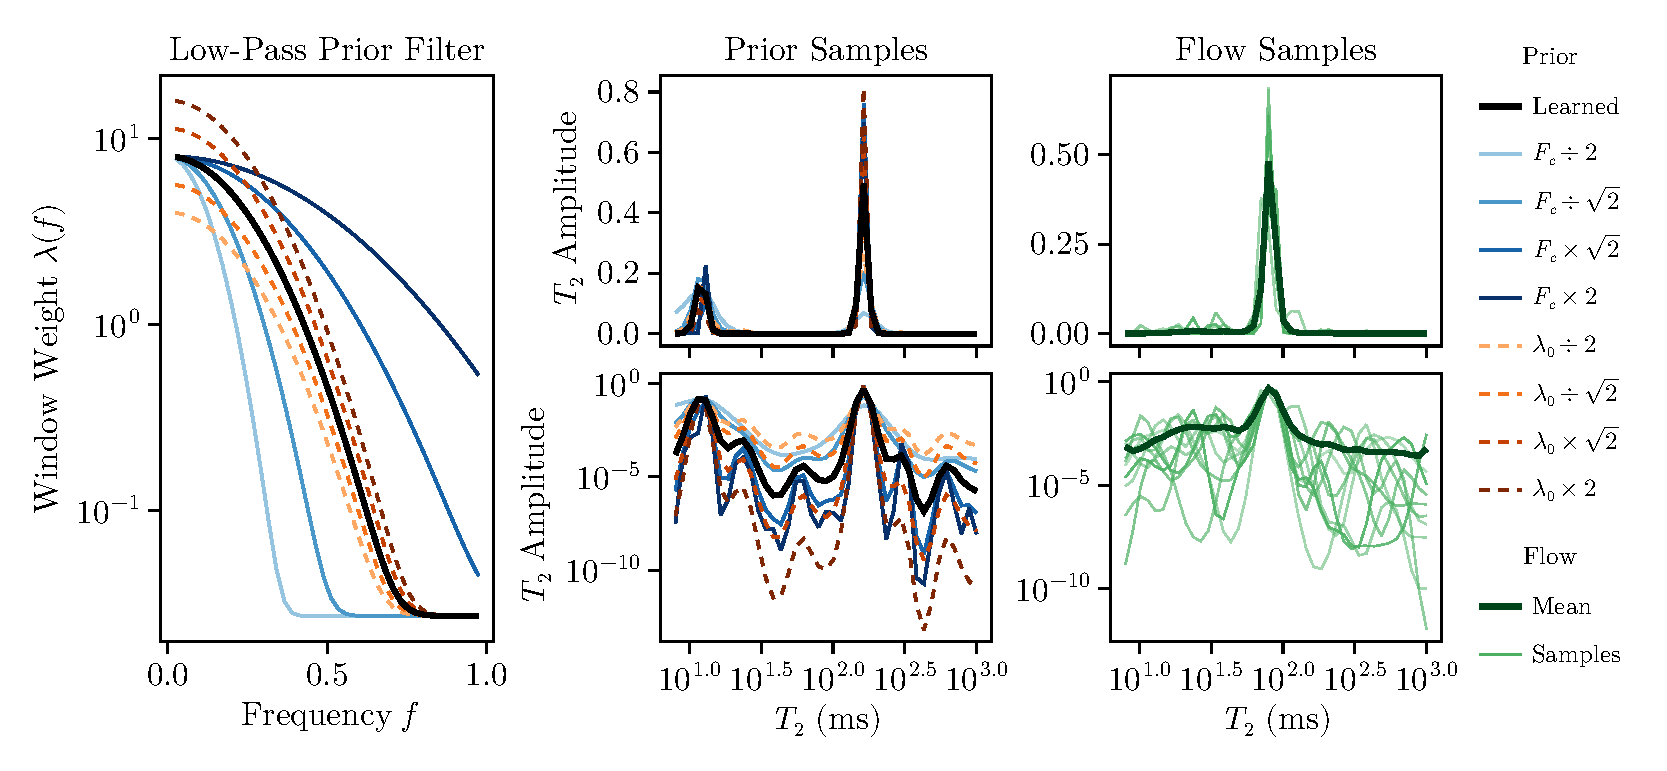
\includegraphics[width=\linewidth]{figures/prior_lowpass_filter.pdf}
    \caption{Learned low-pass window $\Lambda$ and its effect on $T_2$ spectra.
        The left panel shows the learned window weights $\lambda(f)$ alongside similar weights given by scaling either the cutoff $F_c$ or the amplitude $\lambda_0$ by factors $\tfrac{1}{2}$, $\tfrac{1}{\sqrt 2}$, $\sqrt 2$, and $2$.
        The middle panels show the effect of the differing parameters on the $T_2$ spectrum by pushing a fixed sample $\vv{u}$ through each window.
        The cutoff determines the overall smoothness while the amplitude controls the peak sharpness.
        The right panels show ten posterior samples from the trained flow for a representative voxel, shaded by importance weight, alongside the mean over \num{1000} samples.}
    \label{fig:prior_lowpass_filter}
\end{figure}

\section{Results}\label{sec:results}

\subsection{Data and Experimental Setup}\label{subsec:experimental_setup}

\paragraph*{Datasets.}
All images were acquired with a 32-channel head coil on a Philips \SI{3}{T} Ingenia Elition X scanner, subsequently upgraded to an MR 7700 (\cref{tab:scanner_protocol_inventory}).
The studies were approved by the University of British Columbia Clinical Research Ethics Board.
All participants provided written informed consent.
Images were split by subject into training ($\num{376}$ images, $156$ subjects; $298$ acquired before and $78$ after the upgrade), validation ($25$ images, $11$ subjects), and test ($94$ images, $34$ subjects) partitions, with no subject in more than one partition.
The partitions were separated before voxel extraction, and the validation partition was reserved for training monitoring.
Training and validation images, and the $21$ in-distribution (ID) test images from $11$ held-out subjects, were acquired using a 3D \gls*{MSE} sequence with $56$ echoes at \SI{7}{\ms} uniform echo spacing.
Acquired voxels are \SI[parse-numbers=false]{1.5 \times 2 \times 3}{\milli\meter\cubed} (\SI{3}{\milli\meter} slices with \SI{1.5}{\milli\meter} overlap), reconstructed at \SI[parse-numbers=false]{1 \times 1 \times 1.5}{\milli\meter\cubed}, except for $12$ images ($10$ training, $1$ validation, and $1$ ID test) acquired at \SI[parse-numbers=false]{2.5 \times 3 \times 3}{\milli\meter\cubed} and reconstructed at \SI{1.5}{\milli\meter} isotropic.
Quantitative in vivo evaluations used $\num{1000}$ masked voxels sampled uniformly from the ID test images.
For visualization, we also used an out-of-distribution (OOD) test image from a further held-out subject, acquired with $48$ echoes at \SI{8}{\ms} spacing and \SI{5}{\milli\meter} slices, reconstructed at \SI[parse-numbers=false]{0.96 \times 0.96 \times 2.5}{\milli\meter\cubed}, using a protocol excluded from training;
a representative axial slice was used for the in vivo maps.

\begin{table}[htbp]
    \centering
    \caption{Image counts by scanner and acquisition parameters for each partition.}
    \label{tab:scanner_protocol_inventory}
    \begin{tabular}{lrrrr}
    \toprule
                                      & Training & Validation & Test ID & Test shifted \\
    \midrule
    Total images                      & 376      & 25         & 21      & 73           \\
    \midrule
    \multicolumn{5}{l}{\textit{Scanner (Philips, 3 T)}}                                \\
    Ingenia Elition X                 & 298      & 20         & 14      & 73           \\
    MR 7700                           & 78       & 5          & 7       & 0            \\
    \midrule
    \multicolumn{5}{l}{\textit{Echoes / spacing (ms)}}                                 \\
    18 / 16                           & 0        & 0          & 0       & 7            \\
    24 / 12                           & 0        & 0          & 0       & 7            \\
    30 / 9.6                          & 0        & 0          & 0       & 7            \\
    36 / 8                            & 0        & 0          & 0       & 7            \\
    48 / 6                            & 0        & 0          & 0       & 6            \\
    48 / 6.05                         & 0        & 0          & 0       & 1            \\
    48 / 7.5                          & 0        & 0          & 0       & 1            \\
    48 / 8                            & 0        & 0          & 0       & 21           \\
    56 / 7                            & 376      & 25         & 21      & 16           \\
    \midrule
    \multicolumn{5}{l}{\textit{Repetition time (s)}}                                   \\
    1.07--1.14                        & 376      & 25         & 21      & 62           \\
    1.5                               & 0        & 0          & 0       & 6            \\
    2.0                               & 0        & 0          & 0       & 4            \\
    3.0                               & 0        & 0          & 0       & 1            \\
    \midrule
    \multicolumn{5}{l}{\textit{Slice thickness / spacing (mm)}}                        \\
    3 / 1.5                           & 376      & 25         & 21      & 15           \\
    3 / 1.8                           & 0        & 0          & 0       & 35           \\
    4 / 2                             & 0        & 0          & 0       & 3            \\
    5 / 2.5                           & 0        & 0          & 0       & 20           \\
    \midrule
    \multicolumn{5}{l}{\textit{Reconstructed voxel size (mm$^3$)}}                     \\
    0.936 $\times$ 0.936 $\times$ 1.5 & 0        & 0          & 0       & 1            \\
    0.938 $\times$ 0.938 $\times$ 1.5 & 0        & 0          & 0       & 2            \\
    0.938 $\times$ 0.938 $\times$ 2   & 0        & 0          & 0       & 3            \\
    0.958 $\times$ 0.958 $\times$ 2.5 & 0        & 0          & 0       & 19           \\
    1 $\times$ 1 $\times$ 1.5         & 366      & 24         & 20      & 12           \\
    1 $\times$ 1 $\times$ 2.5         & 0        & 0          & 0       & 1            \\
    1.5 $\times$ 1.5 $\times$ 1.5     & 10       & 1          & 1       & 0            \\
    1.797 $\times$ 1.797 $\times$ 1.8 & 0        & 0          & 0       & 35           \\
    \bottomrule
\end{tabular}

\end{table}

Brain masks were computed from the first echo with the Brain Extraction Tool (\gls*{BET})~\citep{smith_fast_2002} (fractional intensity threshold $0.6$, robust centre estimation) using the image voxel sizes;
for fields of view extending into the neck, the image was first reoriented to standard orientation and cropped with \texttt{robustfov}.
The training partition retained all masked voxels except for those with zero first-echo magnitude.
Signals are stored as integer echo amplitudes together with the signal bin width $\delta$ from the scan parameters;
signals $\signal$ and bin widths $\delta$ were normalized by the \gls*{DECAES} estimate of the initial signal magnitude, and the quantized Rician likelihood uses the resulting bin width $\delta$.
Echo trains were zero-padded to $n_{\TE} = 56$ echoes if needed.

The \gls*{EPG} basis matrix $\epgbases$ is constructed on a log-spaced $T_2$ grid using $n_{T_2} = 41$ bins over $[T_2^{\min}, T_2^{\max}]$.
This gives even Aitchison dimension $n_{T_2} - 1 = 40$, convenient for the coupling layers in the flow backbone.
At evaluation, $T_2^{\min} = \TE$ and $T_2^{\max} = T_1 = \SI{1}{s}$;
during training, $T_2^{\min}$, $T_2^{\max}$, $T_1$, and the flip angle are jittered by the augmentation pipeline of \cref{subsubsec:training_details}.

\paragraph*{Synthetic Evaluation Sets.}
We generated two synthetic test sets of $\num{1000}$ spectra each.
ID spectra were sampled from the learned prior $p(\bar{\distbn})$;
we refer to them as prior-sampled spectra.
We also generated OOD synthetic $T_2$ spectra with two Gaussian lobes in $\log T_2$.
The lobe centres were drawn uniformly from \SIrange{10}{25}{\ms} and \SIrange{50}{100}{\ms}, log-standard deviations from $[0.1,0.2]$, and short-$T_2$ mixture weights from $[0,0.25]$.
For both sets, signals were simulated using the same \gls*{EPG} forward model as in training and acquisition settings from the held-out ID test cohort, including voxelwise \gls*{DECAES} flip-angle estimates and normalized bin widths.
Ground-truth biomarkers were computed from the simulated $T_2$ spectra.
Quantized Rician noise was added at $\mathrm{SNR} \in \{\SI{30}{\decibel}, \SI{40}{\decibel}, \SI{50}{\decibel}\}$, with signal scale $s=1$ and $\sigma=10^{-\mathrm{SNR}_{\si{\decibel}}/20}$.
The lowest \gls*{SNR}, \SI{30}{\decibel}, is below typical in vivo levels.
All Bayesian methods and \gls*{DECAES} baselines were evaluated on the same $\num{1000}$ synthetic voxels and noise realizations for direct comparison.

\paragraph*{Baselines, References, and Metrics.}
\gls*{DECAES} was run using default settings with three regularization parameter selection methods (L-curve, \gls*{GCV}, and $\chi^2$)~\citep{doucette_decaes_2020}.

Posterior references use AdvancedHMC.jl~\citep{xu_advancedhmc_2020}, with $500$ \gls*{HMC} chains per voxel ($\num{1000}$ warmup and $\num{1000}$ retained draws) and $32$ \gls*{NUTS} chains ($\num{5000}$ warmup and $\num{5000}$ retained draws).
Both use the learned coordinates of the transformed posterior density.
Chains start from standard-normal draws and adapt their step size and diagonal mass to target acceptance $0.8$;
\gls*{HMC} uses $16$ leapfrog steps.
Identity-backbone \gls*{HMC} in \cref{subsec:preconditioning_ablation} instead investigates the unpreconditioned geometry.

\gls*{NUTS} evaluates densities, gradients, and sampler coordinates in double precision.
\gls*{HMC} evaluates log densities and gradients in single precision, while its internal state (positions, momenta, diagonal mass matrices, step sizes, and acceptance ratios) uses double precision.
The full \gls*{NUTS} reference covered $96$ held-out ID voxels ($\num{15360000}$ retained draws).
Its maximum rank-normalized split $\hat{R}$ was $1.0006$, and minimum spectrum-bin bulk and tail effective sample sizes were $\num{93878}$ and $\num{96951}$.
There were $46$ retained divergences across $28$ chains and $15$ voxels, and $27$ retained depth-limit transitions;
mean acceptance was $0.874$.
The three displayed \gls*{HMC} references had maximum $\hat{R}=1.0018$, minimum bulk/tail spectrum ESS $\num{297989}/\num{267155}$, and $0$ numerical-error iterations.
Across the $12$ displayed voxel/biomarker pairs, the maximum differences from the full \gls*{NUTS} means were $1.20$ combined Monte Carlo standard errors for \gls*{MALA} and $1.65$ for the displayed, thinned \gls*{HMC} estimator.
Monte Carlo errors use autocorrelation-adjusted \gls*{MALA} errors, full-chain \gls*{NUTS} diagnostics, and the independent retained-chain means for the thinned \gls*{HMC} estimator.

Removing all \gls*{NUTS} chains with retained divergences shifted the four biomarker means by at most $0.77$ full-reference Monte Carlo standard errors across the cohort, and $0.23$ for the displayed voxels.
This sensitivity analysis and the independent sampler comparisons do not exclude divergence-related bias.

\begin{table}[htbp]
    \centering
    \caption{Reference mixing diagnostics before pooling or thinning, across the voxels listed.
        The $\hat{R}$ maximum is over base coordinates, and bulk/tail effective-sample minima are over spectrum bins.
        Errors count retained \gls*{HMC} iterations with any numerical error and divergent \gls*{NUTS} transitions, respectively.}
    \label{tab:reference_diagnostics}
    \begin{tabular}{lrrrrrr}
    \toprule
    Reference & Voxels & Chains & Max. $\hat R$ & Min. bulk ESS & Min. tail ESS & Errors \\
    \midrule
    HMC       & 3      & 500    & 1.0018        & 297989        & 267155        & 0      \\
    NUTS      & 96     & 32     & 1.0006        & 93878         & 96951         & 46     \\
    \bottomrule
\end{tabular}

\end{table}

Accuracy on synthetic voxels is reported as the mean absolute error (\gls*{MAE}) of \gls*{MWF} in \si{\percent} and geometric mean $T_2$ in \si{\ms}, and as the Wasserstein-1 ($W_1$) distance between estimated and ground-truth normalized $T_2$ distributions over $\log T_2$.
Bayesian methods additionally report \SI{95}{\percent} credible-interval coverage of \gls*{MWF} and GM $T_2$, defined as the fraction of voxels for which the true value lies within the posterior \SI{95}{\percent} \gls*{CI}.

\subsection{Synthetic Data Evaluation}\label{subsec:synthetic_eval}

We first evaluated each method on the prior-sampled spectra described in~\cref{subsec:experimental_setup}, comparing \gls*{DECAES} against four Bayesian estimators:
direct sampling, importance-weighted (\gls*{IW}) sampling, Metropolis--Hastings (\gls*{MH}), and the Metropolis-adjusted Langevin algorithm (\gls*{MALA}).
Direct, \gls*{IW}, and \gls*{MH} estimates consumed $\num{1000}$ flow proposals per voxel, with \gls*{MALA} also requiring $\num{1000}$ gradient evaluations.
\gls*{DECAES} methods compute point estimates for comparison but report no analogous Bayesian coverage metrics.

\Cref{tab:synthetic_results} shows similar recovery errors across the Bayesian estimators, with lower mean errors than all \gls*{DECAES} methods on each reported recovery metric.
\Cref{fig:synthetic_voxel} illustrates this for a representative voxel, where the \gls*{MALA} posterior concentrates near the true spectrum, in contrast to the less accurate \gls*{DECAES} point estimates.

\begin{table}[htbp]
    \centering
    \caption{$T_2$ distribution recovery metrics over a batch of \num{1000} spectra drawn from the learned prior at \gls*{SNR} levels of $\SI{30}{\decibel}$, $\SI{40}{\decibel}$, and $\SI{50}{\decibel}$.
        \gls*{MWF} \gls*{MAE} in \si{\percent}, geometric mean $T_2$ \gls*{MAE}, and Wasserstein-1 ($W_1$) distances between estimated and ground-truth $T_2$ distributions are reported as mean $\pm$ standard deviation.
        \SI{95}{\percent} \gls*{CI} coverage of \gls*{MWF} and GM $T_2$ is reported for the Bayesian methods.
        Bold marks the lowest displayed mean error at each \gls*{SNR}.}
    \label{tab:synthetic_results}
    \begin{tabular}{clccccc}
  \toprule
                                               & Method  & \multicolumn{3}{c}{Mean errors} & \multicolumn{2}{c}{95\% coverage}                                                  \\
  \cmidrule(lr){3-5}\cmidrule(lr){6-7}
                                               &         & MWF (\%)                        & GM $T_2$ (ms)                     & $W_1$                    & MWF      & GM $T_2$ \\
  \midrule
  \multirow{7}{*}{\rotatebox{90}{SNR = 30 dB}} & L-Curve & $9.5 \pm 10.6$                  & $28.9 \pm 47.7$                   & $0.44 \pm 0.21$          & ---      & ---      \\
                                               & GCV     & $6.9 \pm 7.9$                   & $26.4 \pm 52.9$                   & $0.34 \pm 0.14$          & ---      & ---      \\
                                               & Chi2    & $6.8 \pm 7.9$                   & $26.5 \pm 52.8$                   & $0.34 \pm 0.14$          & ---      & ---      \\
                                               & Direct  & $3.8 \pm 5.8$                   & $6.1 \pm 10.4$                    & $\mathbf{0.18 \pm 0.11}$ & $93.6\%$ & $94.9\%$ \\
                                               & IW      & $\mathbf{3.7 \pm 5.7}$          & $\mathbf{5.8 \pm 9.6}$            & $\mathbf{0.18 \pm 0.11}$ & $93.7\%$ & $93.9\%$ \\
                                               & MH      & $\mathbf{3.7 \pm 5.6}$          & $\mathbf{5.8 \pm 9.6}$            & $\mathbf{0.18 \pm 0.11}$ & $93.1\%$ & $93.7\%$ \\
                                               & MALA    & $\mathbf{3.7 \pm 5.6}$          & $\mathbf{5.8 \pm 9.7}$            & $\mathbf{0.18 \pm 0.11}$ & $93.6\%$ & $94.2\%$ \\
  \midrule
  \multirow{7}{*}{\rotatebox{90}{SNR = 40 dB}} & L-Curve & $4.9 \pm 6.8$                   & $12.9 \pm 22.3$                   & $0.27 \pm 0.1$           & ---      & ---      \\
                                               & GCV     & $3.7 \pm 5.3$                   & $12.0 \pm 22.2$                   & $0.21 \pm 0.1$           & ---      & ---      \\
                                               & Chi2    & $3.6 \pm 5.0$                   & $12.1 \pm 22.7$                   & $0.2 \pm 0.1$            & ---      & ---      \\
                                               & Direct  & $\mathbf{2.1 \pm 3.5}$          & $\mathbf{3.2 \pm 5.9}$            & $\mathbf{0.11 \pm 0.08}$ & $95.1\%$ & $96.9\%$ \\
                                               & IW      & $\mathbf{2.1 \pm 3.5}$          & $\mathbf{3.2 \pm 5.8}$            & $\mathbf{0.11 \pm 0.08}$ & $94.7\%$ & $96.7\%$ \\
                                               & MH      & $\mathbf{2.1 \pm 3.5}$          & $\mathbf{3.2 \pm 5.8}$            & $\mathbf{0.11 \pm 0.08}$ & $94.9\%$ & $96.5\%$ \\
                                               & MALA    & $\mathbf{2.1 \pm 3.5}$          & $\mathbf{3.2 \pm 5.8}$            & $\mathbf{0.11 \pm 0.08}$ & $94.7\%$ & $96.4\%$ \\
  \midrule
  \multirow{7}{*}{\rotatebox{90}{SNR = 50 dB}} & L-Curve & $3.2 \pm 5.1$                   & $6.3 \pm 11.8$                    & $0.18 \pm 0.08$          & ---      & ---      \\
                                               & GCV     & $2.5 \pm 4.1$                   & $5.7 \pm 11.2$                    & $0.14 \pm 0.08$          & ---      & ---      \\
                                               & Chi2    & $2.2 \pm 3.7$                   & $5.7 \pm 11.1$                    & $0.13 \pm 0.08$          & ---      & ---      \\
                                               & Direct  & $\mathbf{1.4 \pm 2.6}$          & $2.2 \pm 4.1$                     & $\mathbf{0.08 \pm 0.06}$ & $95.0\%$ & $98.7\%$ \\
                                               & IW      & $\mathbf{1.4 \pm 2.5}$          & $\mathbf{2.1 \pm 4.0}$            & $\mathbf{0.08 \pm 0.06}$ & $95.2\%$ & $98.0\%$ \\
                                               & MH      & $\mathbf{1.4 \pm 2.5}$          & $\mathbf{2.1 \pm 4.0}$            & $\mathbf{0.08 \pm 0.06}$ & $95.0\%$ & $98.0\%$ \\
                                               & MALA    & $\mathbf{1.4 \pm 2.5}$          & $\mathbf{2.1 \pm 4.0}$            & $\mathbf{0.08 \pm 0.06}$ & $94.4\%$ & $97.3\%$ \\
  \bottomrule
\end{tabular}

\end{table}

\begin{figure}[ht]
    \centering
    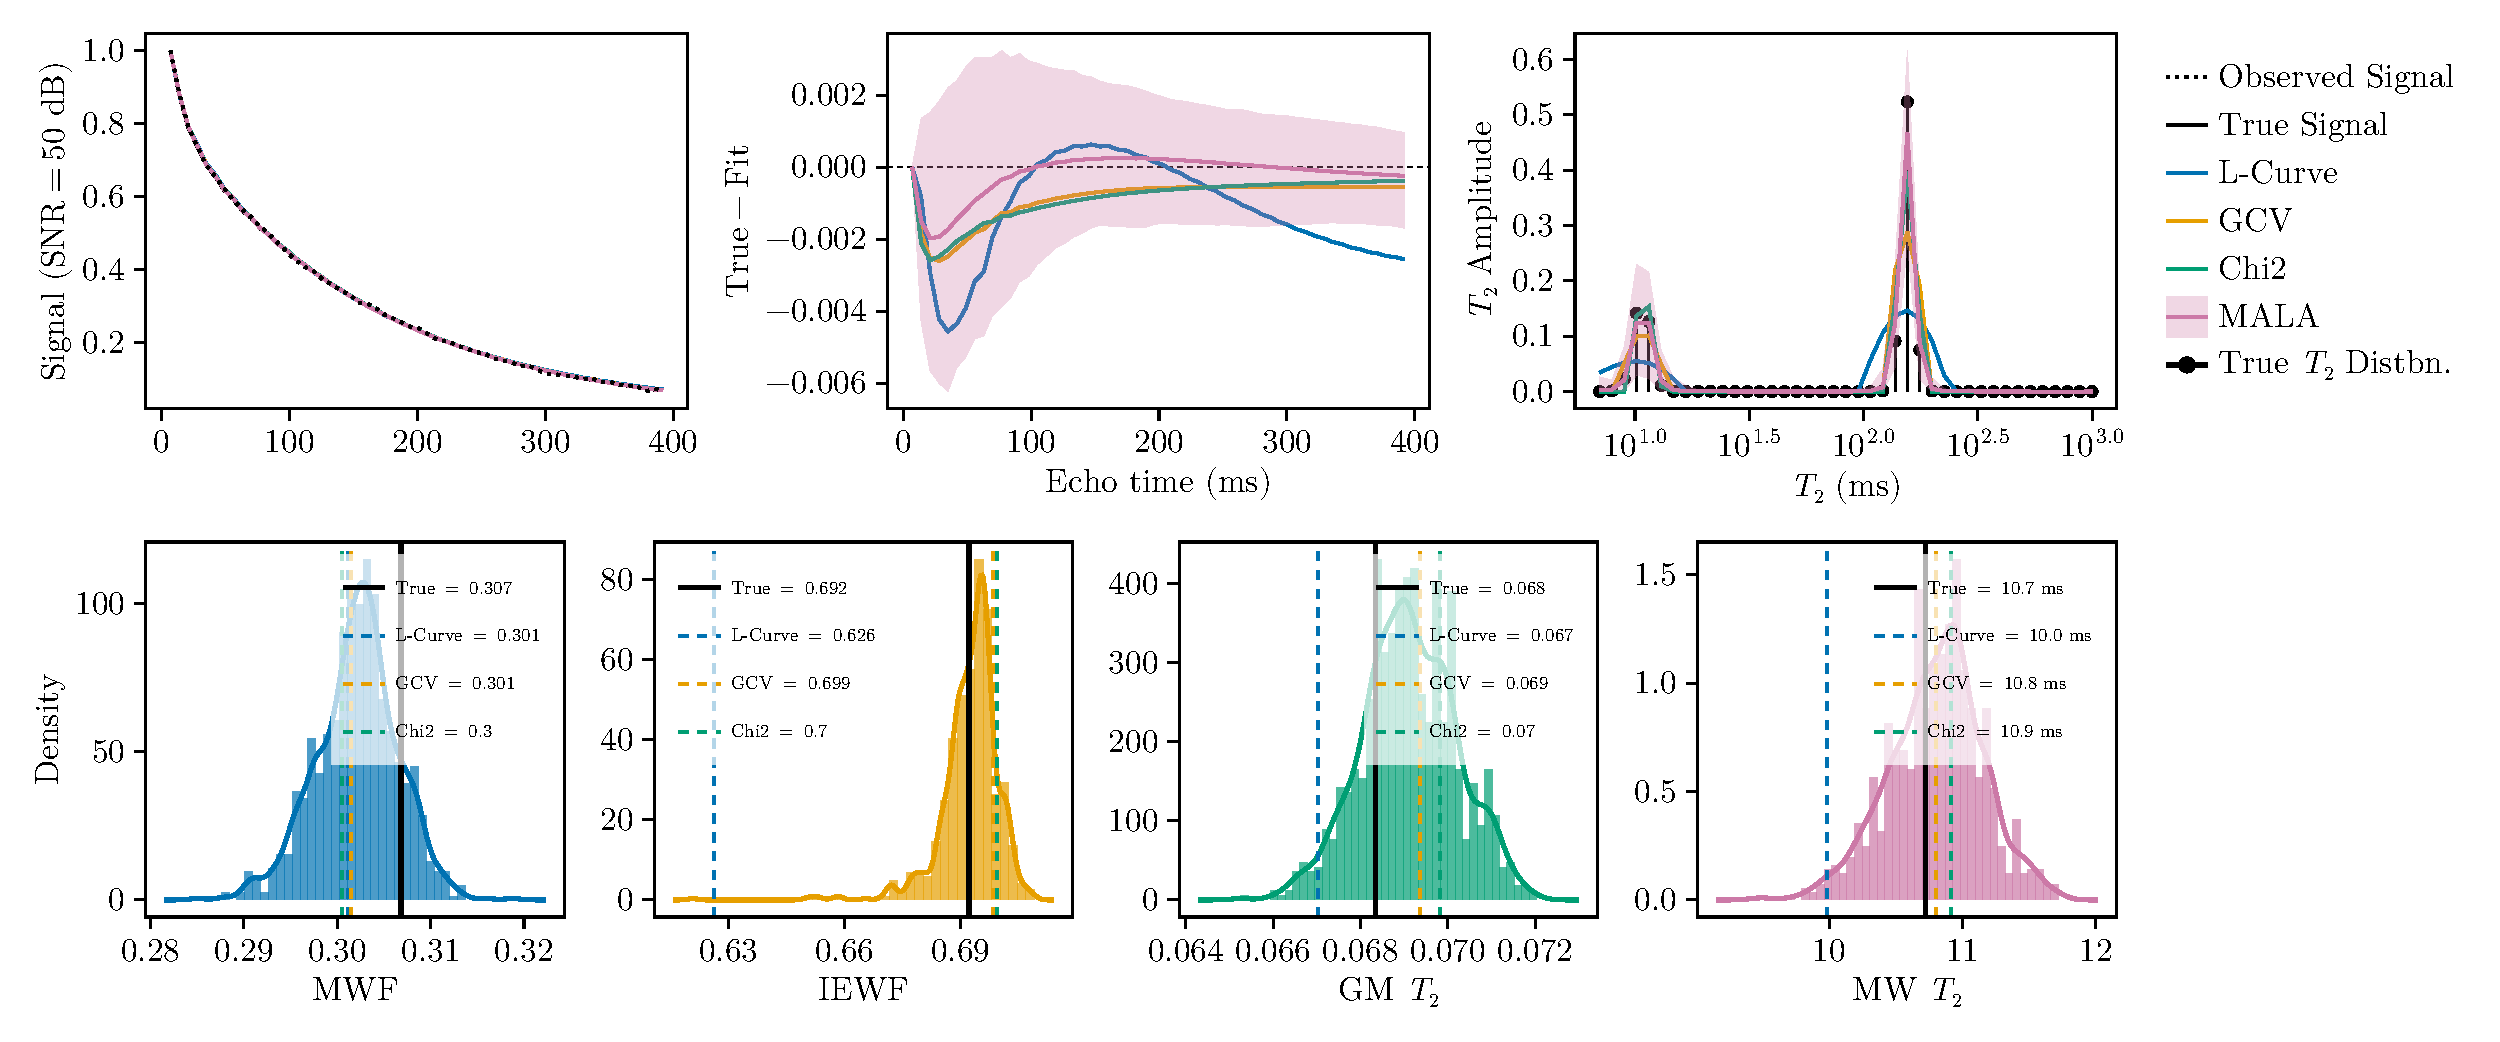
\includegraphics[width=\linewidth]{figures/synthetic_voxel.pdf}
    \caption{Inference comparison for the first prior-sampled spectrum at \SI{50}{\decibel}.
        Top row: multi-spin echo signal decay, signal fit residual, and recovered $T_2$ spectra, comparing the \gls*{DECAES} estimates with \gls*{MALA} posterior means and \SI{95}{\percent} credible bands.
        Bottom row: \gls*{MALA} posterior histograms for the \gls*{MWF}, \gls*{IEWF}, GM $T_2$, and MW $T_2$.}
    \label{fig:synthetic_voxel}
\end{figure}

\subsubsection{Posterior Calibration}\label{subsec:calibration}

A well-calibrated approximate posterior should produce observed coverage close to nominal coverage over a range of credible levels.
\Cref{fig:calibration} compares the coverages for \gls*{MALA}, \gls*{MH}, and \gls*{IW} at $\mathrm{SNR} = \SI{30}{\decibel}$, $\SI{40}{\decibel}$, and $\SI{50}{\decibel}$.
The three methods' calibration curves overlapped closely.
\gls*{MWF} coverage remained close to nominal;
GM $T_2$ intervals were conservative at \SIlist{40;50}{\decibel}.
At \SIlist{30;40;50}{\decibel}, nominal \SI{95}{\percent} \gls*{MWF} intervals covered \SIrange{93.1}{93.7}{\percent}, \SIrange{94.7}{95.1}{\percent}, and \SIrange{94.4}{95.2}{\percent} of true values across the four Bayesian estimators (\cref{tab:synthetic_results}).
GM $T_2$ coverage was \SIrange{93.7}{94.9}{\percent}, \SIrange{96.4}{96.9}{\percent}, and \SIrange{97.3}{98.7}{\percent}, respectively.
MW $T_2$ coverage was \SIrange{92.6}{94.9}{\percent} across the tested \gls*{SNR}s.

\begin{figure}[ht]
    \centering
    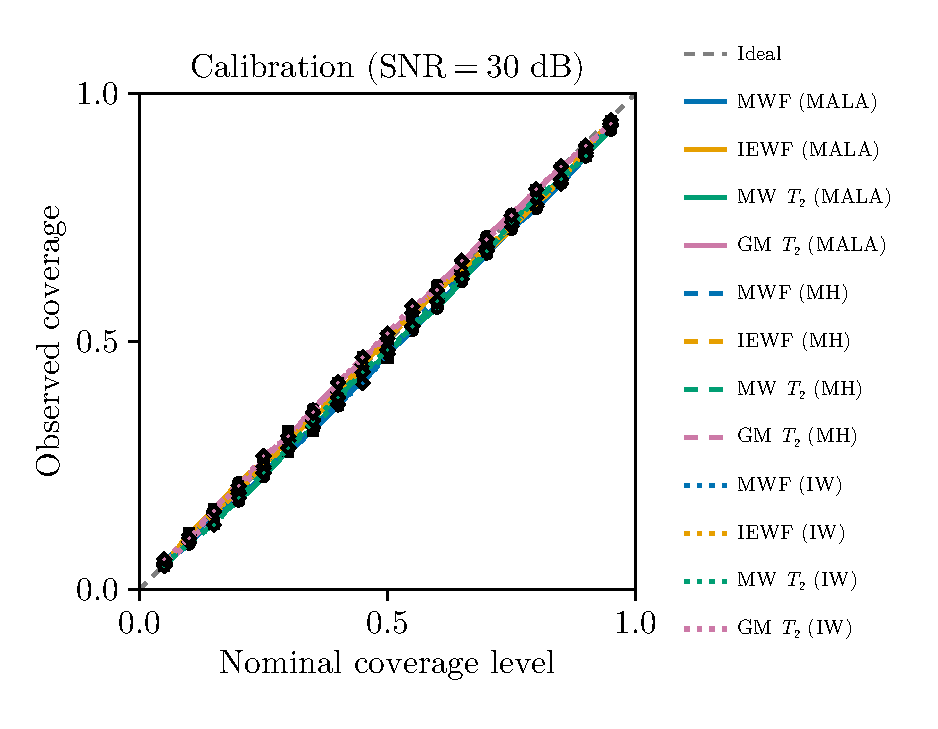
\includegraphics[width=0.32\linewidth]{figures/calibration_30dB.pdf}\hfill
    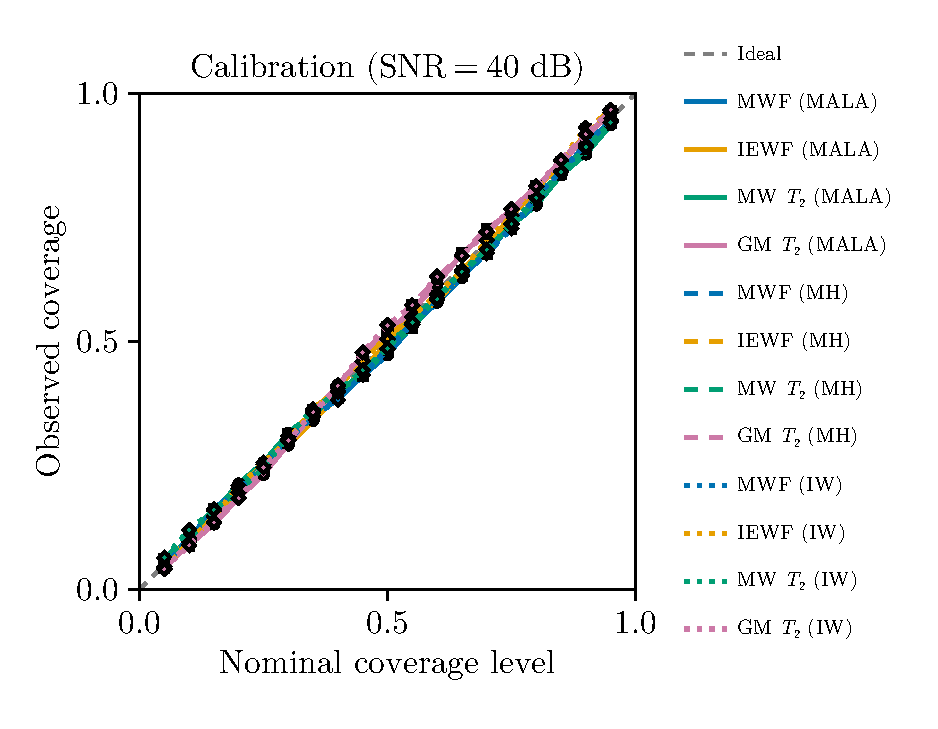
\includegraphics[width=0.32\linewidth]{figures/calibration_40dB.pdf}\hfill
    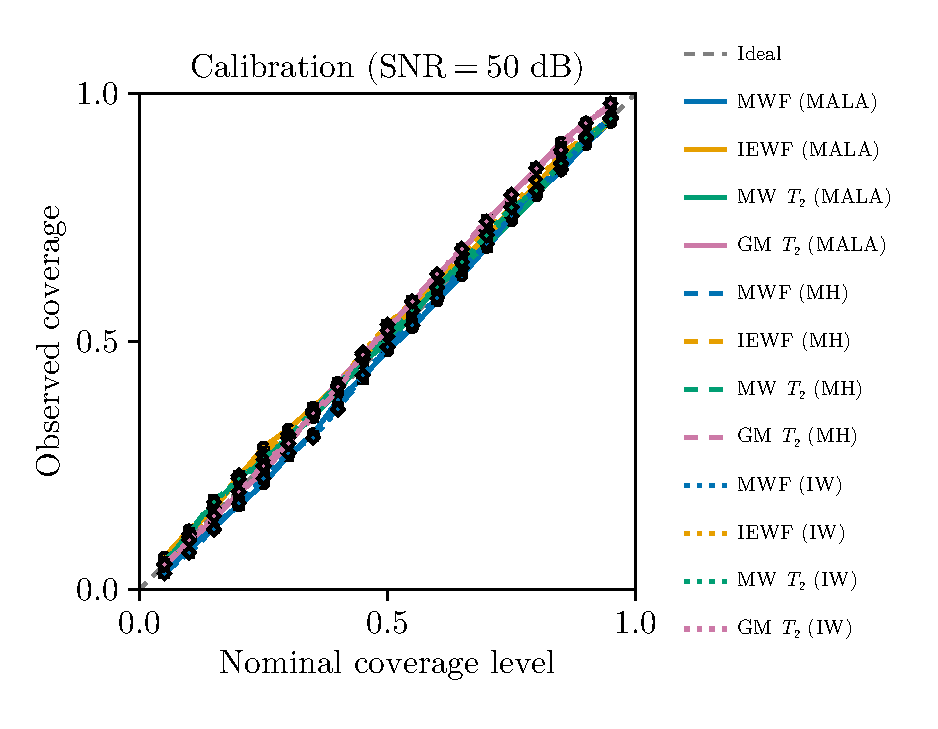
\includegraphics[width=0.32\linewidth]{figures/calibration.pdf}
    \caption{Calibration plots for \gls*{MALA}, \gls*{MH}, and \gls*{IW} on synthetic data with $\mathrm{SNR} = \SI{30}{\decibel}$ (left), $\SI{40}{\decibel}$ (middle), and $\SI{50}{\decibel}$ (right).
        Observed posterior coverage is compared with nominal credible levels for each biomarker;
        perfect calibration lies along $y = x$.}
    \label{fig:calibration}
\end{figure}

\subsubsection{Bimodal Synthetic Spectra}\label{subsec:bimodal_calibration}

We repeated the recovery evaluation using the OOD bimodal spectra defined in \cref{subsec:experimental_setup}, retaining the acquisition settings, noise levels, and inference budgets (\cref{tab:synthetic_bimodal_results,fig:synthetic_prior_comparison}).
\gls*{MWF} coverage was \SIrange{86.7}{88.9}{\percent}, \SIrange{91.7}{92.4}{\percent}, and \SIrange{98.2}{98.5}{\percent} at \SIlist{30;40;50}{\decibel}, respectively, showing sensitivity to the spectrum distribution.
The prior-sampled spectra span a broader range of compartment fractions and should not be interpreted as the empirical distribution of brain spectra.
For the prior-sampled benchmark, median importance-weight $\mathrm{ESS}/S$ was $0.78$, $0.85$, and $0.76$;
no voxel had $\widehat{k}>0.7$ at any \gls*{SNR}, with maximum $\widehat{k} = 0.69$.
All voxels were retained.

\begin{table}[htbp]
    \centering
    \caption{$T_2$ recovery for $\num{1000}$ synthetic bimodal $T_2$ spectra, using the acquisition settings and inference budgets of \cref{tab:synthetic_results}.
        Errors are reported as mean $\pm$ standard deviation;
        \SI{95}{\percent} \gls*{CI} coverage is reported for the Bayesian methods.
        Bold marks the lowest displayed mean error at each \gls*{SNR}.}
    \label{tab:synthetic_bimodal_results}
    \begin{tabular}{clccccc}
  \toprule
                                               & Method  & \multicolumn{3}{c}{Mean errors} & \multicolumn{2}{c}{95\% coverage}                                                  \\
  \cmidrule(lr){3-5}\cmidrule(lr){6-7}
                                               &         & MWF (\%)                        & GM $T_2$ (ms)                     & $W_1$                    & MWF      & GM $T_2$ \\
  \midrule
  \multirow{7}{*}{\rotatebox{90}{SNR = 30 dB}} & L-Curve & $10.2 \pm 8.1$                  & $5.1 \pm 4.0$                     & $0.36 \pm 0.06$          & ---      & ---      \\
                                               & GCV     & $7.4 \pm 5.6$                   & $6.4 \pm 5.4$                     & $0.33 \pm 0.08$          & ---      & ---      \\
                                               & Chi2    & $7.5 \pm 5.6$                   & $6.7 \pm 5.7$                     & $0.33 \pm 0.09$          & ---      & ---      \\
                                               & Direct  & $6.0 \pm 4.7$                   & $2.3 \pm 1.8$                     & $0.18 \pm 0.08$          & $86.7\%$ & $90.6\%$ \\
                                               & IW      & $\mathbf{5.6 \pm 4.5}$          & $\mathbf{2.1 \pm 1.6}$            & $\mathbf{0.17 \pm 0.08}$ & $88.9\%$ & $91.1\%$ \\
                                               & MH      & $\mathbf{5.6 \pm 4.5}$          & $\mathbf{2.1 \pm 1.6}$            & $\mathbf{0.17 \pm 0.08}$ & $88.4\%$ & $91.1\%$ \\
                                               & MALA    & $\mathbf{5.6 \pm 4.5}$          & $\mathbf{2.1 \pm 1.6}$            & $\mathbf{0.17 \pm 0.08}$ & $88.0\%$ & $90.5\%$ \\
  \midrule
  \multirow{7}{*}{\rotatebox{90}{SNR = 40 dB}} & L-Curve & $5.1 \pm 3.5$                   & $2.5 \pm 2.2$                     & $0.2 \pm 0.04$           & ---      & ---      \\
                                               & GCV     & $4.6 \pm 3.6$                   & $3.5 \pm 3.0$                     & $0.17 \pm 0.06$          & ---      & ---      \\
                                               & Chi2    & $4.4 \pm 3.6$                   & $3.6 \pm 3.1$                     & $0.16 \pm 0.06$          & ---      & ---      \\
                                               & Direct  & $\mathbf{3.0 \pm 2.8}$          & $\mathbf{0.8 \pm 0.6}$            & $\mathbf{0.09 \pm 0.03}$ & $92.3\%$ & $97.2\%$ \\
                                               & IW      & $\mathbf{3.0 \pm 2.8}$          & $\mathbf{0.8 \pm 0.7}$            & $\mathbf{0.09 \pm 0.03}$ & $92.4\%$ & $96.9\%$ \\
                                               & MH      & $\mathbf{3.0 \pm 2.8}$          & $\mathbf{0.8 \pm 0.7}$            & $\mathbf{0.09 \pm 0.03}$ & $92.4\%$ & $96.6\%$ \\
                                               & MALA    & $\mathbf{3.0 \pm 2.8}$          & $\mathbf{0.8 \pm 0.7}$            & $\mathbf{0.09 \pm 0.03}$ & $91.7\%$ & $96.1\%$ \\
  \midrule
  \multirow{7}{*}{\rotatebox{90}{SNR = 50 dB}} & L-Curve & $3.2 \pm 2.3$                   & $1.8 \pm 1.5$                     & $0.12 \pm 0.04$          & ---      & ---      \\
                                               & GCV     & $2.4 \pm 2.2$                   & $1.7 \pm 1.6$                     & $0.08 \pm 0.04$          & ---      & ---      \\
                                               & Chi2    & $2.2 \pm 2.0$                   & $1.7 \pm 1.6$                     & $0.08 \pm 0.04$          & ---      & ---      \\
                                               & Direct  & $\mathbf{1.3 \pm 1.2}$          & $\mathbf{0.4 \pm 0.3}$            & $\mathbf{0.06 \pm 0.02}$ & $98.3\%$ & $99.7\%$ \\
                                               & IW      & $\mathbf{1.3 \pm 1.2}$          & $\mathbf{0.4 \pm 0.3}$            & $\mathbf{0.06 \pm 0.02}$ & $98.5\%$ & $99.7\%$ \\
                                               & MH      & $\mathbf{1.3 \pm 1.2}$          & $\mathbf{0.4 \pm 0.3}$            & $\mathbf{0.06 \pm 0.02}$ & $98.3\%$ & $99.6\%$ \\
                                               & MALA    & $\mathbf{1.3 \pm 1.2}$          & $\mathbf{0.4 \pm 0.3}$            & $\mathbf{0.06 \pm 0.02}$ & $98.2\%$ & $99.6\%$ \\
  \bottomrule
\end{tabular}

\end{table}

\begin{figure}[htbp]
    \centering
    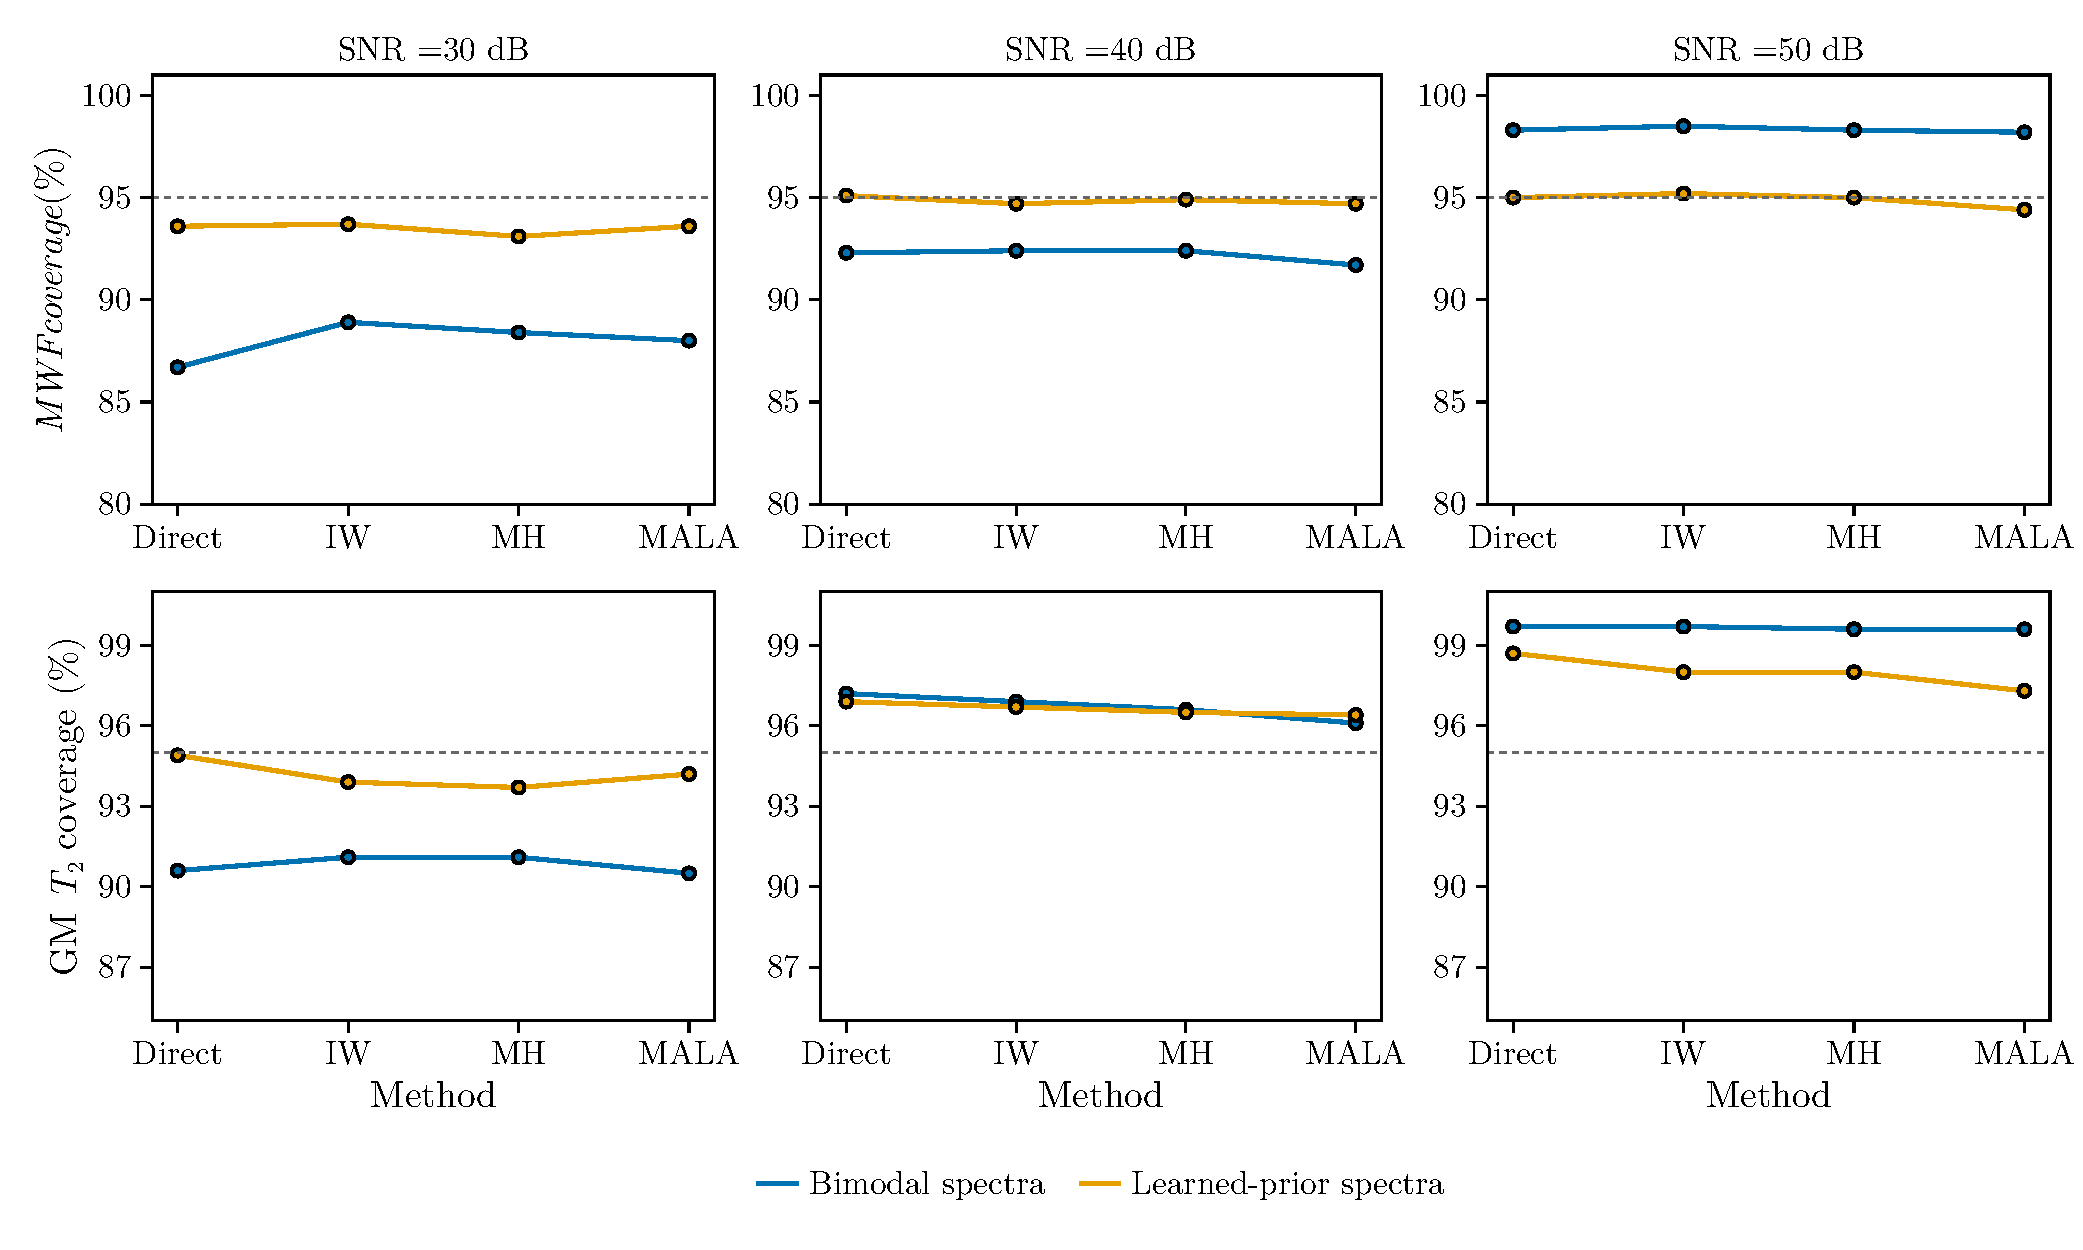
\includegraphics[width=\linewidth]{figures/synthetic_prior_comparison.pdf}
    \caption{Observed \SI{95}{\percent} interval coverage for synthetic bimodal and learned-prior spectra.
        Columns correspond to \SIlist{30;40;50}{\decibel};
        rows show \gls*{MWF} and GM $T_2$.
        The dashed line marks nominal coverage.}
    \label{fig:synthetic_prior_comparison}
\end{figure}

\subsection{In Vivo Evaluation}\label{subsec:invivo_eval}

In vivo multi-spin echo brain data were processed using \gls*{DECAES} and two Bayesian sampling methods, \gls*{MALA} and \gls*{MH}.
\Cref{fig:invivo_comparison} shows \gls*{MWF} and geometric mean $T_2$ maps for a single axial brain slice.
The Bayesian posterior means produce \gls*{MWF} maps that are smoother and more spatially uniform than \gls*{DECAES}, with sharper white-matter and grey-matter contrast and boundaries.
The $\text{\gls*{DECAES}}-\text{\gls*{MH}}$ difference maps show coherent spatial structure rather than unstructured noise, suggesting nontrivial differences in the recovered spectra.
The posterior \gls*{CI} half-width maps illustrate voxelwise estimated uncertainty, generally scaling in proportion to the magnitude of the estimated parameter.
For the full volume (\num{645006} masked voxels), sampling required approximately \SI{0.3}{\second}/sample for \gls*{IW}/\gls*{MH}/\gls*{RWM} and \SI{0.9}{\second}/sample for \gls*{MALA} on one RTX 8000 GPU.

\Cref{fig:xdist_comparison} shows mean $T_2$ spectra for three voxel cluster partitions for a held-out test image slice, roughly corresponding to white matter, grey matter, and \gls*{CSF}, for each \gls*{DECAES} method as well as \gls*{MH}.
Voxels were grouped into one of three clusters according to which water fraction -- myelin, intra-/extracellular, or cerebrospinal-fluid -- is most elevated relative to the slice average;
the resulting clusters are shown in the rightmost panel.
The \gls*{MH} spectra resolve more cleanly separated $T_2$ peaks than any \gls*{DECAES} method, whose intra-/extracellular peak is broader -- plausibly an artifact of over-regularization in the \gls*{NNLS} solver -- and whose myelin-water peak is smaller and more clustered toward the $T_2^{\min}$ boundary.

\begin{figure}[ht]
    \centering
    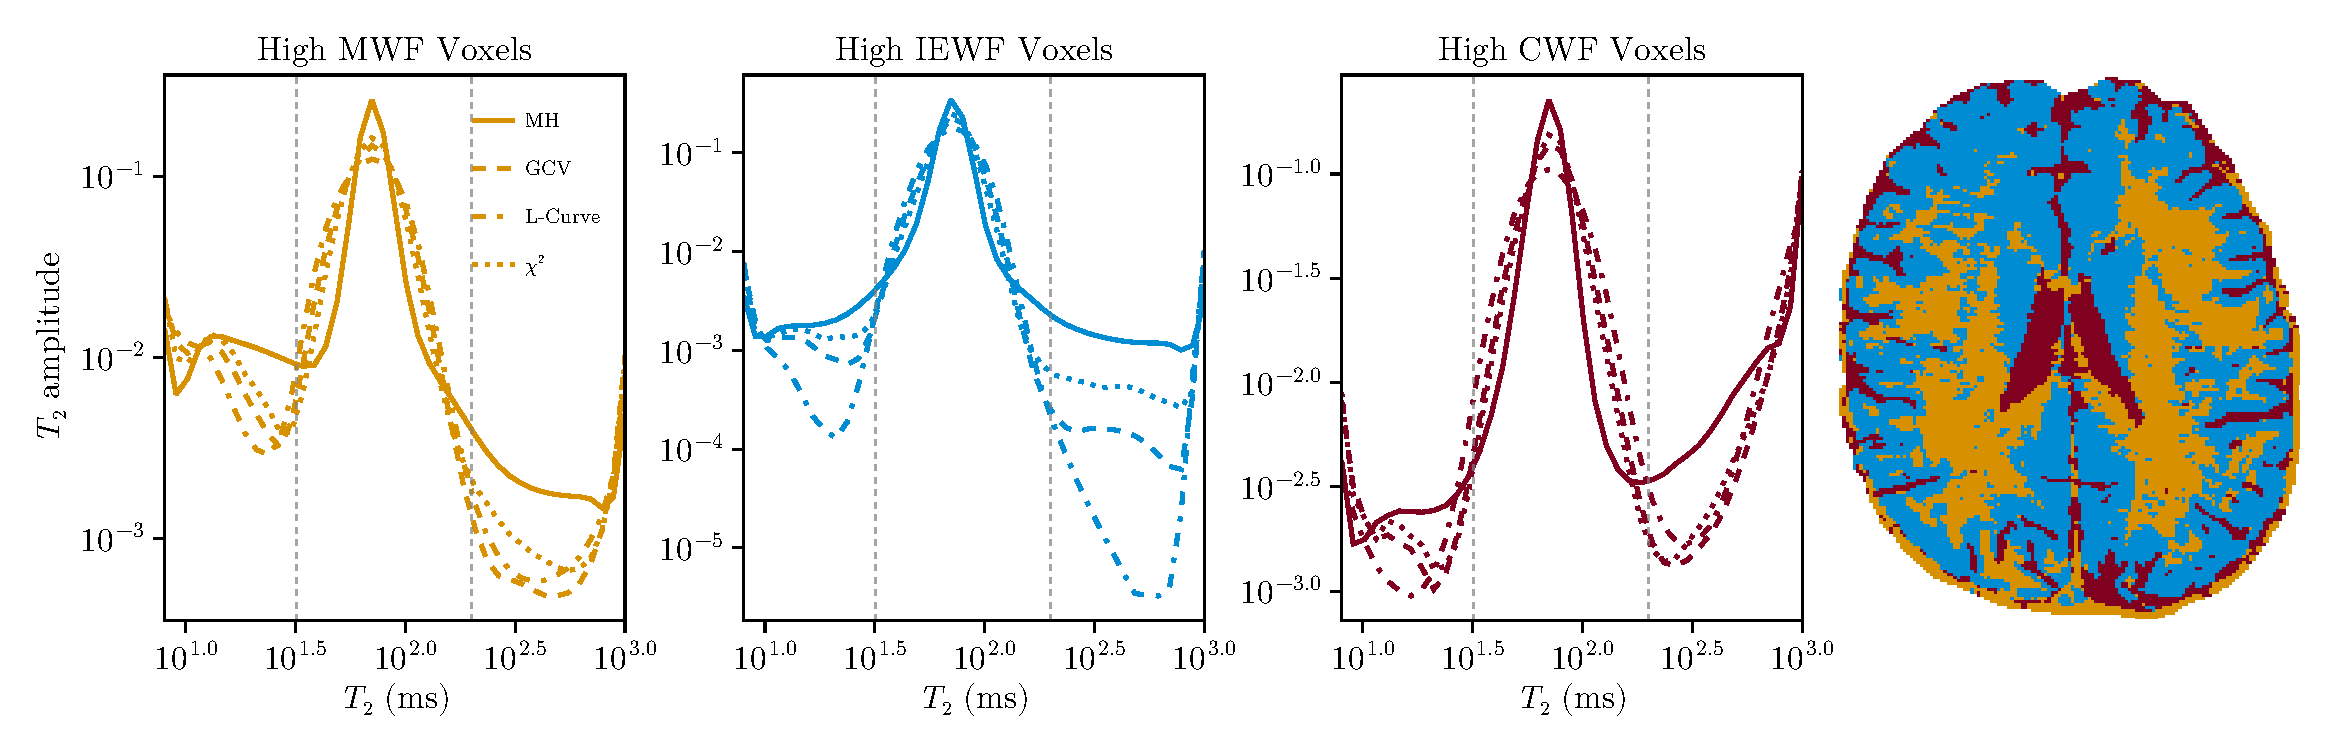
\includegraphics[width=\linewidth]{figures/xdist_comparison.pdf}
    \caption{Cluster-mean $T_2$ spectra on a held-out test image slice, with voxels partitioned by dominant water fraction relative to the slice mean.
        First three panels: \gls*{MH} posterior mean overlaid on the \gls*{DECAES} L-curve, \gls*{GCV}, and $\chi^2$ estimates.
        Rightmost panel: voxel cluster assignments.}
    \label{fig:xdist_comparison}
\end{figure}

\Cref{fig:posterior_samples} compares learned-coordinate \gls*{MALA} with the pooled \gls*{HMC} and \gls*{NUTS} references for three in vivo voxels with high myelin, intra-/extracellular, or cerebrospinal-fluid fractions.
The spectra and biomarker histograms agree closely, supporting the untuned \gls*{MALA} estimates and the consistency of the two references.

\begin{figure}[ht]
    \centering
    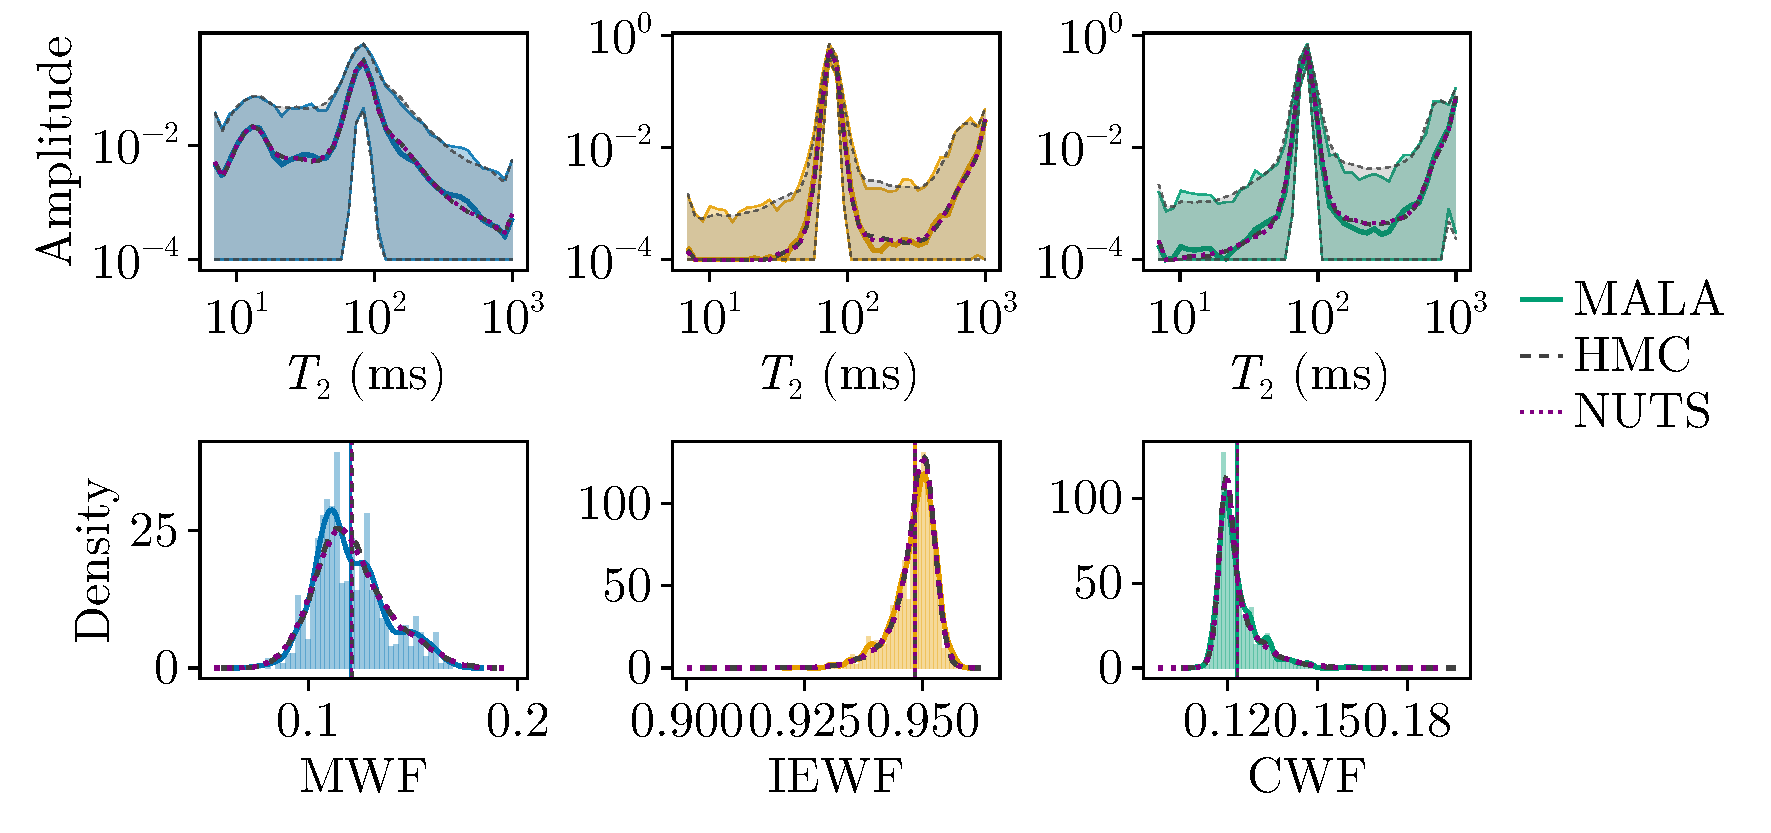
\includegraphics[width=\linewidth]{figures/posterior_samples.pdf}
    \caption{Posterior distributions for three representative in vivo voxels, comparing posterior samples using \gls*{MALA} (without warmup or step size tuning), \gls*{HMC}, and \gls*{NUTS}.
        Each column corresponds to a single voxel.
        Top row: $T_2$ spectra posterior mean and \SI{95}{\percent} credible band.
        Bottom row: biomarker empirical posterior histograms with overlaid kernel density estimates and vertical lines indicating posterior means.}
    \label{fig:posterior_samples}
\end{figure}

\subsubsection{Posterior Quality and \texorpdfstring{\gls*{MCMC}}{MCMC} Diagnostics}\label{subsec:diagnostics}

The Pareto-smoothed importance sampling (\gls*{PSIS}) diagnostic $\hat{k}$ is used to flag unreliable posterior approximations by identifying voxels with heavy-tailed importance weights, characterized by $\hat{k} > 0.7$~\citep{vehtari_pareto_2022,yao_yes_2018}, which lead to high-variance estimators.
\Cref{fig:psis_diagnostic} shows that $948$ of the $\num{1000}$ ID test voxels satisfied $\hat{k}<0.5$, and $3$ exceeded $0.7$.
The mean normalized importance effective sample size was $\mathrm{ESS}/S=0.826$ for $S = \num{1000}$ proposals, with $939$ voxels satisfying $\mathrm{ESS}/S>0.7$.
\begin{figure}[ht]
    \centering
    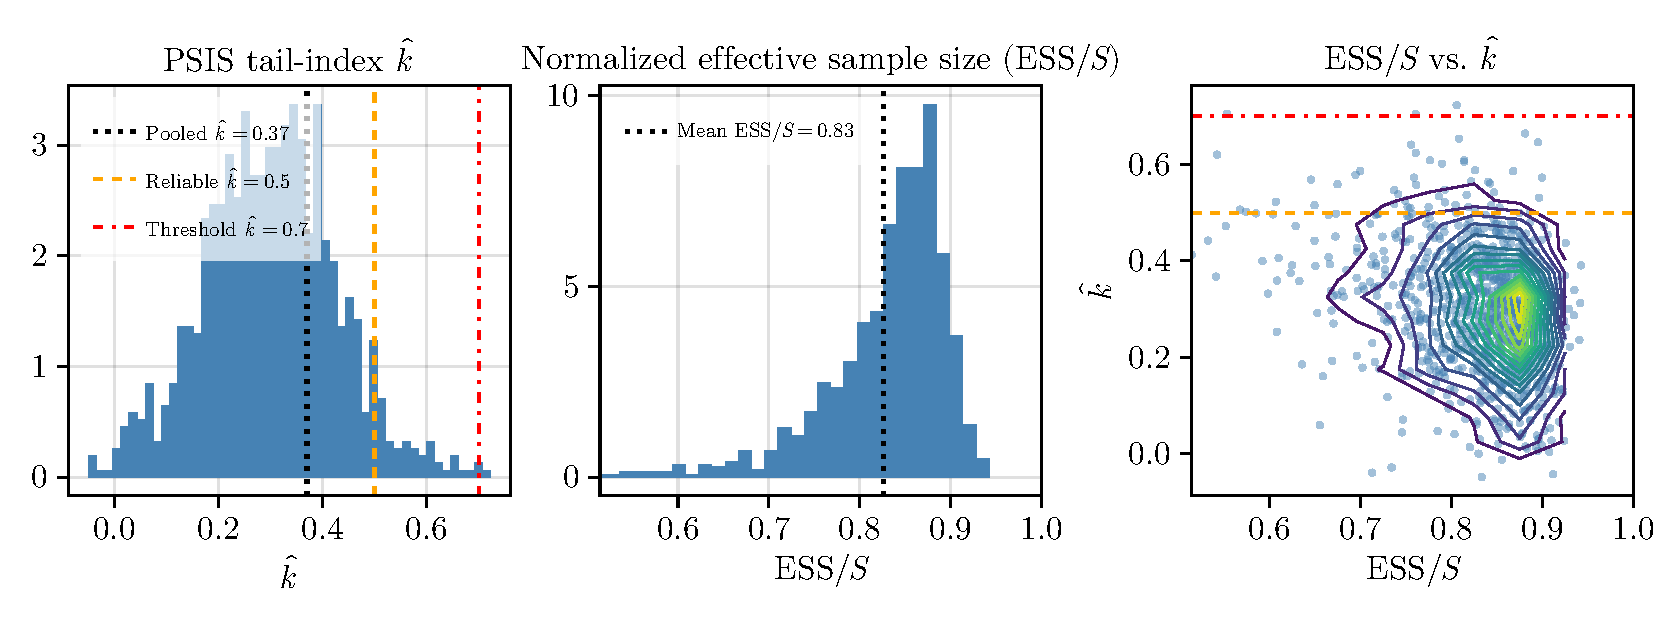
\includegraphics[width=\linewidth]{figures/psis_diagnostic.pdf}
    \caption{\gls*{PSIS} diagnostic $\hat{k}$ and normalized effective sample size $\mathrm{ESS}/S$ for the variational posterior.
        Both quantities are computed from self-normalized importance weights.
        The panels show the $\hat{k}$ and $\mathrm{ESS}/S$ marginal and joint distributions over the $\num{1000}$ ID test voxels.}
    \label{fig:psis_diagnostic}
\end{figure}

\Cref{fig:mcmc_diagnostics} shows sampling convergence diagnostics for \gls*{MALA} and \gls*{MH} on the ID test cohort.
The \gls*{MALA} acceptance distribution concentrated around a mean of $0.547$, close to the asymptotically optimal value $0.574$~\citep{roberts_optimal_1998}, while independent-proposal \gls*{MH} attained a mean acceptance of $0.785$.
For \gls*{MALA}, we report the integrated autocorrelation time $\tau^{\mathrm{int}}$ of each biomarker sampling chain, as estimated by the self-consistent windowing method~\citep{sokal_monte_1997}.
For independent-proposal \gls*{MH}, an autocorrelation time $\tau^{\mathrm{int}}_{\mathrm{Acc.}}$ may be estimated directly from the accept-reject sequence of the chain~\citep{albergo_flow-based_2019}.
The median \gls*{MWF} autocorrelation time was $0.84$ steps for \gls*{MH} and $3.22$ steps for \gls*{MALA};
the median \gls*{MH} acceptance-sequence estimate was $\tau^{\mathrm{int}}_{\mathrm{Acc.}} = 0.82$ steps.

\begin{figure}[ht]
    \centering
    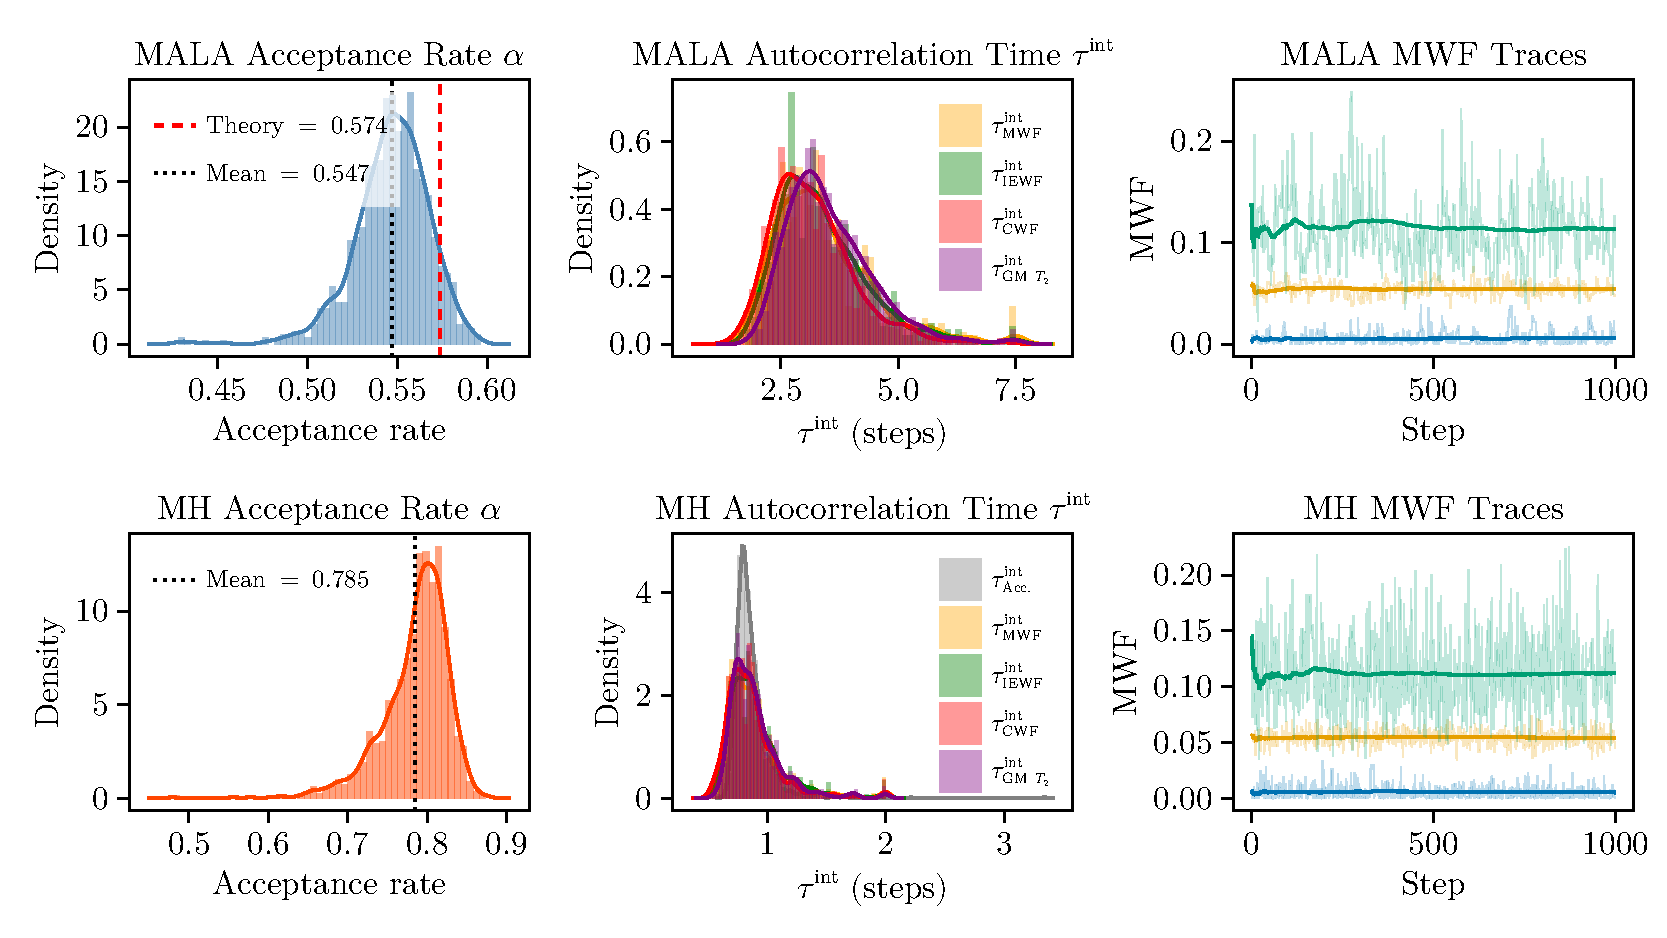
\includegraphics[width=\linewidth]{figures/mcmc_diagnostics.pdf}
    \caption{\gls*{MCMC} convergence diagnostics over the ID test voxels.
        Rows show \gls*{MALA} (top) and independent-proposal \gls*{MH} (bottom).
        The first column shows the acceptance rate;
        for \gls*{MALA}, the mean is close to the asymptotically optimal rate $0.574$.
        The second column shows integrated autocorrelation times $\tau^{\mathrm{int}}$;
        for \gls*{MALA}, $\tau^{\mathrm{int}}$ is estimated only from the biomarker chains, but for \gls*{MH}, it can additionally be estimated from the acceptance sequence.
        The third column shows \gls*{MWF} chain traces with overlaid cumulative means.}
    \label{fig:mcmc_diagnostics}
\end{figure}

\subsection{Preconditioning Ablation}\label{subsec:preconditioning_ablation}

To investigate the benefit of preconditioning by the learned flow, we compared \gls*{MALA} in the flow-transformed base coordinates $\vv{u}$ against both \gls*{MALA} and \gls*{HMC} with an identity-flow backbone, replacing the deep conditional flow $\varphi_{\vv{\xi}}(\cdot; \signal)$ with the identity map.
This retains the low-pass window, inverse \gls*{ILR}, and conditional nuisance transformation, sampling the pre-window coordinates $\vv{\xi} = \varphi_{\vv{\xi}}(\vv{u}_{\bar{\distbn}}; \signal)$ directly.
This ablation used the OOD bimodal spectra of \cref{subsec:experimental_setup} at \SI{50}{\decibel}.
In \cref{fig:flow_geometry}, learned-backbone \gls*{MALA} used the theoretical step size without warmup;
identity-backbone \gls*{MALA} adapted its step size per voxel over $\num{4000}$ warmup iterations, targeting an acceptance ratio of $0.574$;
identity-backbone \gls*{HMC} used eight chains per voxel with $\num{1000}$ warmup iterations and $16$ leapfrog steps per draw.
Each method retained $\num{1000}$ draws per chain.

\Cref{fig:flow_geometry} shows a roughly twentyfold reduction in median mean-coordinate autocorrelation time.
Interpolating between the same approximate-posterior $T_2$ spectra, we see that extremely low-density regions in pre-window $\vv{\xi}$ coordinates must be traversed.
This is in stark contrast to interpolation in learned $\vv{u}$ coordinates, wherein one remains in high posterior density regions throughout the entire interpolation path.
We further see that the learned-backbone chain explores the displayed marginal posterior more broadly, with the identity-backbone chains instead becoming stuck in confined regions, unable to escape despite having access to posterior gradient information;
even \gls*{HMC}, with an adapted diagonal metric, fails to explore the whole marginal space.

\begin{figure}[ht]
    \centering
    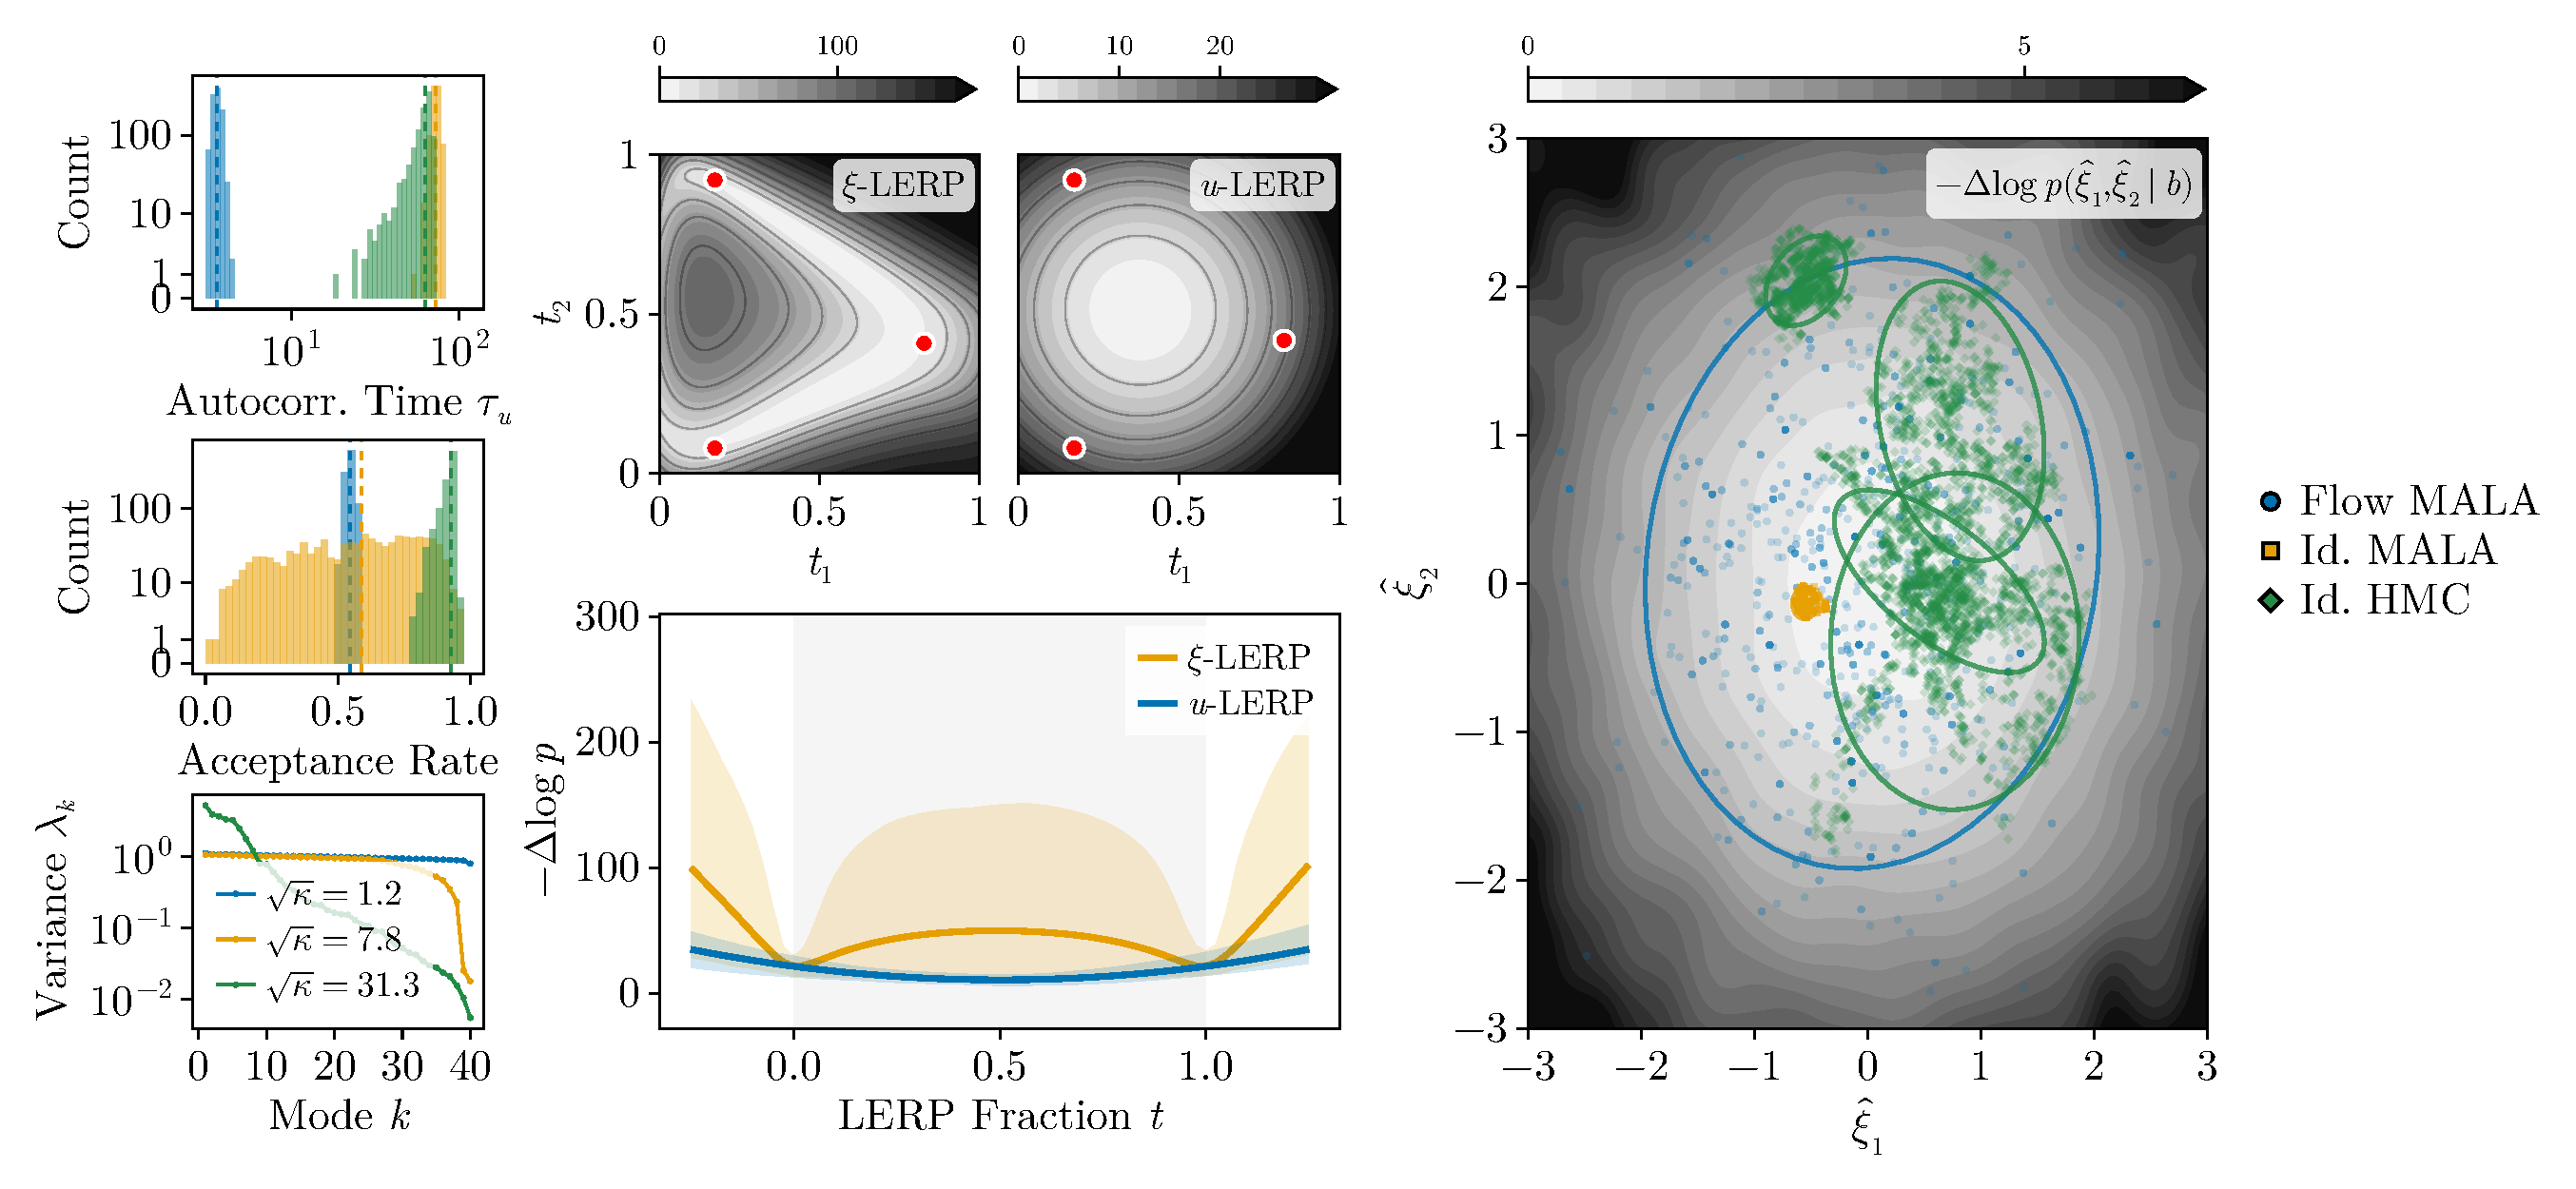
\includegraphics[width=\linewidth]{figures/flow_geometry.pdf}
    \caption{Illustration of the effect of the learned preconditioning on the posterior geometry and on sampling.
        Three sampling procedures are shown:
        \gls*{MALA} under the learned flow, and both \gls*{MALA} and \gls*{HMC} where the learned flow backbone $\varphi_{\vv{\xi}}$ is replaced with the identity transform.
        The left column shows the across-voxel diagnostics for batches of sample sequences $\{\vv{u}_t\}$:
        histograms of the mean autocorrelation time $\tau_u$ and the acceptance rates, with their medians marked;
        and the eigenvalue spectrum $\lambda_k$ of the importance-weighted proposal covariances in the learned and pre-window coordinates and the pooled \gls*{HMC} sample covariance in pre-window coordinates, with covariance aspect ratio $\sqrt{\kappa}$ annotated.
        The middle column shows negative-log-posterior slices through three i.i.d.\ standard-normal $u$ points and their pre-window \gls*{ILR} images $\vv{\xi}$ (top), and straight-chord profiles with weight $t$, averaged over $100$ independent standard-normal $u$-pairs with matched $\xi$ endpoints (bottom).
        Each top triangle has its longest edge vertical and its third vertex to the right.
        Orthogonal coordinates $(t_1,t_2)$ share one scale and centre the triangle bounding box at $(0.5,0.5)$, with an \SI{8}{\percent} margin inside $[0,1]^2$;
        they are normalized positions, not interpolation weights.
        No endpoint-linear detrending is applied;
        each coordinate system subtracts its energy at the common physical point corresponding to $u=0$.
        The right column shows representative sampler chains projected onto the top two principal directions of the importance-weighted pre-window proposal covariance.
        The last \num{1000} chain samples are drawn as translucent scatter points and outlined by the corresponding $2\sigma$ covariance ellipse.
        The single \gls*{MALA} flow chain spans the displayed marginal in one broad ellipse, whereas the identity \gls*{MALA} chain stalls in the curved, ill-conditioned $\vv{\xi}$ geometry.
        Each \gls*{HMC} chain improves on the \gls*{MALA} chain, but any individual chain still fails to cover the full marginal.}
    \label{fig:flow_geometry}
\end{figure}

While \cref{fig:flow_geometry} isolates the benefit for the \gls*{MALA} sampler, \cref{tab:method_backbone} shows that the preconditioning benefits every sampler on synthetic data at \gls*{SNR} $\SI{50}{\decibel}$.
For fair comparison, the identity-backbone step sizes were tuned per voxel, whereas the flow-backbone samplers used the theory-derived values from~\cref{subsubsec:inference_details}.
The learned-backbone chains started without warmup;
the simple identity-backbone chains used $\num{4000}$ warmup iterations, and identity-backbone \gls*{HMC} used $\num{1000}$.
Each retained $\num{1000}$ draws per chain;
\gls*{IW} used $\num{1000}$ proposal draws.
With the learned backbone, all four samplers recovered the $T_2$ spectrum approximately equally accurately, with median absolute \gls*{MWF} errors near $1.0$\% and Wasserstein-1 distances near $0.06$.
Mixing efficiency varied:
the \gls*{MH} and \gls*{MALA} samplers mixed much faster than \gls*{RWM}, as expected for an isotropic random walk in $\num{42}$ dimensions.
For each sampling method that was evaluated using both backbone variants, the identity backbone consistently gave larger median errors and lower median $\mathrm{ESS} / S$;
wide \SI{95}{\percent} intervals on all quantities expose the high variability, with chains often failing to mix and to find high-likelihood regions.
The $\mathrm{ESS} / \nabla$ column reports retained effective samples per gradient evaluation, equal to $\mathrm{ESS}/S$ for \gls*{MALA} and divided by the number of leapfrog steps for \gls*{HMC}.
Identity-backbone \gls*{HMC}, with $16$ leapfrog steps, and the separate $32$-voxel identity-backbone \gls*{NUTS} investigation assess whether adaptation alone resolves the unpreconditioned sampling difficulty.

For $32$ matched voxels with bimodal spectra, identity-backbone \gls*{NUTS} attained median within-chain biomarker $\mathrm{ESS}/S=0.645$ and $\mathrm{ESS} / \nabla=0.00122$, with $12.6\%$ of retained transitions reaching the tree-depth limit (\cref{tab:identity_efficiency}).
No retained transitions were divergent.
The long adaptive \gls*{NUTS} trajectories improved exploration over fixed-length \gls*{HMC}, with roughly twice the effective samples per gradient evaluation.

\begin{table}[htbp]
    \centering
    \caption{Identity-backbone efficiency investigation on the first $32$ voxels of the matched $\SI{50}{\decibel}$ bimodal cohort.
        Values are medians of within-chain biomarker diagnostics over voxels, with $\num{1000}$ retained draws per voxel.
        \gls*{MALA} uses $\num{4000}$ warmup iterations, and \gls*{HMC} and \gls*{NUTS} use $\num{1000}$.
        \gls*{HMC} uses $16$ leapfrog steps;
        \gls*{NUTS} adapts its trajectory length with maximum tree depth $10$.
        These single-chain diagnostics do not establish between-chain convergence.}
    \label{tab:identity_efficiency}
    \begin{tabular}{lrrr}
    \toprule
    Identity sampler & Acceptance & ESS/$S$ & ESS/$\nabla$ \\
    \midrule
    MALA             & 0.0010     & 0.00489 & 0.004893     \\
    HMC              & 0.9284     & 0.00860 & 0.000538     \\
    NUTS             & 0.9521     & 0.64502 & 0.001218     \\
    \bottomrule
\end{tabular}

\end{table}

The purpose of these comparisons is to evaluate the benefit of the learned change of variables, rather than ranking the sampling algorithms on a common geometry.
Comparing \gls*{MWF} recovery from the first and last $500$ retained draws, learned-backbone \gls*{MH}/\gls*{MALA} retained steady mean absolute error between 1.34\% and 1.35\%.

\begin{table}[htbp]
    \centering
    \caption{Preconditioning ablation with and without the learned flow backbone on \num{1000} synthetic bimodal $T_2$ spectra at \gls*{SNR} $\SI{50}{\decibel}$.
    \gls*{IW}, independent-proposal \gls*{MH}, \gls*{RWM}, and \gls*{MALA} are each run on the learned-flow and identity backbones, the latter using per-voxel tuned step sizes and the former using the fixed step size from theory.
    \gls*{HMC} is included as a baseline comparison on the unpreconditioned geometry.
    Acceptance ratio, normalized effective sample size $\mathrm{ESS}/S$, effective sample size per gradient evaluation $\mathrm{ESS} / \nabla$, worst-biomarker integrated autocorrelation time $\tau^{\mathrm{int}}$, absolute \gls*{MWF} error $|\Delta\mathrm{MWF}|$ in \si{\percent}, and the Wasserstein-1 distance $W_1(\bar{\distbn}, \bar{\distbn}_{\mathrm{true}})$ between the estimated and ground-truth normalized spectra are reported with median values and the 2.5th and 97.5th empirical percentiles across voxels as sub- and superscript.
    $\mathrm{ESS}/S$ is computed from self-normalized importance weights ($\mathrm{ESS}^{\mathrm{iw}}$) for \gls*{IW}, and from the integrated autocorrelation time $\mathrm{ESS}^{\mathrm{int}} = S / (2 \tau^{\mathrm{int}})$ for the chain-based samplers.}
    \label{tab:method_backbone}
    \resizebox{\textwidth}{!}{\begin{tabular}{cccccccc}
  \toprule
  \textbf{$\mathrm{Method}$} & \textbf{$\mathrm{Backbone}$} & \textbf{$\alpha$}        & \textbf{$\mathrm{ESS}/S\,\uparrow$} & \textbf{$\mathrm{ESS}/\nabla\,\uparrow$} & \textbf{$\tau^{\mathrm{int}}\,\downarrow$} & \textbf{$|\Delta\mathrm{MWF}|\ (\%)\,\downarrow$} & \textbf{$W_1(\bar{x}, \bar{x}_{\mathrm{true}})\,\downarrow$} \\
  \midrule
  IW                         & Learned                      & —                        & $\mathbf{0.846^{0.9}_{0.7}}$        & —                                        & —                                          & $0.983^{4.6}_{0.026}$                             & $\mathbf{0.0598^{0.1}_{0.031}}$                              \\
  IW                         & Identity                     & —                        & $0.001^{0.002}_{0.001}$             & —                                        & —                                          & $4.85^{17.0}_{0.23}$                              & $0.152^{0.35}_{0.051}$                                       \\
  MH                         & Learned                      & $0.786^{0.83}_{0.73}$    & $0.534^{0.71}_{0.29}$               & —                                        & $\mathbf{0.936^{1.7}_{0.71}}$              & $\mathbf{0.97^{4.5}_{0.031}}$                     & $0.0602^{0.1}_{0.031}$                                       \\
  MH                         & Identity                     & $0.0^{0.002}_{0.0}$      & $0.001^{0.021}_{0.001}$             & —                                        & $500.0^{500.0}_{24.0}$                     & $3.47^{13.0}_{0.16}$                              & $0.124^{0.27}_{0.042}$                                       \\
  RWM                        & Learned                      & $0.232^{0.25}_{0.21}$    & $0.0109^{0.022}_{0.0061}$           & —                                        & $45.8^{82.0}_{23.0}$                       & $1.1^{4.9}_{0.053}$                               & $0.0629^{0.11}_{0.031}$                                      \\
  RWM                        & Identity                     & $0.0223^{0.28}_{8.9e-5}$ & $0.00645^{0.018}_{0.001}$           & —                                        & $77.6^{500.0}_{28.0}$                      & $2.11^{12.0}_{0.1}$                               & $0.0973^{0.31}_{0.033}$                                      \\
  MALA                       & Learned                      & $0.546^{0.58}_{0.52}$    & $0.134^{0.19}_{0.078}$              & $\mathbf{0.134^{0.19}_{0.078}}$          & $3.72^{6.4}_{2.7}$                         & $0.987^{4.5}_{0.043}$                             & $0.0601^{0.1}_{0.031}$                                       \\
  MALA                       & Identity                     & $4.31e-5^{0.29}_{0.0}$   & $0.001^{0.014}_{0.001}$             & $0.001^{0.014}_{0.001}$                  & $500.0^{500.0}_{36.0}$                     & $8.69^{59.0}_{0.21}$                              & $0.351^{1.7}_{0.05}$                                         \\
  HMC                        & Identity                     & $0.932^{0.97}_{0.75}$    & $0.00972^{0.037}_{0.0053}$          & $0.000607^{0.0023}_{0.00033}$            & $51.4^{94.0}_{13.0}$                       & $1.39^{9.3}_{0.049}$                              & $0.072^{0.18}_{0.027}$                                       \\
  \bottomrule
\end{tabular}
}
\end{table}

\section{Discussion}\label{sec:discussion}

In this work, we presented a Bayesian framework for $T_2$ distribution estimation in which a conditional normalizing flow was trained to approximate the marginal posterior over the normalized $T_2$ spectrum, coupled with a Laplace approximation to the conditional posterior over the nuisance parameters governing the signal scale and noise level.
Unlike point-estimation methods, the learned flow simultaneously provides an approximate posterior that can be sampled directly and a data-dependent coordinate system, independently useful for running established sampling methods in the transformed space.
On prior-sampled $T_2$ spectra at \gls*{SNR}s of \SIlist{30;40;50}{\decibel}, direct sampling, importance-weighted sampling, independent-proposal Metropolis--Hastings, and the Metropolis-adjusted Langevin algorithm produced similar recovery errors, with all four outperforming every regularized-\gls*{NNLS} baseline from \gls*{DECAES} (\cref{tab:synthetic_results}).
For example, at \SI{50}{\decibel} the Bayesian methods recovered \gls*{MWF} with mean absolute errors of \SI{1.4}{\percent} and $\bar{\distbn}$ with Wasserstein-1 distances of approximately $0.08$, compared with the best \gls*{DECAES} values of \SI{2.2}{\percent} and $0.13$, respectively (\cref{tab:synthetic_results}).
\gls*{MWF} coverage remained close to nominal on prior-sampled spectra, whereas GM $T_2$ intervals were conservative at \SIlist{40;50}{\decibel} (\cref{fig:calibration}).

An alternative view of the flow is geometric:
it decorrelates the posterior over simplex-constrained spectra into approximately whitened coordinates (\cref{fig:preconditioning_geometry,fig:flow_geometry}).
When the learned flow backbone is instead replaced with the identity map, sampling operates over the curved pre-window \gls*{ILR} coordinates;
using \gls*{MALA}, the median mean-coordinate autocorrelation time increased \num{20.2}-fold (\cref{fig:flow_geometry}).
On the ID in vivo cohort, the learned-backbone \gls*{MALA} acceptance rate of $0.547$ (\cref{fig:mcmc_diagnostics}) was close to the asymptotically optimal rate of $0.574$~\citep{roberts_optimal_1998};
on bimodal spectra with the identity backbone, \gls*{MALA} acceptance collapsed toward zero and the fixed-budget comparisons exhibited unresolved mixing (\cref{tab:method_backbone}).
Identity-backbone \gls*{HMC} and \gls*{NUTS} assess how adaptation handles the unpreconditioned geometry (\cref{tab:method_backbone,tab:identity_efficiency});
the resulting comparisons support the learned transformation rather than establish sampler superiority.
In this bimodal $T_2$ spectrum comparison, flow-preconditioned \gls*{MALA} attained over \num{200} times the ESS per gradient evaluation of identity-backbone \gls*{HMC} with an adapted diagonal metric (\cref{tab:method_backbone}).
It is thus plausible that it is the preconditioned geometry, rather than gradient information alone, that makes sampling efficient.

The Aitchison geometry is a convenient and flexible framework for constructing the learned change of variables on the simplex.
The \gls*{ILR} transform provides a differentiable bijective map between the simplex interior and unconstrained Euclidean coordinates, allowing the deep flow to be constructed from standard flow components from the literature without explicit concern for positivity and unit-sum constraints.
Over these coordinates, the choice of the \gls*{DCT} basis additionally lends the \gls*{ILR} coefficients the interpretation of \gls*{DCT}-transformed logits $\log \bar{\distbn}$ over the $\log T_2$ grid.
This interpretable representation was used to define a learnable low-pass prior whose cutoff controls the $\log T_2$ spectrum smoothness and whose amplitude controls the $T_2$ peak sharpness (\cref{fig:prior_lowpass_filter}).
Using the same window $\Lambda$ as the terminal flow layer places the prior and approximate posterior in the same filtered coefficient geometry at initialization.

Without ground truth, posterior quality in vivo can be evaluated from the importance weights:
on the ID test cohort, $948$ of $\num{1000}$ \gls*{PSIS} diagnostic estimates satisfied $\hat{k}<0.5$, and $3$ exceeded $0.7$ (\cref{fig:psis_diagnostic}).
The mean normalized importance-sampling effective sample size was $0.826$, supporting \gls*{IW} estimation for much of this ID cohort.
We recommend \gls*{IW} for posterior expectations and credible intervals when the \gls*{PSIS} diagnostic is satisfactory, as for $997$ of $\num{1000}$ held-out test voxels (\cref{subsec:diagnostics}).
Both \gls*{IW} and independent-proposal \gls*{MH} are gradient-free;
\gls*{IW} reweights proposals, whereas \gls*{MH} yields unweighted, correlated draws.
\gls*{MALA} mixed more slowly than \gls*{MH} on the bimodal spectra (\cref{tab:method_backbone}), but its gradient-informed moves do not require the proposal to cover the posterior.
On bimodal spectra (\cref{tab:method_backbone}), median $\mathrm{ESS}/S$ was $0.846$ for \gls*{IW}, $0.534$ for \gls*{MH}, and $0.134$ for \gls*{MALA}, with similar recovery errors.
Note that weight-based and autocorrelation-based ESS are distinct diagnostics, and these values do not establish wall-time speedups.

On the OOD in vivo slice, the Bayesian posterior means produced visually smoother \gls*{MWF} maps than \gls*{DECAES}, with sharper grey--white matter contrast, despite both methods operating voxelwise independently (\cref{fig:invivo_comparison}).
Cluster-averaged $T_2$ spectra also contained more clearly delineated water peaks than the three \gls*{DECAES} estimates (\cref{fig:xdist_comparison}).
For three representative ID test voxels, samples generated via flow-preconditioned \gls*{MALA}, pooled \gls*{HMC}, and pooled \gls*{NUTS} agreed closely in both the full $T_2$ spectra posteriors and the derived biomarker empirical posteriors (\cref{fig:posterior_samples}).

The trained change of variables also supports Bayesian flip-angle estimation, spatially regularized \gls*{MAP} estimation, and sampling on different $\log T_2$ grids without retraining (\cref{sec:apx:flip_angle_elbo,sec:apx:spatial_em,sec:apx:cross_resolution}).

Related deep-learning methods reviewed in \cref{sec:background} produce point estimates or image-level posteriors.
To the best of our knowledge, the domain-specific combination used here -- an \gls*{ILR} flow on the simplex, a quantized Rician likelihood, a Laplace approximation to the nuisance parameters, and learned preconditioning for full-$T_2$-spectrum posterior sampling -- has not previously been used for $T_2$ relaxometry.
Image-level score-based priors for \gls*{MR} reconstruction~\citep{jalal_robust_2021} address a complementary problem, which targets distributions over entire $(3+1)$-dimensional \gls*{MRI} signal data rather than intra-voxel inference.
The voxelwise uncertainty estimates presented here may additionally be clinically useful;
for example, credible-interval maps could help distinguish genuinely low-\gls*{MWF} tissue from underestimates due to over-aggressive regularization of the \gls*{NNLS} problem, or could be used to differentiate between physiological changes and measurement uncertainty in longitudinal studies of the \gls*{WM}.
However, calibration was only assessed on synthetic data (\cref{subsec:calibration,subsec:bimodal_calibration}), and no clinical validation was attempted in this work.

\subsection{Limitations}

The primary recovery and calibration benchmark sampled spectra from the learned prior (\cref{tab:synthetic_results,fig:calibration}), while the bimodal experiments examined spectrum-distribution shift (\cref{subsec:bimodal_calibration,tab:method_backbone}).
Both used the assumed \gls*{EPG} forward model, so forward-model mismatch remains untested.
Training used $56$-echo, \SI{7}{\ms} acquisitions with echo-train augmentation.
In vivo maps are shown for one representative slice of a held-out acquisition with a different protocol (\cref{fig:invivo_comparison});
these suggest transfer, but cohort-wide posterior-sampling diagnostics used only $\num{1000}$ voxels from the ID test cohort (\cref{fig:psis_diagnostic,fig:mcmc_diagnostics}).
Coverage in \cref{fig:calibration,fig:synthetic_prior_comparison} was evaluated at fixed signal scale and noise levels, rather than by drawing the full joint prior;
calibration on these simulations does not establish calibration on in vivo data.

The likelihood model makes standard, but still simplifying, assumptions:
the magnitude-data noise floor and quantization are accounted for by the quantized Rician model, but echoes are treated as conditionally independent, with each voxel assigned a single noise scale shared across echoes.
Moreover, this noise level is more commonly assumed to be global per-image -- that is, shared spatially as well as temporally -- rather than varying per-voxel;
this would simplify the Laplace approximation to a univariate approximation over the scale parameter, but would require separate tracking and estimation of per-image noise levels during training and inference.
However, parallel imaging reconstruction is known to amplify noise non-uniformly across the image~\citep{pruessmann_sense_1999,robson_comprehensive_2008,aja-fernandez_noise_2014}, an effect characterized by a spatially varying geometry factor $g$, and so a global noise level is not necessarily the more accurate description.
Laplace's approximation to the nuisance parameters is not learned and plausibly does not always generate high-quality proposals;
but since the joint change of variables remains invertible, asymptotic correctness remains guaranteed when using the \gls*{IW} or \gls*{MH} correction.

The conditional flow was trained using a reverse-\gls*{KL} objective, which has a mode-seeking tendency.
This was supplemented by a self-supervised forward-\gls*{KL} loss, which is mode-covering but only for synthetically generated data, so posterior undercoverage remains possible.
The \gls*{PSIS} results indicate predominantly well-behaved importance weights on the ID test cohort (\cref{fig:psis_diagnostic}), but importance-weight diagnostics cannot detect posterior modes that the flow misses entirely.

Inference in the main experiments was assumed voxelwise independent.
The spatial regularization procedure of \cref{sec:apx:spatial_em} produces a post-hoc spatially regularized \gls*{MAP} estimate, not to be confused with sampling from a truly spatially coupled posterior.
The assumptions of the \gls*{EPG} model are also inherited, with $B_1$ correction performed by flip-angle scaling and fixed $T_1$ for each basis, without modelling exchange or diffusion.
Flip-angle estimation is also assumed to be provided and accurate;
we used the estimate from \gls*{DECAES}, which we found to be in close agreement with Bayesian flip-angle estimates (\cref{sec:apx:flip_angle_elbo}), albeit under the same \gls*{EPG} forward model.
Training augmentation over $\alpha$, $T_1$, and the $T_2$ grid provides some robustness to these assumptions (\cref{subsubsec:training_details}).
Posterior credible intervals are conditional on these modelling assumptions.

In summary, the learned flow makes full Bayesian $T_2$ distribution inference practical:
it preconditions a difficult voxelwise posterior into geometrically decoupled coordinates wherein sampling becomes simple and efficient, and its tractable Jacobian determinant further enables importance weighting and \gls*{MCMC} acceptance corrections.
